\documentclass[12pt,a4paper,oneside]{book}
\usepackage[utf8]{inputenc}
\usepackage[russian]{babel}
\usepackage{indentfirst, graphicx, amsfonts, amsmath, amssymb}
\usepackage{multicol, ccaption, chemarr}
\usepackage[top=3cm,bottom=2.5cm]{geometry}%
\usepackage{pscyr}
\usepackage{hyperref}
\hypersetup{
    colorlinks=false,
    pdfborder={0 0 0},
}

\captiontitlefont{\small} % подписи под рисунками меньше размером шрифта
\captiondelim{ --- } % тире как разделитель в подписи рисунка

\begin{document}
\hfuzz=5pt
\renewcommand{\figurename}{\small{Рисунок}} % Рисунок вместо Рис.
\renewcommand{\tablename}{\small{Таблица}} % Таблица вместо Табл.

\titlepage{
\begin{center}
~
\vspace{5cm}

{\Huge\bf Биофизика}

\vspace{1cm}

\normalsize{\textbf{черновик}}

\vspace{1cm}

\normalsize{на правах рукописи}

\vspace{1cm}

\normalsize{И.А.~Денисов, Д.В.~Гульнов, К.В.~Шадрин}

\normalsize{По материалам лекций С.И.~Барцева, В.В.~Межевикина}

\vspace{\stretch{1}}%  

Красноярск 2016
\end{center}
}

\tableofcontents

\newpage
\section*{Предисловие}

Этот учебник основан на курсе лекций преподавателей кафедры биофизики Сергея Игоревича Барцева и Владислава Валентиновича Межевикина.

Первая рукопись подготовлена совместными усилиями коллектива студентов: В.В.~Симанько, Е.В.~Васюнькиной, К.В.~Кошковым, Д.В.~Гульновым, К.В.~Шадриным и И.А.~Денисовым. Вторая итерация текста была доработана последними тремя, но уже в роли аспирантов.

После этого текст с минимальными правками был включен в учебное пособие по биофизике Сибирского федерального университета.

На основе черновика авторов мы запускаем открытый проект учебника по биофизике, чтобы улучшить структуру и текст, систематизировать все заимствования и улучшить качество иллюстраций.


\chapter{Методология биофизики}


%%%%%%%%%%%%%%%%%%%%%%%%%%%%%%%%%%%%%%%%%%%%%%%%%%%%%%%%%%%%%%%%%%%%%%%%%%%%%%%%%%%%%%%%
\section{Объект и метод биофизики}
{\it Понятие объекта и метода в методологии естественных наук. Место биофизики в системе биологических и физических наук.}
% Барцев С.И., Барцева О.Д. Эвристические нейросетевые модели в биофизике: приложение к проблеме структурно-функционального соответствия. Красноярск: Сибирский федеральный университет, 2010.

\subsection{Понятие объекта и метода в методологии естественных наук}

Объект исследования --- в науке под ним подразумевают главное поле приложения сил ученых. В одной науке (научном направлении) однако может быть несколько объектов исследований, которые составляют логически связанное существо и цель исследований в этой науке (научном направлении).

Таким объектом становится всякое непознанное явление, неизвестное ранее науке, или его часть, которое предполагает исследовать эта наука. Часто используется предварительное деление чего-либо неизвестного (непознанного) на логически обоснованные части явления. Это используется как вполне самостоятельный научный метод, если подобное деление возможно исходя из априори видимых признаков данного явления.

Подобное деление согласно предполагаемым сферам применимости своей науки или нескольких наук, выводимые предварительно логическим путем, и используемых применительно к сферам действия тех или иных законов, по которым живет эта наука или несколько наук (при комплексных исследованиях), помогает ученым легче справиться с часто возникающими трудностями исследования сложного явления.

Первостепенное значение имеет наблюдение за объектом исследования. Если позволяет текущий уровень развития (состояние) данной науки и если это позволяет сам объект, вторым важнейшим способом изучения объекта исследования является эксперимент. Связать же наблюдаемые, известные и экспериментальные данные помогает как научная логика в сочетании с уже известными научными данными, так и особые правила, по которым в науке выводятся гипотезы. Последние, в сущности, являются индуктивным (предсказательным) методом исследования. Однако в науке полезно использовать также дедуктивный (то есть, ретроспективный) метод, который, однако, ныне не слишком популярен у исследователей, кроме математики (и в практике криминалистики).

Сделать правильные научные выводы и построить корректные научные теории помогает давно отработанный научный метод.

Научный метод --- совокупность основных способов получения новых знаний и методов решения задач в рамках любой науки. Метод включает в себя способы исследования феноменов, систематизацию, корректировку новых и полученных ранее знаний. Умозаключения и выводы делаются с помощью правил и принципов рассуждения на основе эмпирических (наблюдаемых и измеряемых) данных об объекте. Базой получения данных являются наблюдения и эксперименты. Для объяснения наблюдаемых фактов выдвигаются гипотезы и строятся теории, на основании которых формулируются выводы и предположения. Полученные прогнозы проверяются экспериментом или сбором новых фактов.

\textbf{Научный метод представляет собой непрерывный процесс проверки, изменения и развития идей и теорий в соответствии с имеющимися фактическими данными.}


\subsection{Место биофизики в системе биологических и физических наук}

Биофизика, в отличие от биологии молодая наука, и поэтому не существует ее общепринятого и устоявшегося определения.

Энциклопедический словарь дает следующее определение:
\begin{quote}
<<Биофизика --- наука, изучающая физические и физико-химические явления в живых организмах, структуру и свойства биополимеров, влияние различных физических факторов на живые системы>>\cite{USSRdict}.
\end{quote}

Основной недостаток этого определения в том, что используемые понятия слишком широки и подразумевают отнесение к биофизике весьма далеких от нее областей знания \cite{Popova2000}.

Другое определение тоже трудно назвать удачным:
\begin{quote}
<<Биофизика --- наука, изучающая физические явления и свойства, {\bf важным} для функционирования биологических систем, и использующая для этого комплекс экспериментальных и теоретических методов физики и физической химии>> \cite{Meshalkin2000}.
\end{quote}

В нем остается открытым, что считать {\bf важным}? Следующее определение биофизики перекликается с определением физики:
\begin{quote}
А.Б.~Рубин: <<Биофизика --- наука о наиболее простых и фундаментальных взаимодействиях, лежащих в основе биологических процессов>> и <<Физика --- наука о природе, изучающая простейшие и вместе с тем наиболее общие свойства материального мира>>.
\end{quote}

Но еще не выявлены наиболее простые и фундаментальные взаимодействия, сохраняющие при этом специфику живого.
\begin{quote}
М.В.~Волькенштейн: <<Задачи биофизики состоят в познании явлений жизни, основанном на общих принципах физики, и изучении атомно-молекулярной структуры вещества>>.
\end{quote}

Ключевым в этом определении является замечание методологического характера о том, что познание явлений должно основываться на общих принципах физики, то есть это не могут быть принципы какого-либо из направлений физики, а быстрее всего это именно методологические принципы физики --- ее подход.
\begin{quote}
Л.А.~Блюменфельд: <<Биофизика --- это область биологии, в которой должны предпочтительно работать ученые, имеющие фундаментальное физическое образование>>.
\end{quote}

Фундаментальное физическое образование имеет свои особенности и способ мышления человека, получившего это образование, отличается от способа мышления других специалистов. Эти различия в мышлении должны проявляться при работе разных специалистов с одним и тем же объектом. И биология и биофизика работают с одними и теми же объектами, но по-разному. В чем специфика физического подхода?

Суть физического подхода к биологическим системам выразил К.Н.~Рашевский:
\begin{quote}
<<Мы начинаем с исследования в высшей степени идеализированных систем, которые могут не иметь никаких прямых аналогов в реальной природе. Этот момент следует особо подчеркнуть. Против такого подхода можно выдвинуть возражение, что подобные системы не имеют никакой связи с действительностью и что поэтому никакие заключения относительно таких систем не могут быть перенесены на реальные системы. Тем не менее, именно этот подход применяли и всегда применяют в физике. Физик занимается детальным математическим исследованием таких нереальных вещей, как „материальные точки“, „абсолютно твердые тела“, „идеальные жидкости“ и т.п. В природе подобных вещей не существует. Однако же физик не только изучает их, но и применяет свои выводы к реальным вещам. И что же? Такое применение ведет к практическим результатам --- по крайней мере, в известных пределах. Все дело в том, что в этих пределах реальные вещи имеют свойства, общие с воображаемыми идеальными объектами! Только сверхчеловек мог бы охватить в математическом аспекте сразу всю сложность реального предмета. Мы, обыкновенные смертные, должны быть скромнее, и нам следует подходить к реальности асимптотически, путем постепенного приближения>> \cite{Uotermen1968}.
\end{quote}

\textbf{У биофизики и биологии объект изучения совпадает, но методы работы с объектом разные.}

Биофизик работает с идеализированными системами. И в какой мере это удается --- в той же мере можно говорить о биофизическом подходе.

{\bf Биофизика --- это наука, занимающаяся построением и исследованием идеализированных систем, моделирующих ключевые свойства живого на разных уровнях его организации.}

Из методологии науки известно, что введение идеальных объектов, является необходимым этапом формирования зрелой научной. Биофизика представляет собой неявную попытку развить биологию до стадии зрелой науки путем последовательного применения методологических подходов, хорошо зарекомендовавших себя в физике.

Биофизика условно подразделяется на три области: молекулярная биофизика, биофизика клетки, биофизика сложных систем.

{\bf Молекулярная биофизика} изучает строение и физико-химические свойства биологически функциональных молекул, прежде всего белков и нуклеиновых кислот. Задачи молекулярной биофизики состоят в раскрытии механизмов, ответственных за биологическую функциональность молекул, например за каталитическую активность белков-ферментов. Теоретический аппарат молекулярной биофизики --- равновесная термодинамика, статистическая механика, квантовая механика.

Для экспериментального исследования биомолекул применяются следующие методы:
\begin{itemize}
\item Методы, употребляемые в физике макромолекул для определения их молекулярных масс, размеров и формы --- седиментация в ультрацентрифуге, рассеяние свете растворами исследуемых веществ и т.д.
\item Методы исследования структуры молекул, основанные на взаимодействии вещества со светом, начиная с рентгеновских лучей и кончая радиочастотным излучением. Здесь используются спектры поглощения и люминесценции в УФ и видимой областях, ИК-спектры и спектры комбинационного рассеяния. Сюда же относится спектрополяриметрия (исследование естественного и магнитного вращения плоскости поляризации света и кругового дихроизма). Ценную информацию дают ЯМР и ЭПР.
\item Методы калориметрии, применяемые для изучения превращений биологических макромолекул.
\item Прямое изучение структуры белков и нуклеиновых кислот посредством электронной микроскопии.
\end{itemize}

{\bf Биофизика клетки} изучает строение и функциональность клеточных и тканевых систем. Ее главные задачи связаны с изучением физики биологических мембран и биоэнергетических процессов. Биофизика клетки включает изучение генерации и распространения нервного импульса, изучение фотобиологических явлений (фотосинтез, зрение, биолюминесценция). Применяются уже перечисленные экспериментальные методы. Биофизикой сложных систем условно называется преимущественно теоретическая часть биофизики, посвященная рассмотрению общих физико-биологических проблем и физико-математическому моделированию биологических процессов.

Основные современные разделы теоретической биофизики:
\begin{itemize}
\item термодинамика необратимых процессов и кинетическое моделирование;
\item теория возбудимых сред, частью которой является теория биологических колебательных процессов;
\item общетеоретическая трактовка биоэнергетических явлений;
\item общая теория и моделирование процессов биологического развития --- эволюции, онтогенеза, канцерогенеза, иммунитета.
\end{itemize}

% на лекции 23.01.2013

Объект --- существует независимо от нас. Лягушка существует от нас независимо. Как только спросим какая она? И объект становится предметом.

\textbf{Предмет биофизики} --- рассмотрение объекта исходя из определенных позиций. Проекция с определенной позиции.

Объект --- живые организмы. Биология занимается описанием, исторически, сравнительный анализ. А биофизика строит упрощенные конструкты, с которыми можно работать численно, модели призваны отображать существенные свойства.

Получается, что предмет биофизики --- базовые закономерности в биологии, сущностные свойства живых объектов.

Исследование биологических объектов, физической методологией.



{\bf Биофизика сложных систем} ... {\it надо наполнить параграф по аналогии с МБ и КБ}

\begin{figure}[ht] \center
 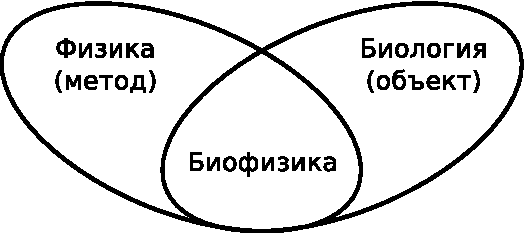
\includegraphics[width=5cm]{figures/fig_1_1.pdf}
 \caption{Вклад физики и биологии в биофизику.}
\end{figure}

Физика --- наука о природе, изучающая простейшие и вместе с тем наиболее общие свойства материального мира. Биофизика использует методы физики.

Биология --- совокупность наук о живой природе. Биология устанавливает общие и частные закономерности, присущие жизни во всех ее проявлениях и свойствах. Биология определяет объект исследования для биофизики.

PIT. Физика потерпела фиаско в биологии поскольку использовались слишком простые модели.


{\bf Теоретический опыт физики}

Одним из заблуждений наивного физика является представление о том, что гипотезы и теории физики представляют собой лишь сконденсированный опыт, индуктивный синтез экспериментальных данных \cite{Bunge1975}.

\begin{quote}
<<Даже наиболее „практичные“ из формул теоретической физики --- формулы физики твердого тела --- содержат более или менее изощренные теоретические понятия, далекие от непосредственного опыта. Более того, гипотезы и теории скорее выделяют опыт, нежели суммируют его, ибо они наводят на мысль о новых наблюдениях и экспериментах. Однако не это наиболее важно в функциях гипотез и теорий. Мы ценим их в первую очередь потому, что они позволяют нам более или менее схематично дать набросок реальности и приближенно и постепенно объяснять последнюю>> \cite{Bunge1975}.
\end{quote}



\newpage
%%%%%%%%%%%%%%%%%%%%%%%%%%%%%%%%%%%%%%%%%%%%%%%%%%%%%%%%%%%%%%%%%%%%%%%%%%%%%%%%%%%%%%%%
\section{Моделирование в биофизике}
{\it Понятие о моделях в методологии естественных наук. Теоретические и экспериментальные модели. Особенности биофизических моделей.}
% Блюменфельд Л.А. Информация, термодинамика и конструкция биологических систем // Соросовский образовательный журнал. 1996. № 7. P. 88–92.

\subsection{Понятие о моделях в методологии естественных наук}

% лекция 23.01.2003
Раз биофизика связана с изучением упрощенных сущностных конструкций, то без моделирования никуда.

% лекция 23.01.2013
Очень важно, что не указано, что является моделью, а что оригиналом --- так как их возможно поменять местами.


\subsection{Теоретические и экспериментальные модели}

Для решения ряда фундаментальных проблем биологии требуется высокий уровень обобщения, которого трудно достичь при изучении реальных биологических систем, поскольку исследованию общих свойств биологических систем препятствуют два фактора:
\begin{itemize}
\item высокая сложность реальных биологических объектов, приводящая к невозможности учета огромного количества взаимодействий, которые определяют функцию и свойства объекта;
\item единственность эволюционных исходов, которая не позволяет использовать один из самых эффективных инструментов исследования --- только один вариант живого, реализовавшийся на Земле).
В создавшейся ситуации одним из выходов, видимым в настоящее время, является обращение к эвристическим или, по-другому, феноменологическим моделям.
\end{itemize}

Необходимость перехода к искусственным модельным объектам обосновал фон Нейман: <<Поскольку у нас нет достаточно ясного представления о том, как функционируют живые организмы, то обращение к органике большой пользы нам не принесет. Мы займемся поэтому автоматами, которые мы в совершенстве знаем, ибо мы их сделали. Опишем автоматы, способные воспроизводить себя>>.

Обобщая специфику использования эвристических моделей, можно сформулировать понятие {\bf эвристического модельного объекта (ЭМО)}. Под моделью подразумевается следующее: {\bf <<Если между двумя объектами может быть установлено сходство хотя бы в каком-либо одном определенном смысле, то между этими объектами существуют отношения оригинала и модели>>}.



ЭМО --- это сконструированный формальный объект, соответствующий в определенном смысле широкому классу реальных объектов. ЭМО предназначен не для имитации поведения некоторой конкретной системы, а для выяснения общих зависимостей поведения системы от ее структуры и свойств ее компонентов.

ЭМО является моделью, но он отличается от традиционной модели по способу работы с ним. ЭМО выступает как полноправный (пусть и абстрактный) объект, отличающийся от реальных только тем, что он доступнее для экспериментирования. Абстрактный модельный объект <<прозрачен>>, про его структуру известно все и это позволяет сконцентрировать усилия непосредственно на выявлении общих закономерностей, а не на поиске кажущихся важными, а по сути бесконечных, деталей структуры. Применимость результатов, полученных с помощью ЭМО, зависит от степени общности задаваемых модельному объекту вопросов.

Работа с ЭМО принципиально отличается от традиционных способов моделирования. При создании математических моделей производится подборка параметров, для того чтобы они лучше описывали свойства моделируемых систем. В ЭМО же подборки параметров не происходит, поскольку нет реальной системы-оригинала. В процессе выявления закономерностей и свойств, демонстрируемых ЭМО, производится поиск закономерностей и свойств-аналогов в реальных системах. Это позволяет оценить адекватность положенных в основу построения ЭМО общих предположений. При обнаружении таких свойств-аналогов можно говорить об адекватности и общности, положенных в основу ЭМО предположений. Тогда те свойства ЭМО, которые не имеют известных аналогов в реальных системах или еще не попадали в фокус внимания исследователей, могут лечь в основу новых общих утверждений или гипотез о свойствах реальных систем.


\subsection{Особенности биофизических моделей}

% лекция 23.01.2013
Методология биофизики --- в основе лежат теоретические конструкты.

В биологии тоже есть такие теоретические конструкты, например --- Мендель предложил законы наследования.

Сцепленные гены, кроссинговер и т.д. открыли благодаря тому, что удалось с помощью конструкта упорядочить экспериментальные закономерности и увидеть отклонения.

Теоретические модели не значит, что они математические.

Биос --- возможно рассматривать как модель биосферы, например.

Экспериментальные модели --- модели самолетов в аэродинамической трубе.

Модельный объект --- горох, дрозофила. Полученные на них результаты --- распространяются на других растений и насекомых.


{\bf Сложность в биофизике} --- моделируемые системы невероятно сложные. Нужно ухитриться вычленить наиболее существенные свойства для исследуемых параметров. Хороших моделей биологических систем --- достаточно мало: транспорт через мембраны, популяции, сосуды у растений, микротрубочки, Ходжкина-Хаксли.

Модели всей клетки. Теория категорий. Категории --- самый верх абстракции. Но выводы в такой модели --- тривиальный. Связано с тем, что не выработана антология. См. "Эвристические модели в биофизике".

Нет модели в которая бы цепляла самую суть живого :(






\newpage
%%%%%%%%%%%%%%%%%%%%%%%%%%%%%%%%%%%%%%%%%%%%%%%%%%%%%%%%%%%%%%%%%%%%%%%%%%%%%%%%%%%%%%%%
\section{Математический аппарат моделирования в биофизике}
{\it Примеры описания биологических процессов с помощью: обыкновенных дифференциальных уравнений; уравнений в частных производных; разностных уравнений; клеточных автоматов; формул теории вероятности.}

\subsection{Описания биологических процессов с помощью обыкновенных дифференциальных уравнений}

Для описания кинетического поведения биологических систем используют дифференциальные уравнения вида:
\begin{equation}
	\label{general}
	\frac{dx_i}{dt} = F_i(x_1, x_2, \dots, x_n), \qquad (i = 1, 2, \dots, n)
\end{equation}
где $F_i (x_1, x_2, \dots, x_n)$ --- нелинейные функции динамических переменных $x_i$.

Как правило, они состоят из нескольких слагаемых. Положительные члены описывают прибыль компонента $x_i$, отрицательные --- убыль. Для построения системы достаточно знать скорости притока и оттока каждого компонента и их зависимость от переменных.

В разных биологических системах в качестве переменных могут выступать различные измеряемые величины: в биохимии --- это концентрации промежуточных веществ, в микробиологии --- число микроорганизмов или их суммарная биомасса, в экологии --- численность вида, в биофизике мембранных процессов --- мембранные потенциалы и т.д. Параметрами могут служить температура, влажность, рН, электрическая проводимость мембраны.

Процессы, происходящие в биологических системах, как правило, существенно нелинейны, соответственно нелинейны и модели этих процессов. В модели таких реакций правые части уравнений содержат нелинейные члены, что может создать математические трудности в их решении.

На многие существенные вопросы, касающиеся качественного характера поведения системы, отвечают методы качественной теории дифференциальных уравнений. Эти методы позволяют выявить важные общие свойства модели, не прибегая к нахождению в явном виде неизвестных функций $x_1(t), x_2(t), ..., x_n(t)$.

Различные функциональные процессы в биологических системах и их подсистемах сильно отличаются друг от друга по характерным временам протекающих в них процессов. Так, в целостной биологической системе одновременно протекают быстрые процессы ферментативного катализа (характерное время оборота фермента $\tau = 10^{-1}$--$10^{-5}$c), физиологические процессы (характерное время --- минуты) и процессы репродукции (от нескольких минут и более).

В ряде случаев в биологических системах осуществляется известный принцип узкого места (общая скорость превращения вещества во всей цепи реакции определяется наиболее медленной стадией). Именно наличие такой временной иерархии процессов позволяет существенно упростить исходную модель, по существу сведя задачу ее кинетического описания к изучению поведения наиболее медленной стадии. В этом смысле самое медленное звено --- управляющее, поскольку воздействие именно на него, а не на более быстрые стадии, может повлиять на скорость протекания всего процесса.

Рассмотрим {\bf пример понижения сложности модели с помощью временного масштабирования}. Пусть удалось представить систему (\ref{general}) в виде:
\begin{equation}
	\label{sepSystem}
 \left\lbrace 
	\begin{aligned}
		\varepsilon ^2 \frac{dx_i}{dt} &= F_i(x_1, x_2, ..., x_n), & i=1, ..., l,\\
		\varepsilon \frac{dx_j}{dt} &= F_j(x_1, x_2, ..., x_n), & j=l+1, ..., l+m,\\
		\frac{dx_k}{dt} &= F_k(x_1, x_2, ..., x_n), & k=l+m+1, ..., n.
	\end{aligned}
 \right.
\end{equation}

Тогда, если расположить по степеням малого параметра $\varepsilon$ при производной, коэффициенты $\varepsilon$ и $\varepsilon^2$ фактически определяют скорости изменения концентраций и система (\ref{sepSystem}) распадается на три независимых уравнения:

\begin{equation}
	\label{sepSystem2}
	\frac{dx_i}{dt} = \frac{1}{T_1} F_i, \qquad
	\frac{dx_j}{dt} = \frac{1}{T_2} F_j, \qquad
	\frac{dx_k}{dt} = \frac{1}{T_3} F_k, \qquad
\end{equation}
где $T_1 = \varepsilon^2$, $T_2 = \varepsilon$, $T_3 = 1$.

Если мы интересуемся поведением всех переменных, как на отрезках времени порядка $\varepsilon^2$, так и на временах порядка единицы, то необходимо исследовать всю систему. Если нет, то система значительно упрощается.



% лекция. Романовских 
Модели в частных производных...Одно время физическое, другое --- возраст клетки.

Пригожин --- диссипативные структуры.

Окрас --- по Алану Тьюрингу. Уравнения диффузии-реакции. Белоусова-Жаботинского.

{\bf ОДУ}
Популяции, и т.п.

{\bf Расностные уравнения}
Дискретные модели популяций 

{\bf Клеточные автоматы }
Жизнь и модель морфогенеза, и для исследования устойчивости, например, кучи. Критическая устойчивость кучи --- очень важная, поскольку аналогия с биосферой..???

Формула теории вероятности --- Марковские процессы. Освоение лабиринта.

Автоматы Цетлина.

Формулы теории вероятности. Связаны с Ур в частных производных.





\newpage
%%%%%%%%%%%%%%%%%%%%%%%%%%%%%%%%%%%%%%%%%%%%%%%%%%%%%%%%%%%%%%%%%%%%%%%%%%%%%%%%%%%%%%%%
\section{Управление и информация в биологических системах}
{\it Связь между понятиями <<управление>>, <<сигнал>> и <<информация>>. Необходимость введения понятий <<управление>> и <<информация>> для описания специфики биологических систем. Мышление человека, как предельный известный нам уровень обработки информации. Подход Р.~Пенроуза к проблеме сознания.}

\subsection{Связь между понятиями <<управление>>, <<сигнал>> и <<информация>>}

% лекция 23.01.2013
Волькенштейн говорил об этом в книге "Общая биофизика".



Сигнал информация, а информацию может обрабатывать только конструкция.


При обсуждении ключевых признаков живого мы пришли к заключению, что способность осуществлять выбор является универсальным признаком живого существа и не встречается в неживой природе естественного происхождения. Понятие <<выбор>> тесно связано с понятием <<управление>>.

Об этой тесной связи говорит и то, что известный А.А.~Ляпунов\footnote{Выдающийся советский математик, один из основоположников кибернетики. Не путать с его прадедушкой Александром Михайлович Ляпуновым, который жил веком ранее и разработал теорию устойчивости.} связывал специфику живого с наличием управления:
\begin{quote}
<<Для процессов жизнедеятельности характерно наличие специальных управляющих процессов. Последние отличаются тем, что передача небольших масс или порций энергии вызывает действия, состоящие в передаче гораздо больших энергий или масс. ...Управление можно объявить характеристическим свойством живого в широком смысле>>.
\end{quote}

Использование понятия <<управление>> невозможно без понятий <<цель управления>>, <<сигнал>>, <<датчик>>, <<рабочий орган>> и др. Эти понятия не относятся к понятиям физики. Но они не кажутся чужеродными в отношении биологических систем. Действительно, <<цель>>, <<сигнал>>, <<ответная реакция>>, <<рецептор>> (датчик), <<эффектор>> (рабочий орган) --- это слова из биологического словаря.

К сожалению, как это является обычным для начальных базовых понятий, нет общепринятых определений понятий управления и сигнала. Например, в технических отраслях знаний термин <<сигнал>> (signal, от латинского signum --- знак) очень часто используется в широком смысловом диапазоне, без соблюдения строгой терминологии. Фактически эти понятия являются неопределимыми, и мы можем получить о них представление, рассматривая работу системы управления в целом, и вводя, для определенности, рабочие (то есть для данного конкретного случая) определения.

Для определения сигнала можно обратиться к приведенной выше цитате. {\bf Сигналом называется передача небольших масс или порций энергии, которые вызывают действия, состоящие в передаче гораздо больших энергий или масс.} Тогда многие процессы в живом организме находят свое естественное описание в терминах сигнала и управления. Например, фотон, попавший в светочувствительный элемент глаза, запускает целый каскад реакций, который завершается возникновением нервного импульса, который, в конечном счете, после его обработки в мозгу может завершиться реагированием всего организма. Очевидно, что энергия фотона и энергетические затраты организма, связанные с его реакцией на сигнал не сопоставимы. Другим примером может служить аллостерическая регуляция активности какого-либо фермента, когда изменения в количествах молекул регулятора и продукта ферментативной реакции также не сопоставимы.

Появление определенного сигнала, вызывает конкретную реакцию биологической системы в определенных условиях, что означает осуществление выбора. Например, бактерия, попав в новую среду изначально <<не знает>> ее состава, а значит <<не знает>> какой набор транспортных ферментов необходим для роста. И только получив от рецепторов соответствующие сигналы, бактерия <<решает>> что ей нужно синтезировать для роста на данной среде. То есть бактерия осуществляет выбор, и поступление определенных сигналов с рецепторов уменьшило исходную неопределенность этого выбора. В данной ситуации напрашивается употребление еще одного широко распространенного термина <<информация>>. Можно сказать, что бактерия получила информацию о состоянии среды и эта информация помогла ей осуществить правильный, выбор.

{\bf Что же такое информация?}

Этимология термина <<информация>> восходит к латинскому глаголу informare --- придавать форму разуму (интеллекту), формировать идею (представление о чем-либо) --- обучать, инструктировать, дисциплинировать, тренировать. Информирование --- это процесс, в результате которого разум приобретает форму. В этом смысле <<информирование>> сходно со славянским <<образованием>>, в основе которого --- образ, <<обрезать>>, то есть отрезать лишнее. 
Исторически так сложилось, что измерять количество информации стали раньше, чем дали определение самой информации. 

Мера количества информации была введена К.Э.~Шенноном в 1948~г \cite{Shannon1948}. Количество информации в сообщении, содержащем $N$ символов $I_N$, по Шеннону равно:
\begin{equation}
	\label{infoShen}
	I_N = -N \sum_{i=1}^M p_i \log_2 p_i,
\end{equation}
где $M$ --- число букв в алфавите,\\
$p_i$ --- частота встречаемости $i$-ой буквы в алфавите.

Двоичные логарифмы выбраны для удобства. При однократном бросании монеты $M = 2$, $N = 1$, и $p = 1 / 2$. При этом получаем минимальное количество информации ($I = 1$), которое называется <<бит>>.

В общем случае, когда делается выбор одного варианта из $n$ возможных (реализующихся с априорной вероятностью $p_i, i = 1, 2, ..., n$) количество информации выражается формулой:
\begin{equation}
	\label{infoShen2}
	I_N = -N \sum_{i=1}^n p_i \log_2 p_i, \qquad \text{где} \quad i = 1, 2, ..., n.
\end{equation}

Если все варианты равновероятны, т.е. $p_i = 1 / n$, то: $I = \log_2 n$.

Выражения (\ref{infoShen}) и (\ref{infoShen2}) описывают количество полученной, переданной, обработанной информации. Но информация иметь еще одну важную характеристику --- ценность. Соотношение количества информации и ее ценности представляется важным для дальнейшего рассмотрения. Если любое сочетание букв в тексте является ценным, то количество ценной информации совпадает с ее полным количеством, но не может превышать ее. Это значит, что любая передача сигналов может содержать какое-то количество ценной (или осмысленной) информации, но может содержать и меньшее и не содержать вовсе. В этой связи количество информации в (\ref{infoHarkevich}) можно назвать информационной тарой. Это понятие играет существенную роль при рецепции информации и/или обработке ее (в частности при перекодировке). Приведем пример.

Имеется текст на русском языке, содержащий $N_r$ букв кириллицы (алфавит содержит 32 буквы). Перевод его на английский язык содержит $N_e$ букв латинского алфавита (26 букв). Русский текст --- результат выбора определенного варианта из $n_r = 32^{N_r}$ возможных. Английский перевод --- выбор определенного расположения латинских букв, который предопределен русским текстом (рецепция информации). Число вариантов в английском тексте порядка $26^{N_e}$. Количество ценной информации одинаково (если смысл не искажен), а количество информации различно. 

Процессы генерации, рецепции и обработки ценной информации, сопровождаются <<переливанием>> информации из одной тары в другую. При этом, как правило, количество информации уменьшается, но количество ценной информации сохраняется. Пример, процесс трансляции генетической информации. Иногда <<информационные тары>> столь различны, что можно говорить об информациях разного типа. Этот термин применяется к информациям, имеющим одинаковый смысл и ценность, но сильно различающимся количественно, т.е. помещенными в разные тары. 
Но поскольку мы вышли к понятию информации через управление и осуществление системой выбора, то в контекст нашего рассмотрения лучше вписывается следующее рабочее определение: <<{\bf информация есть мера уменьшения неопределенности выбора}>>.

Это определение практически совпадает с мерой ценности информации, предложенной А.А.~Харкевичем:
\begin{equation}
	\label{infoHarkevich}
	V = \log_2 \frac{P}{p},
\end{equation}
где $p$ --- вероятность достижения цели {\bf до} получения информации,\\
$P$ --- вероятность достижения цели {\bf после} получения информации.

Априорная вероятность зависит от информационной тары или, что то же, полного количества информации $I$ в (\ref{infoShen2}): $p = 2 - I$. Так, если до получения информации все варианты равновероятны, то $p = 1/n$ (где $n$ --- число вариантов).

Апостериорная вероятность $P$ может быть как больше, так и меньше $p$. В последнем случае ценность отрицательна и такая информация называется дезинформацией. Примером последней является червеобразный отросток над губой глубоководного курильщика, который привлекает жертв. Вид этого отростка несет отрицательную информацию с точки зрения целей жертвы. Таким образом, вероятность $P$ находится в пределах $0 < P < 1$, и соответственно, $ -\infty < V < V_{max}$.

Мера ценности информации, предложенная В.И.~Корогодиным:
\begin{equation}
\label{infoKorogod}
V = \frac{P - p}{1 - p}
\end{equation}
где обозначения совпадают с (\ref{infoHarkevich}).

Эта мера обладает теми же свойствами, что и (\ref{infoHarkevich}), но изменяется от $0$ до $1$, что иногда удобнее при сравнении ценностей информации в разных процессах ее возникновения, передачи и обработки.

Согласно (\ref{infoHarkevich}) ценность информации зависит от величины $p$ --- вероятности достижения цели до получения информации, т.е. от того, какой предварительной (априорной) информацией уже располагает система, принимающая решение. Предварительная осведомленность называется тезаурусом. Если таковая отсутствует, то априорная вероятность во всех вариантах одинакова и равна $p = 1/n$ (где $n$ --- число вариантов).Если при этом после получения информации цель достигается наверняка ($P = 1$), то ценность этой информации максимальна и равна $V = V_{max} = \log_2 n$, то есть совпадает с максимальным количеством информации в данном множестве (в данной таре). Это совпадение не случайно, именно для этого была выбрана форма (\ref{infoHarkevich}), при этом ценность информации можно понимать как количество ценной информации. Ценность информации субъективна.

Существует информация, которая на первый взгляд, ни для кого и никогда не может стать ценной. Пример: в тексте наборщик, переставил буквы так, что текст потерял всякий смысл. Количество информации сохранилось, но ценность его для кого бы то ни было, стала равна нулю. Так появляется понятие <<осмысленность>>. В отличие от <<ценности>> это понятие претендует на объективность, что основано на следующем положении: в информационной таре, куда вмещена данная информация, можно выделить определенное количество информации, которая никогда ни для кого ни для какой цели не понадобится. Тогда эту информацию называют лишенной смысла. Объективность критерия основана на утверждениях: <<ни для кого, никогда, ни для какой цели>>. Это определение сильное, абсолютное, и как таковое, конечно не применимое к реальности. Так в приведенном примере можно сказать, что абракадабра, которую сотворил наборщик содержит ценную информацию для психиатра, цель которого --- поставить наборщику диагноз. Поэтому утверждение <<ни для кого>> следует понимать: ни для кого, кого интересует смысл текста и ничего более.

Вопросы ценности и осмысленности информации особенно важны в отношении биологических систем, поскольку возникновение живого и его эволюция представляют собой возникновение ценной информации и ее эволюцию. Ценность информации эволюционирует: неценная информация становится ценной, бессмысленная --- осмысленной и наоборот.



\subsection{Подход Р.~Пенроуза к проблеме сознания}

Проблема взаимодействия материального и идеального...

Оказывается никак, поскольку материальное определяет мысли...

Микротрубочки. Принцип суперпозиции... двух конформаций $\alpha$ и $\beta$. Сознание связано с квантовой нелокальностью с парадоксом Эйнштейна-Подольского. Микротрубочки как изолятор от квантового шума...





\newpage
%%%%%%%%%%%%%%%%%%%%%%%%%%%%%%%%%%%%%%%%%%%%%%%%%%%%%%%%%%%%%%%%%%%%%%%%%%%%%%%%%%%%%%%%
\section{Редукционизм и холизм в исследовании биологических систем}
{\it Функциональное и структурное описания живых систем. Живые организмы как $(M, R)$-системы по Р.~Розену. Понятие замкнутости по эффективной причине.}

\subsection{Функциональное и структурное описания живых систем}

Холизм (англ. {\it whole} --- весь) --- рассмотрение биологической системы как целого.

Понимание моделирования в биологии начинается с понимания взаимодействия физики и биологии. Биологические организмы состоят из атомов и молекул, значит, они --- физические системы.

Фундаментальный принцип редукционизма в биологии состоит в том, что у нас нет реального понимания биологической активности, пока это понимание не выражено в терминах взаимодействия между физическими частицами, из которых состоит организм.

С точки зрения редукционизма, не существует полезных различений между органическим и неорганическим; между биологией и физикой. Инструменты, для наблюдения биологических систем, и теоретические конструкты, для их описания, взяты из небиологических дисциплин.

{\bf Системы и их описание}

{\bf Внутреннее описание систем.} Описать, на что похожа система в данный момент времени, означает определить {\it состояние} системы. Множество всех возможных состояний системы, позволяющее оценить ее в любой момент времени называется {\it пространством состояний системы}. В физике эти состояния определяются через измерение, численно выражаемых показателей, называемых {\it существенными переменными (СП)} или {\it переменными состояния} и обладающие следующим свойством: если 2 состояния различаются при любых способах наблюдения, то также различаются по СП, и наоборот, если 2 состояния идентичны по СП, то они не различаются по другим наблюдаемым показателям.

{\bf Внешнее описание.} Вместо переменных состояния имеется семейство возмущений или воздействий, которые мы можем оказывать на систему, называемых {\it входами системы} и набор наблюдаемых величин, которые используются для обозначения эффекта воздействия входов на систему, называемых {\it выходами или откликом системы}. В соответствии с этим подходом задача заключается в прогнозе отклика системы на произвольное входное воздействие.

Одна из целей науки есть совмещение этих 2-х видов системного описания. Внешнее описание --- это {\it функциональное описание}; оно говорит нам, ЧТО система делает, но не то, КАК она это делает. Внутреннее описание --- это {\it структурное описание}; оно говорит нам, КАК система делает то, ЧТО она делает, но практически не содержит функциональное содержание. Проблема заключается в эффективном переходе между 2-мя описаниями: {\it проблема структуры-функции}!
Теоретическая физика доминирует благодаря внутреннему описанию, поскольку природные системы, с которыми физик имеет дело, в общем случае достаточно просты и понятие <<функция>> к ним не применимо. Внешнее описание становится важным, когда мы обсуждаем искусственные системы, особенно управление и регуляцию машин, которые мы для себя сделали.
Биологические системы построены на существенно отличных (и по большей части неизвестных) принципах по сравнению с искусственными системами. При этом наше описание организмов есть смесь внутренних и внешних характеристик. Многие типы биологической активности фактически определены и наблюдались только функционально в терминах {\it внешнего описания}. С другой стороны, в биологии много экспериментальных подходов взятых из физики для получения огромного количества разнообразной структурной информации.

Однако переменные внутреннего состояния, которые относительно легко измеряемы, не связаны простым отношением с функциональной активностью биологических систем и наоборот, внутреннее описание, подходящее к функциональному поведению биологических систем, не связано простым отношением со структурными наблюдаемыми величинами, измеряемыми физическими методами.

{\bf Подходы к исследованию сложных систем}

Гипотеза редукционизма говорит, что базовые свойства биологических систем могут быть эффективно поняты в терминах внутреннего физического описания. Возникает вопрос, как может физик подходить к системе, которая слишком сложна, чтобы допускать исследование в целом? Обычным подходом является абстрагирование или упрощение системы, обычно достигаемое путем разделения исходной системы на подсистемы. И так до тех пор, пока полученные подсистемы не будут допускать исследование как целое.

Неявно здесь допускается две ключевые гипотезы теоретико-системного характера:

\begin{enumerate}
\item Любая физико-химическая система, даже сложная, может быть разложена на спектр подсистем, таких, что каждая из подсистем в отдельности может быть полностью понята;
\item Любое свойство исходной системы может быть реконструировано из соответствующих свойств выделенных подсистем.
\end{enumerate}

Последняя гипотеза очевидно неверна, о чем говорит ряд примеров из физики и биологии.

Утверждается, что методика разделения системы на подсистемы, пришедшая в биологию из физики в общем случае не совместима с динамикой биологических систем. 
Она будет отличной от привычной методики для аналитической биологии.

{\bf Системные аналоги}

Существует промежуточный между внутренним и внешним описанием подход к исследованию биологических систем, позволяющий продвинуться дальше, чем при использовании только внешнего описания. Имеется в виду использование систем-аналогов или модельных систем, которые используются при исследовании сложных систем, включая биологические. Модели ферментов, мембран, искусственные нейросети и т.п. Подход основан на том, что одни и те же динамические или функциональные свойства могут принадлежать огромному классу систем разнообразной природы.

Две системы, которые физически различны, но динамически эквивалентны, называются аналогами друг друга. Моделирование с помощью системных аналогов полностью отличается от метода разложения системы на подсистемы! Системная аналогия показывает, что динамические или функциональные свойства могут быть исследованы независимо от специфики физико-химической структуры, важной при редукционизме.

Пример подхода в физике --- оптико-механическая аналогия и вариационные принципы.

\textbf{{\it{\bf Утверждение}}}: любое функциональное или динамическое свойство данной системы может быть исследовано одинаково хорошо на любом из системных аналогов или даже целиком абстрактно. Такое абстрактное функциональное свойство, проявляемое каждым из системных аналогов, которые реализуют абстрактную систему назовем {\bf динамической метафорой}.

На этом пути можно начать развивать то, что может быть названо <<функциональным разделением (фракционированием)>>, которое дает возможность видеть следствия простейших динамических свойств некоторой метафоры, а также необходимость более специфических динамических или структурных предположений. Примеры метафор: открытые системы, переключающиеся системы, пороговые элементы, эквифинальность в развитии и регенерации.

Проблема в том, что типичный биолог требует привязки наблюдаемых функций к конкретной биологической структуре, которую он исследует. Можно предположить, что динамические метафоры, дополненные условиями (в частности, ограничениями, возникающими из рассмотрения оптимальной конструкции) дадут возможность выбирать отдельную систему из огромного класса систем-аналогов (именно ту, которая удовлетворяет дополнительным ограничениям оптимальности) и относительно этой выбранной системы можно сделать гораздо больше специфических заключений о ее структуре.


\subsection{Живые организмы как ($M$, $R$)-системы по Р.~Розену}

(M,R)-система (от англ. Metabolism, Repair --- метаболизм и ремонт) --- математическая модель клеточного метаболизма, сформулированная Робертом Розеном в 1957 году[1][2] с использованием аппарата теории категорий.

Метаболизм и ремонт заданы в качестве отображений.

Размножение появляется само собой, неявно.

Предсказывающее поведение задается граничными условиями.



{\bf Метафора метаболизма Р.~Розена \cite{Rozen1969}}

{\bf Введение в терминологию}. Аристотель развил множество причинных ответов на вопрос <<почему>>, которое открывает совершенно новую сферу (область) описания в системах. Эти причины могут быть проиллюстрированы как ответы на вопрос о причинах существования дома. Ответами на вопрос <<Почему этот дом стоит здесь?>> являются:
\begin{itemize}
\item Материальная причина: кирпичи, дерево, метал, стекло \dots
\item Деятельная (эффективная) причина: те, кто собрал из материалов дом, --- строители, производитель \dots
\item Формальная причина: планы и чертежи, что позволили собрать материалы в форму;
\item Финальная причина: причина постройки дома: деньги заплатили, быть местом для жилья.
\end{itemize}

{\bf Замкнутость по эффективной причине}

Материальные причины --- сплошные стрелки, пунктирные --- действующие причины.

\begin{figure}[ht]
	\center
	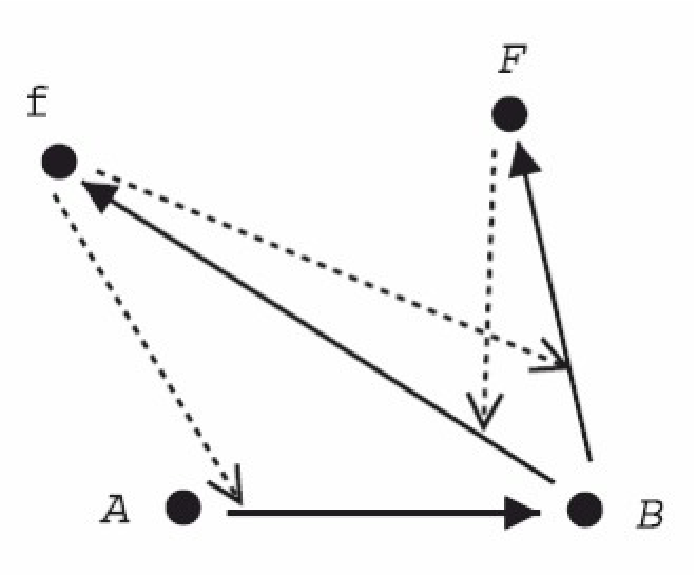
\includegraphics[width=6cm]{figures/Rozen2.pdf}
	\caption{Механизм обеспечения замкнутости метаболизма по действующей причине}
\label{figCurves}
\end{figure}

{\bf Еще один вариант обеспечения замкнутости метаболизма по действующей причине}


{\bf Наивный взгляд на метаболизм}

В этом простом примере единственная метаболическая функция организма заключается в производстве метаболита $ST$ и предшественников $S$ и $T$, присутствующих в окружающей среде. Она требует катализатора, молекулы $M$, но иллюстрация не отражает тот факт, что $M$ имеет неустранимую тенденцию к распаду, то есть система может существовать только ограниченное время.

{\bf Метаболический пример ($M$, $R$)-системы}

\begin{figure}[ht]\center
 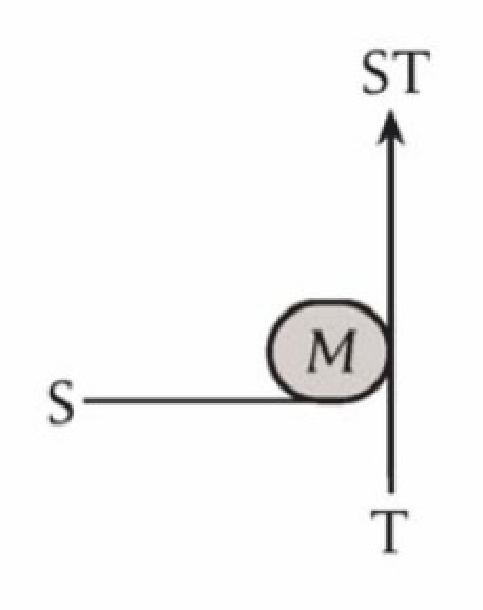
\includegraphics[width=3cm]{figures/Rozen3.pdf}
\end{figure}

\begin{itemize}
\item [(a)] исходная модель расширена с учетом распада катализатора $M$, который сейчас восстанавливается благодаря активности второго катализатора $R$, действующего на третий внешний субстрат $U$. Сам $R$ восстанавливается в результате вторичной активности $M$, действующего на $U$ как альтернативный к $S$ субстрат. Восстановительный модуль показан серым;



\item[(b)] катализаторы представлены структурами $STU$ и $SU$, и каждый каталитический процесс представлен как цикл из трех реакций, например $STU\to STUS\to STUST$, чтобы сделать химическую структуру катализа явной.
\end{itemize}

\begin{figure}[ht] \center
	\begin{multicols}{2}
	\hfill
	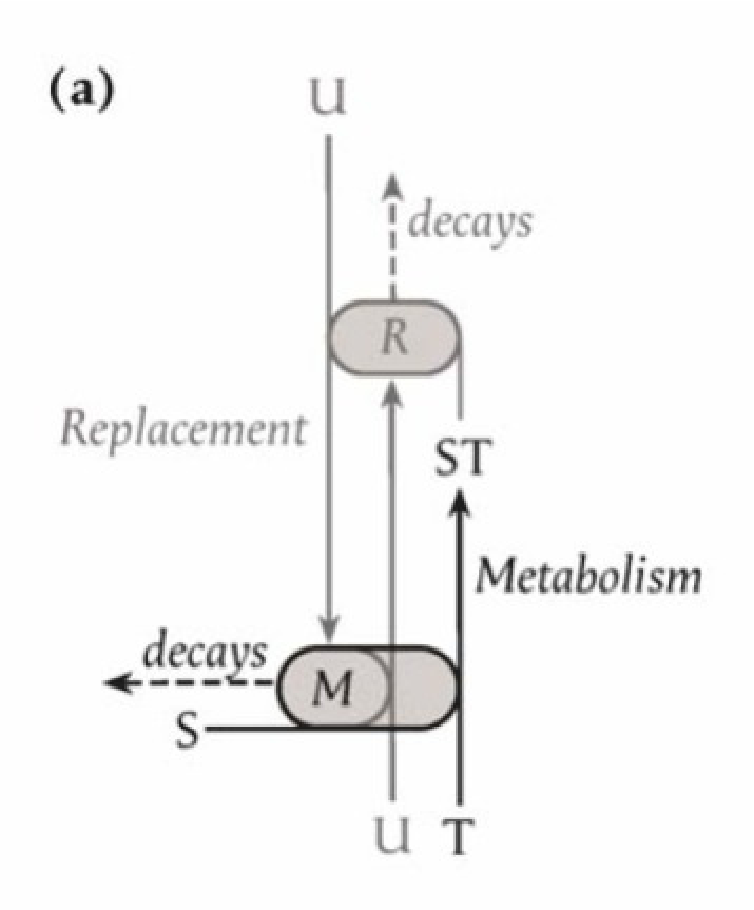
\includegraphics[width=4cm]{figures/Rozen4.pdf}
	\hfill
	\caption{\small Исходная модель, расширенная с учетом распада катализатора $M$}
	\label{figLeft}
	\hfill
	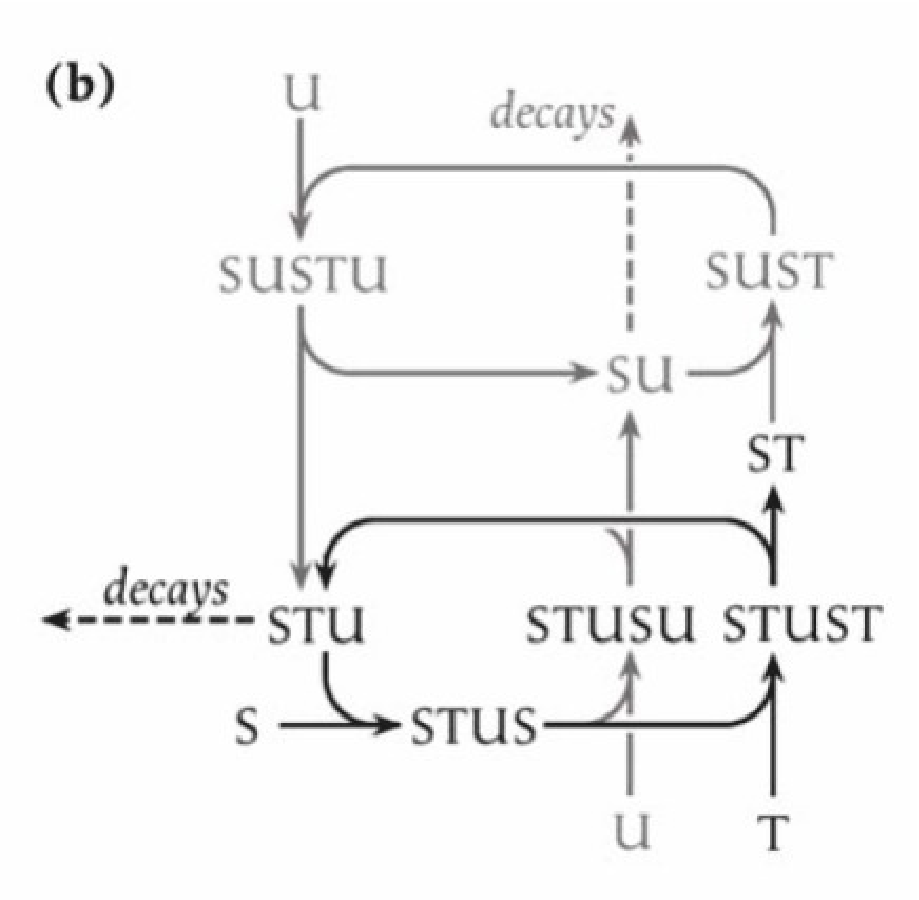
\includegraphics[width=4cm]{figures/Rozen5.pdf}
	\hfill
	\caption{\small Катализаторы представлены структурами $STU$ и $SU$}
	\label{figRight}
 \end{multicols}
\end{figure}



Ковач (2006) отметил, что <<биологи должны помнить, что жизнь написана на языке химии>>. Верно, но они должны также помнить оригинальную версию Галилея, что природа написана на языке математики, поскольку полностью удовлетворительная теория жизни будет требовать не только всех биологических деталей, которые подчиняются законам химии и термодинамики, но также математического формализма того сорта, который Розен пытался развивать.


\subsection{Понятие замкнутости по эффективной причине}




\newpage
%%%%%%%%%%%%%%%%%%%%%%%%%%%%%%%%%%%%%%%%%%%%%%%%%%%%%%%%%%%%%%%%%%%%%%%%%%%%%%%%%%%%%%%%
\section{Экстремальные принципы в биологии}
{\it Физическая каузальность и биологический финализм. Принципы максимальной простоты, оптимальной конструкции, адекватной конструкции. Частные принципы оптимальности.}

\subsection{Физическая каузальность и биологический финализм}

% Волькенштейн М.В. Общая биофизика. Москва: Наука, 1988. P. 592. стр. 15

Биологическая эволюция определяется преимущественным выживанием популяций, более приспособленных к условиям среды. Соответственно строение организма характеризуется такой приспособленностью и адаптацией к определенной экологической нише. Поэтому в биологии естественным образом возникает финалистическая трактовка изучаемых явлений. Развитие зиготы во взрослый организм можно описывать, пользуясь понятием цели: целью развития является создание приспособленного организма. Уже на ранних стадиях эмбриогенеза определенные группы клеток предназначены для развития в определенный орган, и этим задается их функциональность на всех уровнях, вплоть до молекулярного \cite{Volkenshtejn1988}.

Организм подобен машине, построенной по плану для достижения определенных целей. Более того, это машина высшего уровня сложности, способная целесообразно реагировать на заранее не запланированные события. Пример --- производство организмом высшего животного антител в ответ на практически любые антигены, в том числе и искусственные, с которыми никогда не приходится встречаться в природе. Финалистическое описание непосредственно следует из историчности живых организмов. Оно не свойственно обычной физике и химии. Очевидна бессодержательность такого, например, утверждения: <<Ионы натрия и хлора взаимодействуют друг с другом для того, чтобы построить кубический кристалл>>. Напротив, утверждение <<...так как ионы $Na^+$ и $Cl^-$ имеют единичные заряды и такие-то радиусы, ионный кристалл $NaCl$ должен быть кубическим>> имеет ясный смысл \cite{Volkenshtejn1988}.

Биологи часто задают вопрос <<для чего?>>, физики спрашивают <<почему?>>. Очевидно, что истинный научный смысл имеет именно второй вопрос. Физика и естествознание в целом каузальны --- наука ищет причины (causa) явлений. В действительности нет противоречия между финализмом и каузальностью, и указанное различие между физикой и биологией является внешним. Финализм возникает в физике всякий раз, когда мы встречаемся с проблемами устойчивости, с вариационными принципами. Мы имеем в виду устойчивость в строгом математическом смысле, по Ляпунову (см. гл. 15). Устойчивое состояние динамической системы сохраняется при малых возмущениях --- система, будучи отклонена от этого состояния, в него возвращается. Финалистическая формулировка: система стремится сохранить свое состояние. Напротив, неустойчивое состояние необратимо изменяется при малом возмущении --- система стремится перейти в другое состояние. Пример --- состояния равновесия физического маятника, устойчивое и неустойчивое \cite{Volkenshtejn1988}.

Вариационный принцип всегда финалистичен. Так, согласно принципу наименьшего действия Гамильтона, вариация действия равна нулю, действие минимально. <<Цель механической системы состоит в ее наименьшем действии>>. Но, как показывает классическая механика, принцип Гамильтона эквивалентен уравнениям движения Лагранжа, в свою очередь следующих из второго закона Ньютона. Этот закон каузален, он описывает ускоренное движение как результат действия сил. Другие примеры финалистически формулируемых законов физики: принцип Ферма в оптике, принцип Ле Шателье в термодинамике, правило Ленца в электродинамике. Вариационный финализм сводится к каузальности. Число таких примеров неограниченно \cite{Volkenshtejn1988}.


\subsection{Принцип максимальной простоты}

Одни и те же функции при одинаковой их интенсивности, вообще говоря, могут выполняться несколькими различными структурами. В 1943 году был предположительно сформулирован принцип, согласно которому та конкретная структура или конструкция, которую мы действительно находим в природе, является {\it простейшей} из возможных структур или конструкций, способных выполнять данную функцию или группу функций.

Применение этого принципа состоит в рассмотрении различных механизмов (то есть моделей), способных выполнять заданную функцию. Из этих моделей выбирается самая простая. Затем к разным моделям применяется \textbf{принцип максимальной простоты}. Как всякий общий принцип он должен быть применим к любой данной ситуации. Однако нет <<единицы>> измерения простоты. И нечто простое, с точки зрения устройства, может быть сложным, с точки зрения формирования.

% лекция 23.01.2013
Рашевский --- принцип оптимальной простоты, какие его недостатки, почему он перешел к принципу оптимальной конструкции.


\subsection{Принцип оптимальной конструкции}

В 1954 году предложен принцип оптимальной конструкции, согласно которому органическая структура, необходимая для выполнения данной функции, должна быть оптимальна в отношении нужного количества материала и необходимых затрат энергии. 

Основная гипотеза заключается в том, что организмы, обладающие биологической структурой, оптимальной в отношении естественного отбора, оптимальны также и в том смысле, что они минимизируют некоторую оценочную функцию (принцип оптимальной конструкции). Эта функция определяется исходя из основных характеристик окружающей среды.

% лекция 23.01.2013
Рашевский и от него отказался, так как этот принцип неоптимальный. И пришел в итоге к принципу адекватной конструкции.

\subsection{Принцип адекватной конструкции}

Если задан некоторый набор функций организма или отдельного органа, то чтобы найти форму или структуру этого органа, биофизик должен идти таким же путем, каким идет инженер, конструируя устройство или машину для выполнения заданной функции. Конструкция должна быть адекватна заданной функции при заданных изменяющихся условиях среды.

Сформулированный принцип допускает, очевидно, не единственное решение проблемы формы и структуры. В органическом мире мы действительно находим организмы и органы, которые выполняют в основном одинаковые функции, но различны по своей форме. Однако организмы, выполняющие разные функции всегда различны по своей структуре. Так же обстоит дело и в технике. 

Например: Толщина тела должна быть примерно пропорциональна его длине в степени $3/2$. 


\subsection{Частные принципы оптимальности}


Одно из приложений принципа оптимальной конструкции --- {\bf моделирование кровеносной системы}. Рассмотрена задача нахождения оптимального угла отклонения боковой ветви от основного ствола. Радиусы ствола и ответвления известны: $r_0$ и $r_1$. В качестве оценочной функции выбирается сопротивление кровеносной системы, которое согласно принципу оптимальности должно быть минимальным (АДС на Рис. \ref{sosudi1}) \cite{Fursova2003}.
	
\begin{figure}[ht] \center
	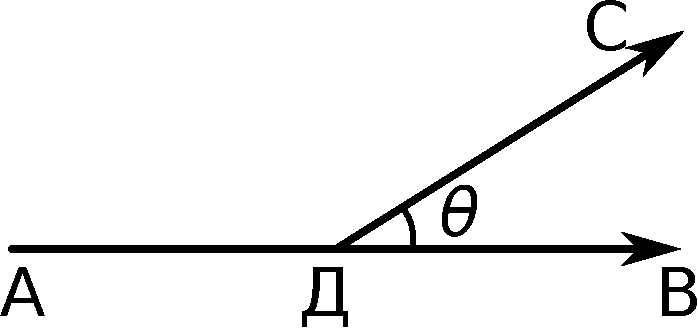
\includegraphics[width=4cm]{figures/Extrem1.pdf}
	\caption{Отхождение бокового сосуда \cite{Fursova2003}}
	\label{sosudi1}
\end{figure}
	
Полного сопротивления $RT$ участка АДС от угла ответвления $\theta$ зависит так:
\begin{equation}
R_T(\theta)=const+k\lambda_0 \left( \frac{\cosec\theta}{{r_1}^4} 
	- \frac{\ctg\theta}{{r_0}^4} \right),
\end{equation}
где $k$ --- коэффициент пропорциональности, зависящий от вязкости и плотности жидкости;\\
$\lambda_0$ --- длина отрезка $CB$.

Продифференцируем $R_T(\theta)$ по $\theta$ и приравняем результат нулю. Получим оптимальное значение $\theta$:
\begin{equation}
\theta_{min} = \arccos \left( \frac{{r_1}^4}{{r_0}^4} \right).
\end{equation} 

Следующим шагом является рассмотрение разветвления сосудов (рис. 2), где оценочной функцией здесь выступает мощность, рассеиваемая при движении жидкости.

\begin{figure}[ht] \center
	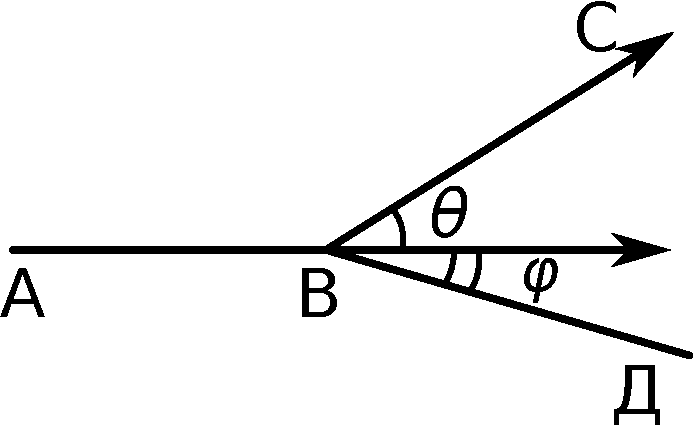
\includegraphics[width=4cm]{figures/Extrem2.pdf}
	\caption{Разветвление сосудов}
\end{figure}

\begin{equation}
	P_T = f^2 R_T + KV,
\end{equation}
где $f$ --- поток жидкости;\\
$K$ --- постоянный коэффициент пропорциональности;\\
$RT$ --- полное сопротивление;\\
$V$ --- объем изучаемого участка.

Полученные оптимальные значения углов разветвления сравнивали с реальными углами системы кровеносных сосудов кошки и получили хорошие совпадения. Оптимальный радиус аорты, обеспечивающий экономию материала и одновременно предотвращающий возникновение турбулентности, тоже соответствует реальности. То же относится к параметрам сердечного цикла, ударным объемом сердца, диапазон изменений кровяного давления между систолой и диастолой.

Развитие описанных методов позволяет найти оптимальный радиус отходящей ветви, радиус аорты, а также общее число капилляров, в предположении, что сосуды образуются в результате разветвления более крупного сосуда. Полученные результаты совпадают с эмпирическими данными.

{\bf Принцип минимума общего осмотического давления}. С.~Шустер и Р.~Гейнрих применяли метод условной экстремизации при изучении стационарного течения биохимических реакций. Они принимают, что общее осмотическое давление промежуточных продуктов в реакции можно записать в виде:
\begin{equation}
	\Omega = \sum_{i=1}^n g_i(x_i)x_i,
\end{equation}
где $x_i$ и $g_i$ обозначают, соответственно, концентрацию и коэффициент осмотического давления $i$-го промежуточного продукта реакции (зависимость $g_i$ только от $x_i$ является упрощающим предположением).

Естественно, что осмотическое давление в клетке не может превосходить некоторой критической величины. Поэтому авторы считают, что при стационарном течении реакции, при котором все $x_i$ не зависят от времени, $\Omega$ должно принимать минимальное значение при ограничениях:
\begin{equation}
\sum_{i=1}^n c_{ij} \ln x_j \le \ln\widehat{q}_j, \ j=1, \dots, r 
\end{equation}
где $\widehat{q}_j$ --- некоторые равновесные константы реакции,\\
$c_{ij}$ --- элементы стехиометрической матрицы реакционной системы.

Таким образом, при стационарном течении реакции, концентрации промежуточных продуктов, $i=1,\dots, n$, находятся как решения следующей задачи:
\begin{equation}
	\label{feMinPress}
 \left\lbrace 
	\begin{aligned}
		&\sum_{i=1}^n g_i(x_i)x_i\to min;\\
		&\sum_{i=1}^n c_{ij} \ln x_j \le \ln\widehat{q}_j, \ j=1, \dots, r. 
	\end{aligned}
 \right.
\end{equation}

{\bf Логистическое уравнения как экстремаль функционала действия.} Один из способов применения целевой функции состоит в формулировании общего утверждения относительно поведения системы. Хорошо известные экстремальные принципы относятся к этому случаю. В экологии предпринимались попытки использования этого подхода для получения уравнения роста популяции, точнее, рассматривалась обратная задача: записать действие, которое приведет к специальному уравнению роста.
	
В качестве функционала действия, который приведет к логистическому уравнению роста популяции численности $n$, было рассмотрено следующее выражение:

\begin{equation}
S=\int \left[ \frac{1}{2} \left( \frac{\overset{.}{n}}{n} \right)^2+ \frac{1}{2} r^2 \left( 1- \frac{n}{k} \right)^2 \right] \,dt
\end{equation}

Для упрощения вычисления была сделана замена переменных:
   
\begin{equation}
\label{feMinPress1}
 \left\lbrace 
	\begin{aligned}
		&S=\int \left[ \frac{1}{2} \overset{.}{x}^2 - V(x) \right] \,dt \text{, где \ } x=\ln \left( \frac{n}{k} \right);\\
		&V(x)=-\frac{1}{2}r^2(1-e^x). 
	\end{aligned}
 \right.
\end{equation}

Согласно вариационному принципу, уравнение эволюции $x(t)$ задается требованием $dS=0$ (экстремальность действия). После вычислений получим динамическое уравнение

\begin{equation}
	\overset{..}{x}^2=-r^2e^x(1-e^x).
\end{equation}

Чтобы сравнить этот результат с логистическим уравнением 
\begin{equation}
	\frac{dn}{dt}=rn\left( 1- \frac{n}{k} \right),
\end{equation}
его переписали в переменных $x=\ln \left( \frac{n}{k} \right) \Rightarrow \overset{.}{x}=r(1-e^x)$ и продифференцировали: 
\begin{equation}
	\overset{..}{x}^2=-r^2e^x(1-e^x).
\end{equation}

Полученное совпадение показывает, что любое решение логистического уравнения является решением динамического уравнения, выведенного из функционала действия. Однако не любое решение уравнения $\overset{..}{x}^2=-r^2e^x(1-e^x)$ является решением логистического уравнения. Для выявления взаимосвязи между данными уравнениями было проведено исследование полученного уравнения эволюции. После соответствующих преобразований и интегрирования было получено выражение
\begin{equation}
	\frac{1}{2} \left( \frac{\overset{.}{n}}{n} \right)^2 +
		\frac{1}{2} r^2 \left(1 - \frac{n}{k} \right)^2 = R, \ R=const
\end{equation}
 
Уравнение эволюции характеризуется константой $R$: при $R > 0$ популяция неограниченно растет, при $R < 0$ популяция достигает максимального значения, а затем уменьшается до 0. Значение $R = 0$ приводит к логистическому уравнению, тем самым, показывая, что логистический рост --- это особый случай равновесия между неограниченным ростом и затуханием:
\begin{equation}
S=\int \left[ \frac{1}{2} \left( \frac{\overset{.}{n}}{n} \right)^2+ \frac{1}{2} r^2 \left( 1- \frac{n}{k} \right)^2 \right] \,dt
\end{equation}
 
Рассмотрен также вопрос об интерпретации введенного таким образом <<биологического>> действия. 

Описание в терминах кинетической и потенциальной энергии неприемлемо, поскольку ведет к неизменности общей энергии системы (экологические системы обычно подразумеваются открытыми). 

По аналогии с физикой, где действие разделено на свободное движение и взаимодействие, предлагалось рассматривать введенное действие как сумму члена, описывающего популяцию, которая не подвержена помехам в росте, и члена $V(x)$, описывающего внешнее влияние среды на популяцию. Однако, подобная интерпретация хорошо описывает лишь случай $V(x) = 0$, когда применение вариационного принципа приводит к уравнению экспоненциального роста.




\chapter{Проблема жизни}

%%%%%%%%%%%%%%%%%%%%%%%%%%%%%%%%%%%%%%%%%%%%%%%%%%%%%%%%%%%%%%%%%%%%%%%%%%%%%%%%%%%%%%%%
\section{Атрибуты живого с эволюционных позиций и с точки зрения ключевых свойств}
{\it Необходимость расширения понятийной и терминологической базы физики для объяснения жизни. Адекватность применения понятий <<конструкция>>, <<машина>>, <<сигнал>>, <<информация>> к биологическим системам, относящимся к разным уровням иерархии (за исключением надорганизменного).}

% лекция 24.01.2013
% Вычленение ключевого свойства живого.
% Автокатализ, значит целого мира мало. Сочетание положительной обратной связи и ... Приводит к конкуренции за ресурсы.
% Выгоднее, с точки зрения выживания, видеть предвестники событий и факторов.
\subsection{Необходимость расширения понятийной и терминологической базы физики для объяснения жизни}

Жизнь --- множество скоординированных процессов, осуществляемых соответствующей структурой. Эти процессы проявляют себя через специфические изменения в окружающей среде. Практически любое исследование биологических систем представляет собой поиск функциональных зависимостей в терминах: стимул-реакция, воздействие-отклик, структура-свойства. Функционирование любой биологической системы может быть представлено как преобразование вида <<вход-выход>>.

На разных биологических объектах показано, что одна и та же функция может быть реализована большим количеством различных структур. То есть функция является более воспроизводимой и базовой характеристикой системы, чем ее структура. <<Существует ли функция имманентная (присущая природе самого предмета) для всего живого?>>. К ответу подойдем сначала по признакам живого, затем из эволюционных соображений.

{\bf 1) Как отличить живое от не живого? Атрибуты живого для выявления живых систем из окружения.}

В биологии при описании живых существ перечисляются существенные признаки живого: рост, развитие, самовоспроизведение, обмен веществ, раздражимость. Если признак наблюдается у неживых и одновременно может отсутствовать у некоторых живых организмов, то этот признак не сможет быть критерием отличия.

\begin{tabular}{|l|l|l|}
	\hline
	Признак & Встречается & Отсутствует \\
	& у неживых & у живых \\
	 \hline
	Рост, развитие & Сталактиты, огонь & Насекомые \\
	& & в стадии имаго \\
	\hline
	Самовоспроизведение & Кристаллы, огонь & Старушки, \\
	& & рабочие пчелы \\
	\hline
	Обмен веществ & Огонь & Лишайники \\
	\hline
\end{tabular}

Мы не можем найти строгий пример раздражимости в неживой и нерукотворной природе и пример отсутствия раздражимости в строго живой природе.

\textbf{Раздражимость} --- несоизмеримая с величиной раздражения ответная реакция объекта, на который направлено раздражение.

То есть мы сталкиваемся с кажущимся нарушением законов механики. Формально условие $\frac {W_S (t)} {W_R (t)} \leq 1$ представляет собой сигнатуру <<жизне-подобных>> аномалий, и условие $\frac {W_S (t)} {W_R (t+ \tau)} \rightarrow \infty$ применимо к обычной механике, где $W_S$ --- мощность внешнего воздействия, $W_R$ --- мощность отклика, $t$ --- текущее время, $\tau$ - временная задержка. Например, мощность фотонов, создавших изображение на сетчатке птичьего глаза меньше мощности, затрачиваемой птицей для изменения направления полета.

Шуточный вариант 1-го закона Ньютона для живых систем <<тело поддерживает состояния покоя или прямолинейного и равномерного движения, если на него не действуют другие тела>> + <<ему все равно>>.

Э.С.~Бауэр: <<Всем живым существам свойственно, прежде всего, самопроизвольное изменение своего состояния, т.е. изменение состояния, которое не вызвано внешними причинами, лежащими вне живого существа>>.

А.А.~Ляпунов: <<Для процессов жизнедеятельности характерно наличие специальных управляющих процессов. Последние отличаются тем, что передача небольших масс или порций энергии вызывает действия, состоящие в передаче много больших энергий или масс. ... Управление можно объявить характеристическим свойством живого в широком смысле>>. 

\textbf{2) Эволюционные соображения об атрибутах живого}

\textbf{Жизнь} --- способ существования белковых тел ... // Ф. Энегельс

В те времена хим. структура белка не была известна, и белками называли внутреннее содержимое клеток. Для современников Энгельса нестабильность (как у яичного белка) была характерной чертой белковых тел. Тогда Энгельс в свое определение, вероятно, вкладывал следующий смысл: 

<<Жизнь --- способ стабильного существования нестабильных (хлипких) тел>>. 

Уже в предбиологической стадии возникновения жизни, существование предполагает наличие границы между субъектом и миром. То есть пробионты должны были представлять собой \textbf{фазовообособленные системы с простыми структурами, возникающими в результате самосборки}.

Выживание включает две главные функции: самосохранение и самовоспроизведение. Что является относительно базовой функцией? Очевидно, что только существующее тело может себя репродуцировать, значит, самосохранение --- ключевое свойство живых существ. В этом случае, в первом приближении определение живого: <<Любая система, демонстрирующая активность, направленную на самосохранение является живой>>.

Как могли возникнуть самосохраняющиеся системы? Допустим, случайно возникали примитивные химические системы, которые по-разному реагируют на разрушающие воздействия:

\begin{enumerate}
\item Не реагировали на разрушающие факторы среды $\longrightarrow$ не могли существовать долго.
\item Усиливали внешнее воздействие (положительная обр. связь)$\longrightarrow$ разрушались даже раньше 1.
\item Реализовывались отрицательные обратные связи, ослабляющие действие разрушающих воздействий (принцип Ле-Шателье). Имеют очевидное преимущество перед 1. и 2.
\end{enumerate}

Организация системы способствует ослаблению разрушающих воздействий и усилению воздействий, способствующих росту и устойчивости этих систем. Аналогом такой положительной обратной связи является стремление живых систем к пище и потребление ее. Тем самым перед системой стоит задача различения этих внешних воздействий.

Те лабильные тела, которые не используют такой тип отклика, исчезают вследствие естественного отбора. Отрицательная обратная связь есть архаичная форма инстинкта самосохранения. 

Эффективное самосохранение, если живое существо способно реагировать на возмущающее воздействие окружающей среды до начала его воздействия, на его предвозвестники или \textbf{сигнал}. Восприятие сигналов позволяет живому существу выживать, давая время для адекватного ответа.

\textbf{Жизнь} --- способность осуществлять выбор, направленная на сохранение этой способности.

Положительные и обратные связи приводят к возможности выбора, при наличии у живого существа 1) запаса свободной энергии 2) механизма обработки сигналов (информации). В этом случае \textbf{информация} понимается как \textbf{мера уменьшения неопределенности выбора}. Такое понимание информации очень близко к классическому определению К.~Шеннона: $V = \log_2 (P/D)$, где $D$ --- вероятность достижения цели до получения информации, а $P$ --- после.

\textbf{Суммируя, можно принять к обсуждению следующие утверждения:}

Среди естественных объектов понятие информации может быть применено (имеет смысл) только к биологическим системам как к единственным естественным системам способным осуществлять выбор. Обработка информации является атрибутом жизни как явления;

Информация и ее значение (ценность) представляют собой неразделимые понятия. Если сообщение не имеет значения, то оно не содержит информации и не является информацией вообще.

В заявленном выше контексте поиска идентифицирующих признаков (сигнатур) жизни возникает ключевой вопрос: <<Как могут проявлять себя вовне системы осуществляющие выбор?>>. Осуществление выбора означает неотъемлемую (имманентную) способность управлять потоком свободной энергии поступающей из внутреннего запаса. Тогда окончательное опред. жизни как явления выглядит так:

\textbf{Жизнь} --- есть специфическое сопряжение информационных и энергетических процессов, делающее возможным осуществление выбора и проявляющееся как кажущиеся аномалии всякого рода:

\begin{enumerate}
\item Ускорение центра масс без внешней силы;
\item Абнормальные отклонения от средних вероятностей. Например, прямолинейное (неслучайное) движение жгутиковых бактериальных клеток отличается от броуновского движения неживых частиц;
\item Форма растений представляет собой фиксированную последовательность выборов;
\item Химические аномалии --- локальные концентрации высокоэнергетических соединений, устойчивая разность концентраций;
\item Некоторые отклонения от термодинамических регулярностей --- абнормальный (неравновесный) химический спектр (включая изначальную жизнь), неравновесные распределения температур.
\end{enumerate}

\textbf{Необходимость расширения понятийной и терминологической базы физики для объяснения жизни.}

Физических понятий и терминов не достаточно для объяснения жизни как явления, поскольку при выводе ключевой характеристики живого вообще мы с необходимостью применили понятия сигнала, информации и управления. Эти понятия \textbf{не} относятся к физическим.

\begin{figure}[ht] \center
\label{fig.101}
	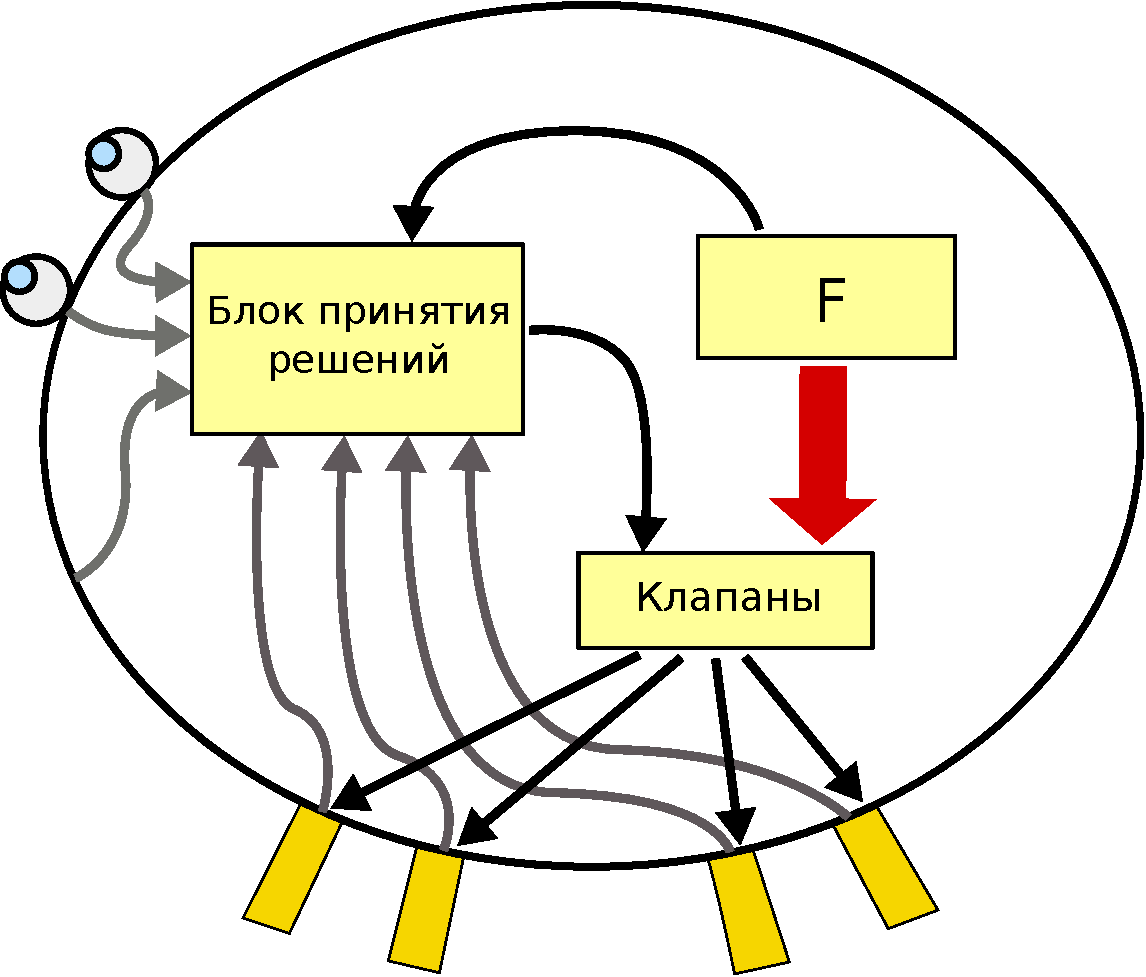
\includegraphics[width=8cm]{figures/creature.pdf}
	\caption{Принципиальная схема машины способной осуществлять выбор.}
\end{figure}

Чтобы система могла осуществлять выбор, она определенным образом сконструирована, как машина. Необходим \textbf{внутренний запас энергии} (F), который может направляться к \textbf{эффекторам}. Чтобы управлять потоком энергии, нужен коммутатор, или \textbf{система клапанов/вентилей}. Распределение потока энергии зависит от внешних и внутренних факторов, нужны \textbf{внешние датчики и индикаторы состояния внутренней среды системы}, например измерение внутреннего запаса энергии.

Механистические компоненты есть в любом организме и некоторых его подсистемах, например, в системе синтеза белка.

\textbf{Конструкция} --- это полный набор степеней свободы статистической системы, не участвующих в тепловом движении в течение времени, интересующего наблюдателя.

\textbf{Применимость понятия <<конструкция>> (<<машина>>) к биологическим системам разной иерархии.}

Для того чтобы понять что следует из такого представления о ключевом, специфическом свойстве живого и об условиях реализации этого свойства --- наличии определенного устройства рассмотрим аналогии между машинами разного рода. Что общего есть, например, у двигателя внутреннего сгорания, фермента, рибосомы и организма. Общее то, что они конструкции, то есть их структура (устройство) не выводится в принципе из законов физики и химии. Отсюда следует, что надежда получить некое общее уравнение биофизики по типу уравнения Шредингера, по-видимому, не имеет оснований. Может ли существовать уравнение магнитофона?

Что, например, можно изучать у живого?
\begin{enumerate}
\item Вопросы оптимального соответствия условиям эксплуатации --- <<принцип адекватной конструкции>>.
\item Поиск ключевых отношений конструкции как целого --- <<принцип биологического эпиморфизма>>.
\textbf{Биологический эпиморфизм} --- свойство общности некоторых черт живых организмов / по Рашевскому
\item Эволюционное возникновение конструкций <<Принцип струк\-тур\-но-функ\-цио\-наль\-но\-го полиморфизма>>
\item Вопросы самосборки, самоформирования и самоподдержания биологических конструкций.
\item Вопросы эффективного накопления и преобразования энергии (механо-химического сопряжения)
\end{enumerate}


\textbf{Методологические замечания}

\begin{enumerate}
\item Иерархия живых систем приводит к относительной независимости от материала и более низкого уровня организации. Например, уравнения, описывающие динамику экосистем не зависят от того из чего сделаны организмы, будут меняться только феноменологические коэффициенты.
\item Способность к выбору не ведет к непредсказуемости поведения (свободе воли) системы, а порождает новые, отличные от физических, закономерности. При этом остается возможность обобщенного описания на уровне ансамблей или типичности.
\end{enumerate}




\newpage
%%%%%%%%%%%%%%%%%%%%%%%%%%%%%%%%%%%%%%%%%%%%%%%%%%%%%%%%%%%%%%%%%%%%%%%%%%%%%%%%%%%%%%%%
\section{Ключевые проблемы абиогенного возникновения жизни и подходы для их снятия}
{\it Невозможность самосборки простейшей живой клетки. Парадокс Кастлера. Эксперименты Миллера-Юри. Необходимые условия для возникновения и эволюции живого. Возможные предшественники живой клетки и химическая эволюция.}

\subsection{Невозможность самосборки простейшей живой клетки}

Получить представление о вероятности случайной сборки бактериальной клетки можно на основе оценки времени, необходимого для перебора всех возможных вариантов не очень длинной полипептидной (белковой) цепи длиной в 100 аминокислотных остатков.

Допустим, что на каждом квадратном нанометре океанской поверхности происходит сборка одного варианта цепи за $10^{-8}$ секунд. Общее количество комбинаций из 20 аминокислот в цепочке длиной 100 равно $20^{100}$ или $\approx 10^{130}$. Площадь Земли составляет примерно $10^{32} \text{нм}^2$. Тогда, для бесповторного перебора всех возможных вариантов комбинаций аминокислот в цепочке потребуется $10^{130} \times 10^{32} \times 10^{-8} = 10^{90}$ секунд. Для сравнения, возраст Вселенной оценивается сейчас величиной $1010$ лет или $\approx 10^{17}$ секунд. Такое чудовищное время потребуется для перебора всех вариантов полипептида с длиной, примерно соответствующей длине инсулина --- не самого большого белка. Жизнедеятельность бактериальной клетки обеспечивается набором из $\approx 1000$ ферментов, то есть белковых макромолекул длиной в среднем 300 аминокислотных остатков. Отсюда следует, что самосборка организма является предельно невероятным событием и, очевидно, жизнь зарождалась по-иному.

\subsection{Парадокс Кастлера}

Случайная самосборка из абиогенных компонентов живой системы сходной по сложности с самыми простыми из известных клеточных организмов имеет ничтожную вероятность и не достойна серьезного рассмотрения \cite{Kastler1967}.

Единственным, соответствующим современным представлениям вариантом происхождения жизни, является постепенное нарастание сложности изначально очень простых систем с сохранением незначительных, а значит и достаточно вероятных изменений системы, которую можно назвать эволюционирующей. Живая клетка является продуктом химической эволюции от существенно более простых молекулярных пребиотических систем.

\subsection{Необходимые условия для возникновения и эволюции живого}

% лекция 23.01.2013
Но жизнь возникла как только охладилась земля, конденсировалась вода... значит путь был другой. Какой?

{\bf Концепция Опарина (1924г).} Живая клетка сформировалась в результате химической эволюции (термин предложил Холдейн) из простых химических конструкций, которые возникали из простых веществ (прекурсоров) самопроизвольно.

Необходимые важнейшие условия для возникновения и эволюции живого:
\begin{itemize}
\item {\bf Фазовая обособленность}. Метаболизм является необходимым условием существования любой формы жизни. Только постоянно используя приток свободной энергии, система может непрерывно обновляться и этим тормозить свое падение в состояние термодинамического равновесия, которое Эрвин Шредингер метко назвал состоянием смерти. Динамический порядок может поддерживаться только за счет постоянной компенсации производства энтропии.

\item {\bf Способность к самовоспроизведению}. Молекулы и специфические упорядоченные структуры, возникшие благодаря межмолекулярным взаимодействиям, имеют ограниченное время жизни из-за теплового движения. Чтобы не потерять накопленную в них информацию, они должны успевать до распада построить хотя бы одну идентичную копию, содержащую план строения и функционирования исходной структуры. Любое биологическое упорядочение направляется информацией.

\item {\bf Мутабельность}. Инструктирование требует специфических взаимодействий. Конечные значения энергий взаимодействия и возмущения, создаваемые тепловыми флуктуациями, делают совершенно точное воспроизведение принципиально невозможным. Всегда существует определенный темп ошибок, или мутаций, --- наличие ошибок --- существенное условие эволюционного прогресса.
\end{itemize}

% лекция 23.01.2013
Тогда проблема самосборки уходит. Проблема Кастлера не устранена. Если мы хотим объяснить возниконовение жизни в той форме, как мы ее знаем, то нам деваться некуда (если подходим с научной позиции), нужно объяснить какая цепочка привела от пробионта к форме жизни, как мы ее знаем. Что детерминирует эволюцию? 1) сами законы физики детерминируют форму жизни (но это мракобесие, законов таких нет) 2) Причины нет, причина, --- сложное взаимодействие различных факторов. Метафора: почему скала Дед возникала именно такой. Поэтому возможны разные варианты жизни --- и мы объясняем только сценарий возникновения жизни.

{\bf Переход от хим эволюции к биологической.}\\
Одни считаю, что вначале появился {\bf метаболизм}, а затем наследование, а другие наоборот, что первой возникла репликация.

Количественное теоретическое рассмотрение динамики биологических систем реакций показывает, что не любой вид самовоспроизведения и мутабельности может привести к возникновению систем, способных к неограниченной эволюции.

Определим живой организм как открытую, саморегулируемую, самовоспроизводящуюся и развивающуюся гетерогенную систему, важнейшими функциональными веществами которой, являются биополимеры --- белки и нуклеиновые кислоты (<<углеводный-шовинизм>>).



\subsection{Эксперименты Миллера-Юри}

Как мы выяснили согласно парадоксу Кастлера случайная самосборка живой клетки невозможна. Необходимо объяснение, каким образом из простейших биологических веществ сформировалась клетка? Откуда они могли взяться, эти вещества?

В определенных условиях сложные биологические вещества могут сформироваться в абиогенных условиях. Исходно думали, что это невозможно. Но Стенли Миллер под руководством Гарольда \'{Ю}ри\footnote{американский физик и физикохимик. Пионер в области исследования изотопов, за открытие одного из которых --- дейтерия --- был награжден Нобелевской премией по химии в 1934 году. Позже перешёл к изучению эволюции планет.} показал, что это не так в своем эксперименте.

Эксперимент М\'{и}ллера-\'{Ю}ри --- один из важнейших экспериментов в исследовании происхождения жизни, в котором симулировались гипотетические условия раннего периода развития Земли для проверки возможности химической эволюции. Фактически это был экспериментальный тест гипотезы, высказанной ранее Опариным и Холдейном, о том, что условия, существовавшие на примитивной Земле, способствовали химическим реакциям, которые могли привести к синтезу органических молекул из неорганических. Был проведен в 1953 году Миллером и \'{Ю}ри. Аппарат, спроектированный для проведения эксперимента, включал смесь газов, соответствующую тогдашним представлениям о составе атмосферы ранней Земли, и пропускавшиеся через нее электрические разряды.

Первичный анализ показал наличие в смеси 5 аминокислот, но более точный повторный анализ, опубликованный в 2008 году \cite{Johnson2008}, показал, что эксперимент привел к образованию 22 аминокислот!

\begin{figure}[ht] \center
 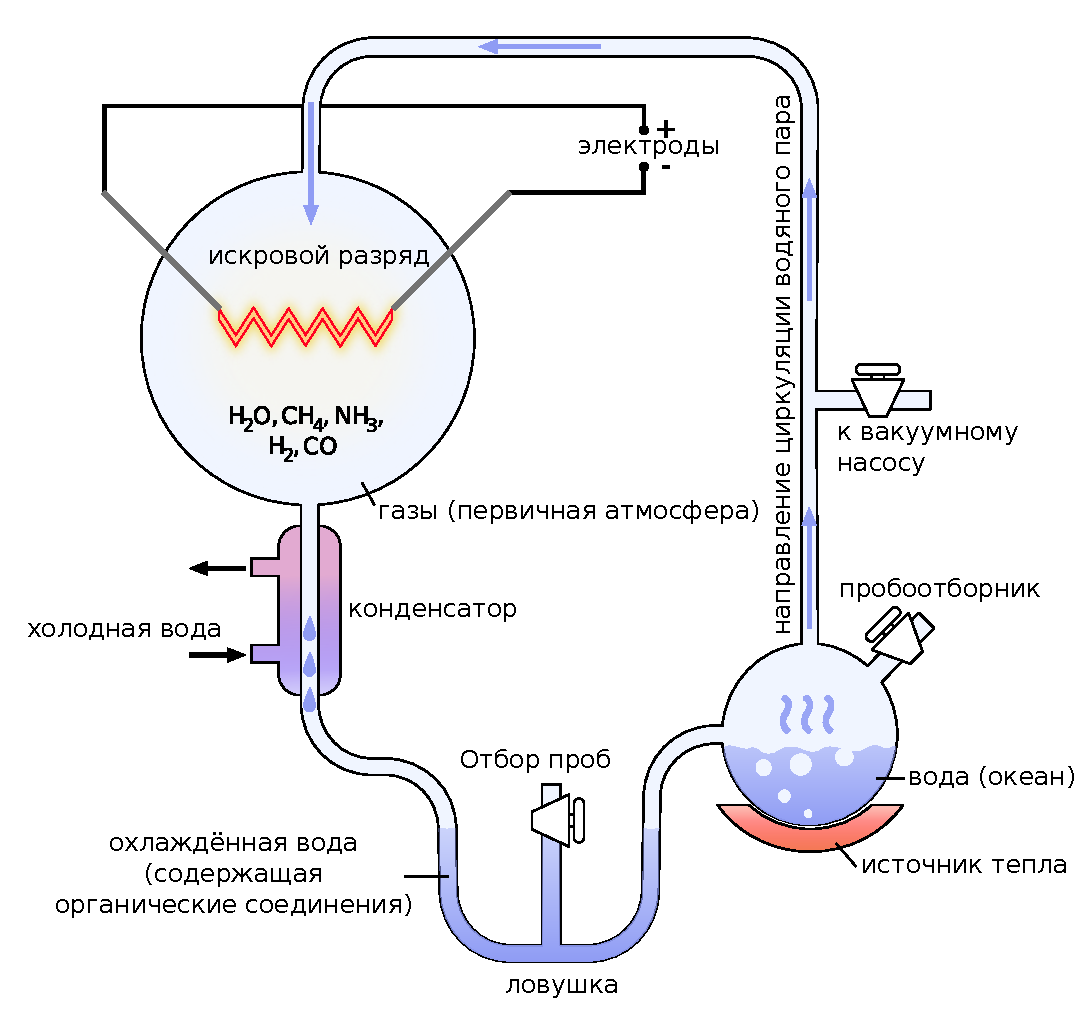
\includegraphics[width=10cm]{figures/fig_2_1.pdf}
 \caption{Схема эксперимента Миллера-Юри}
 \label{miller}
\end{figure}

{\bf Описание эксперимента.} Две колбы, соединенные стеклянными трубками (Рис. \ref{miller}) в цикл. Заполнявший систему газ --- смесь метана ($CH_4$), аммиака ($NH_3$), водорода ($H_2$) и монооксида углерода ($CO$). Одна колба на половину заполнена водой, которая при нагревании испарялась, и пары воды попадали в верхнюю колбу, куда подавались электрические разряды (как молнии на ранней Земле). По охлаждаемой трубке конденсировавшийся пар возвращался в нижнюю колбу, обеспечивая постоянную циркуляцию.

После недели непрерывного цикла Миллер и Юри обнаружили, что десятая часть углерода перешла в органическую форму. Немного углерода оказалось в виде аминокислот, причем глицин оказался наиболее распространенной из них. Были также обнаружены сахар, липиды и предшественники нуклеиновых кислот.

Позже было показано, что даже небольшие изменения условий процесса и состава газовой смеси (например, добавления $N$ или $O$) могли привести к существенным изменениям образующихся органических молекул и эффективности самого процесса их синтеза. В настоящее время вопрос о возможном составе первичной земной атмосферы остается открытым. Однако, считается, что высокая вулканическая активность того времени способствовала выбросу также таких компонентов как диоксид углерода ($CO_2$), азот, сероводород ($H_2S$), двуокись серы ($SO_2$).

{\bf Критика выводов эксперимента.} В эксперименте отсутствует единая хиральность полученных аминокислот, что характерно для аминокислот биологического происхождения. Поэтому дальнейший синтез веществ, лежащих в основе жизни, из полученной смеси затруднен. Хотя синтез важнейших органических веществ был явно продемонстрирован, вывод о возможности химической эволюции, сделанный непосредственно из этого опыта, не вполне обоснован.

%лекция 23.01.2013
{\bf Опыты Фокса, еще получил полипептиды с каталитической активностью... Нужно было нагреть до 800 без доступа кислорода и охладить. Японские исследователи проводят эксеприменты по моделированию подводных гейзеров. Нагрев и охлаждение формируют органические соединения. В космосе тоже есть органика в кристалликах льда.}

Позже было показано, что самореплицирующиеся пептидные системы в состоянии эффективно усиливать молекулы определенного вращения в получаемой смеси, таким образом, преобладание одного из стереоизомеров могло возникнуть естественным образом. Кроме того, показано, что существует возможность спонтанного возникновения хиральности в обычных химических реакциях, известны пути синтеза ряда стереоизомеров, в том числе, углеводородов и аминокислот, в присутствии катализаторов. Впрочем, в эксперименте Миллера-Юри ничего подобного явном виде не произошло.

Если бы даже был получен удачный результат, то в полной мере он не мог бы служить доказательством того, что жизнь на Земле формировалась именно так. Необходимо доказать, что такой сценарий является единственно возможным \cite{Ivanickij2012}.


\subsection{Возможные предшественники живой клетки и химическая эволюция}

Существует гипотеза, согласно которой первые автокаталитические системы (т.н. мультивариантные олигомерные автокатализаторы) развились, когда первые фазовообособленные образования (<<мицеллы>> и пр.) стали аккумулировать простые органические вещества, синтезированные из неорганических. Из простых органических веществ стали формироваться мономеры, а из них --- полимеры, которые стали катализировать синтез один другого, а затем и синтез мономеров из простых веществ.

Один из путей снятия парадокса Кастлера заложен в том, что много структур выполняют одну функцию, значит не структура, а функция выбирается в результате эволюции, и вероятность эффективной эволюции увеличивается. 




\newpage
%%%%%%%%%%%%%%%%%%%%%%%%%%%%%%%%%%%%%%%%%%%%%%%%%%%%%%%%%%%%%%%%%%%%%%%%%%%%%%%%%%%%%%%%
\section{Биосфера --- верхний уровень иерархической организации жизни}
{\it Определение биосферы по Вернадскому. Замкнутость химических и биохимических процессов в биосфере как необходимое условие существования функционирующих автокаталитических систем в конечном объеме в течение неограниченного времени. Парадокс Дарвина-Вернадского и пути его решения.}

\subsection{Определение биосферы по Вернадскому}

Биосфера --- земная оболочка, область существования живого вещества. Она включает в себя не только живые организмы, но и измененную ими среду обитания (кислород в атмосфере, горные породы органического происхождения и т.п.).

Одним из существенных свойств, характеризующих биосферу, является замкнутость потоков веществ в ней. Тогда биосферу можно рассматривать как химический реактор, в который не поступают никакие вещества и не выводятся из него. Химические реакции в таких системах могут протекать неограниченно долго, если в них поступает свободная энергия, а вся совокупность химических реакций носит циклический характер без образования тупиковых продуктов. Можно сказать, что такие системы функционируют, подчиняясь принципу замкнутости. Этот факт впервые ввел в научный обиход В.И.~Вернадский, который постулировал, что жизнь в земной биосфере может существовать неограниченное время и устойчиво развиваться только вследствие циклических превращений веществ, осуществляемых всеми живыми организмами главным образом за счет солнечной энергии. Все, что производит какой-либо организм, в том числе и он сам, потребляется другими организмами и так далее. В биосфере устанавливается непрерывная циклическая сеть химических превращений. Все вещества, входящие в состав биосферы, непрерывно расходуются и образуются вновь; --- правда, разные вещества могут иметь значительно различающиеся скорости оборота. Высокая замкнутость этих процессов означает, что никакие вещества практически не поступают в биосферу и не выносятся из нее в виде тупиковых продуктов и атомы химических веществ биосферы используются живыми организмами многократно в составе самых разных веществ. В результате химических и физических циклических процессов в биосфере устанавливается в среднем относительное постоянство физико-химических параметров среды. Замкнутость является важнейшей интегральной характеристикой биосферы. Сама возможность существования биосферы без длительных изменений ее физико-химических параметров в течение десятков или даже сотен миллионов лет полностью определятся замкнутостью массообменных физико-химических процессов в ней. Хорошо известно, что скорости химических превращений в биосфере таковы, что полное нарушение замкнутости быстро привело бы к ее разрушению. В частности, анализ антарктических кернов показывает, что до 1700 года содержание метана и углекислого газа в атмосфере было практически постоянным в течении, по крайней мере, нескольких предыдущих тысячелетий. Замкнутыми системами с точки зрения происходящих в них физико-химических процессов в большей или меньшей степени являются отдельные экологические системы и даже организмы, но максимальной замкнутостью обладает биосфера. Можно сказать, что принцип замкнутости должен лежать в основе возможности существования в течение неограниченного времени любой системы, основанной на использовании химических процессов, при отсутствии притока веществ в нее и оттока из нее.


\subsection{Замкнутость в биосфере как необходимое условие существования автокаталитических систем}

% лекция 23.01.2013
Биосфера влияет на геологию!!! Живые организмы склонны к неограниченному росту, в силу автокаталитической природы, и всегда испытывают дефицит, быстро перерабатывает и потребляет. Вещества потом возвращаются в цикл. В атмосфере 50(0?) гигатонн углерода. Первичная продукция в древесине 55 гигатонн в год. Был стационар всегда, значит всегда возвращалось. Дыхание почвы!


\subsection{Парадокс Дарвина-Вернадского и пути его решения}

Н.С.~Печуркин высказал... биосфера замкнута, выживают --- больше съесть, меньше умирать. Один и тот же субстрат, тот организм у которого скорость роста выше, тот и выживает. Но организмы не стремятся эту замкнутость сохранить. \textbf{Константа Мано!!!}

Требование замкнутости налагает на процессы, протекающие в системе, определенные ограничения, но эти ограничения до сих пор не изучены и остаются неизвестными. И, неизвестно, какие механизмы обеспечивают замкнутость обмена, поскольку, согласно современным представлениям, эволюция любой популяции определяется прежде всего ее взаимодействием с ближайшим окружением, так что действие отбора, в соответствии с этими представлениями, не находится в прямой связи с замкнутостью обмена веществ в биосфере. Замкнутость обеспечивается всеми организмами в целом и не может быть значимым признаком отбора для отдельной популяции. Эта проблема получила название <<парадокса Дарвина --- Вернадского>>: с одной стороны, живые организмы эволюционируют благодаря взаимодействию со своим ближайшим окружением, с другой же стороны, сохранение замкнутости биосферы требует глобального согласования метаболизма всех живых организмов (или подавляющего большинства). Таким образом, существует необъясненная циклическая замкнутость. Законы биохимии и молекулярной биологии должны быть согласованы с принципом замкнутости, то есть законы микроуровня --- с глобальными законами.

Каким образом достигается это уникальное согласование, мы не знаем!

% лекция 23.01.2013
\textbf{Варианты разрешения}
1. Ограничения материала. 

2. Организмы незаинтересованны в поддержании биосферы, но так как приспособительные свойства ограничены, то автоматически есть предел. За все надо платить. Мухи не защищены, но их много. Улитка растет медленно, но защищена. Мощь хищника оборачивается коротким временем жизни.

3. Рацион не соответствует пропорциям хим состава, поэтому большой поток веществ. Жизнь на разных субстратах. Невозможно возникновения суперхищника.



\chapter{Термодинамика (малых систем)}


%%%%%%%%%%%%%%%%%%%%%%%%%%%%%%%%%%%%%%%%%%%%%%%%%%%%%%%%%%%%%%%%%%%%%%%%%%%%%%%%%%%%%%%%
\section{Классическая термодинамика}
{\it Предмет термодинамики: чем занимается термодинамика. Значение термодинамики для биологии и биофизики. Функции состояния --- язык термодинамики. Начала термодинамики. Температура как функция состояния (нулевое начало). Закон сохранения энергии (первое начало). Энтропия и энергия (второе начало).}
% Осипов А.И. Термодинамика вчера, сегодня, завтра Часть 1. Равновесная термодинамика // Соросовский образовательный журнал. 1999. № 4. С. 79–85.
% Осипов А.И. Термодинамика вчера, сегодня, завтра Часть 2. Неравновесная термодинамика // Соросовский образовательный журнал. 1999. № 5. С. 91–97.

\subsection{Предмет термодинамики: чем занимается термодинамика}

Термодинамика --- это раздел физики, изучающий соотношения и превращения теплоты и других форм энергии. Современную термодинамику принято делить на термодинамику равновесных процессов, квазистатических (классическая термодинамика) и термодинамику неравновесных процессов (термодинамика необратимых процессов). Равновесная термодинамика вводит в рассмотрение новые переменные, такие как внутренняя энергия, температура, энтропия, химический потенциал, а также комбинации перечисленных величин. Все они носят название термодинамических параметров.

\textbf{Классическая (квазистатическая) термодинамика} занимается изучением общих свойств макроскопических систем в состоянии равновесия, а также общих закономерностей, имеющих место при установлении термодинамического равновесия \cite{Osipov1999a}. Термодинамика изучает объекты только в состоянии термодинамического равновесия, под которым подразумевается состояние, в которое с течением времени приходит система, находящаяся при определенных внешних условиях и постоянной температуре окружающих тел. При достижении термодинамического равновесия система <<забывает>> предысторию и <<помнит>> только то, что сохраняется в силу законов сохранения (в изолированной системе это суммарные энергия, импульс и масса). Поэтому время в явном виде в термодинамику не входит. В этом смысле об обычной термодинамике говорят как о термостатике. Поскольку окружающие нас системы, не находятся в состоянии термодинамического равновесия, термодинамическое равновесие есть некая абстракция, упрощенная модель, но в большинстве практически важных случаев она приводит к правильным результатам \cite{Osipov1999a}.

Предметом рассмотрения классической термодинамики служат связи термодинамических параметров друг с другом и с переменными других разделов физики (масса, давление, поверхностное натяжение, сила тока и другие). Химические и фазовые реакции (фазовые переходы первого рода) также есть предмет изучения классической термодинамики, поскольку в этом случае рассматриваются связи между массами компонентов системы и их химическими потенциалами.

\subsection{Значение термодинамики для биологии и биофизики}.

Открытость --- ключевое свойство. Основное свойство --- термодинамическим свойством. И про процессах самоорганизации падение энтропии также термодинамика.

Открытая система может служить абстрактным аналогом живого в целом. Когда мы говорим, что живое --- это открытая система. То это дает универсальность, которое может служить для понимания жизни в целом.

А в частных задачах. Процессы работы мембраны.


\subsection{Функции состояния --- язык термодинамики}

{\bf Функция состояния системы} --- величина, значение которой зависит только от состояния системы, а не от пути, которым оно достигнуто. Функциями состояния являются температура, энергия, энтропия.

Напомним, что основными понятиями классической механики являются координаты
и импульсы составляющих ее частиц. Квантовая механика описывает процессы на языке волновых функций. Термодинамика же разговаривает на языке функций состояния.


Термодинамика работает с функциями состояния, однако среди ее основных понятий имеются два --- работа и теплота, --- которым, вообще говоря, не соответствуют функции состояния. Понятие работы перекочевало в термодинамику из механики и имеет тот же смысл. Работа зависит от истории изменения объема системы. Суммарная работа, совершенная системой при изменении объема от значения $V_1$ до значения $V_2$, равна сумме всех элементарных работ на этом пути:
\begin{equation}
	A = \int_{V_1}^{V_2} p dV
\end{equation}

Термин <<теплота>> исторически остался от несостоявшейся теории теплорода. Термин <<количество теплоты>> не очень удачен. Можно лишь говорить о количестве теплоты, например в калориях, которое подводится к системе вполне определенным образом. Причем количество теплоты, передаваемое телу, будет зависеть от способа подвода.

И работа и количество теплоты не являются полными дифференциалами, поэтому дифференциал этих величин мы везде будем указывать как $\delta A$ и $\delta Q$.


Изолированная система (газ в сосуде с теплоизолирующими стенками) независимо от своего начального состояния в конечном итоге приходит в состояние, которое в дальнейшем уже не меняется. Это конечное состояние называется состоянием теплового равновесия. На микроскопическом уровне материальные частицы продолжают свое сложное движение, но на макроскопическом уровне состояние является простым и определяется несколькими параметрами (температурой, давлением). Если между двумя системами устанавливается физический контакт, то суммарная система приходит в состояние теплового равновесия. Это равновесие не нарушится, если устранить контакт между системами, а затем через некоторое время восстановить его.

Термодинамика исторически возникла как эмпирическая наука об основных способах преобразования внутренней энергии тел для совершения механической работы. Однако в процессе своего развития термодинамика проникла во все разделы физики, химии и биологии, где возможно ввести понятие <<температура>> и позволила теоретически предсказать многие явления задолго до появления строгой теории этих явлений.


\subsection{Начала термодинамики}

\subsection{Температура как функция состояния (нулевое начало)}

{\bf 0. Нулевое начало термодинамики} постулирует существование термодинамического равновесия и вводит понятие абсолютной температуры.

{\bf Термодинамическое равновесие}. Для каждой изолированной термодинамической системы существует состояние термодинамического равновесия, которого она при фиксированных внешних условиях с течением времени самопроизвольно достигает. Если две изолированные системы $A$ и $B$ приведены в контакт друг с другом, то после достижения термодинамического равновесия полной системой $A+B$ системы $A$ и $B$ находятся в состоянии теплового (термического) равновесия друг с другом. При этом каждая из систем $A$ и $B$ в отдельности также находится в состоянии термодинамического равновесия. Это равновесие не нарушится, если устранить контакт между системами, а затем восстановить его. Следовательно, если установление контакта между двумя системами $A$ и $B$, которые до этого были изолированными, не приводит ни к каким изменениям, то эти системы находятся в тепловом равновесии друг с другом.

{\bf Закон транзитивности теплового равновесия}. Если системы $A$ и $B$ находятся в тепловом равновесии и системы $B$ и $C$ находятся в тепловом равновесии, то системы $A$ и $C$ также находятся в тепловом равновесии между собой. На основании этого закона делается вывод о существовании абсолютной температуры как термодинамического параметра, обладающего свойствами эмпирической температуры, но не зависящего от способа ее измерения. Равенство температур есть условие теплового равновесия систем (или частей одной и той же системы).

Состояние каждой из систем $A$, $B$ и $C$ характеризуется давлением $p$ и объемом $V$. Когда мы говорим, что между двумя системами существует равновесие, то это значит, что объем и давление одной системы связаны с объемом и давлением другой системы. Таким образом, для трех систем в равновесии существуют три функциональных соотношения \cite{Osipov1999a}:
\begin{equation}
	\begin{aligned}
		F_1 (p_A, V_A, p_B, V_B) = 0, \\
		F_2 (p_A, V_A, p_C, V_C) = 0, \\
		F_3 (p_C, V_C, p_B, V_B) = 0.
	\end{aligned}
\end{equation}

Эти соотношения удовлетворяются, если каждую функцию представить в виде: 
\begin{equation}
	\begin{aligned}
		F_1 = f_A (p_A, V_A) - f_B (p_B, V_B),\\
		F_2 = f_A (p_A, V_A) - f_C (p_C, V_C),\\
		F_3 = f_B (p_B, V_B) - f_C (p_C, V_C).
	\end{aligned}
\end{equation}

Если теперь одну из систем, например $A$, использовать как термометр, то значение функции $f_A (p_A, V_A) = \Theta$ можно рассматривать как эмпирическую температуру. Сами же уравнения:
\begin{equation}
	f_A(p_A, V_A)=f_B(p_B, V_B)=f_C(p_C, V_C)=\Theta,
\end{equation}
называются уравнениями состояния. В случае идеального газа это уравнение Менделеева-Клапейрона:
\begin{equation}
	\label{mendeleev}
	P V = \nu R T
\end{equation}

\subsection{Закон сохранения энергии (первое начало)}

{\bf 1. Первое начало}.
Каждая термодинамическая система обладает характеристической функцией состояния --- энергией. Эта функция состояния возрастает на величину сообщенного системе тепла $\delta Q$ и уменьшается на величину совершенной системой внешней работы $\delta A$. Для изолированной системы справедлив закон сохранения энергии \cite{Osipov1999a}.

Первое начало термодинамики можно записать в виде:
\begin{equation}
	d U = \delta Q - \delta A \qquad \text{или} \qquad \delta Q = d U + \delta A,
\end{equation}
где $d U$ --- внутренняя энергия, характеристическая функция состояния. Внутренняя энергия включает энергию хаотического (теплового) движения всех микрочастиц системы (молекул, атомов, ионов и т.д.) и энергию взаимодействия этих частиц.

Для изолированной системы, то есть для системы, не обменивающейся с окружающей средой ни веществом, ни энергией $dU = 0$ и, следовательно, $U = const$, то есть имеет место закон сохранения энергии.

В циклическом процессе внутренняя энергия не изменяется:
\begin{equation}
	\oint d U = 0 \Rightarrow \oint \delta Q - \oint \delta A
		= 0 \Rightarrow \oint \delta Q = \oint \delta A
\end{equation}

Откуда очевидно, что совершение работы без подвода теплоты невозможно. Поэтому первое начало термодинамики часто формулируют как невозможность существования вечного двигателя первого рода, который совершал бы работу, не черпая энергию из какого-либо источника.

\textbf{Манипуляции надо доделать, не понятно!!!}

$U = U(V, T)$ --- характеристическая функция состояния, теплота --- неполный дифференциал:
\begin{equation}
	\label{eq316.1}
\left. \begin{aligned}
\delta Q =dU + p\,dV\\
dU = \left( \frac{\partial U }{\partial T} \right)_{\!\! V} \!\!\! dT + \left( \frac{\partial U }{\partial V} \right)_{\!\! T} \!\!\! dV 
\end{aligned}
\right\rbrace \Rightarrow \delta Q = \left( \frac{\partial U }{\partial T} \right)_{\!\! V} \!\! dT + \left[\! \left( \frac{\partial U }{\partial V} \right)_{\! T}\!\!\! + p \right] \! dV
\end{equation}

Вспомним об одном свойстве уравнений в полных дифференциалах. Уравнение вида:
\begin{equation}
	F (x,y) dx + G (x,y) dy = 0,
\end{equation}
называется уравнением в полных дифференциалах тогда и только тогда, если справедливо равенство:
\begin{equation}
	\frac{\partial F (x,y)}{\partial y} = \frac{\partial G (x,y)}{\partial x}
\end{equation}

Воспользуемся этим свойством в обратном порядке. Допустим, что нет подвода теплоты ($\delta Q = 0$), тогда уравнение (\ref{eq316.1}) является уравнением в полных дифференциалах и справедливо:
\begin{equation}
	\frac{\partial}{\partial V} \left( \frac{\partial U}{ \partial T}\right)_{\! V} = 
	\frac{\partial}{\partial T} \left[
			\left( \frac{\partial U}{ \partial V}\right)_{\! T} + p
		\right],
\end{equation}
но $\left( \frac{\partial p}{ \partial T}\right)_{\! V} \not = 0$, что еще раз доказывает невозможность вечного двигателя первого рода (невозможно совершения работы без подвода теплоты).


\subsection{Энтропия и энергия (второе начало)}

Для начала введем необходимые определения для процессов и систем:
\begin{itemize}
\item\textbf{Обратимым термодинамическим процессом} называется термодинамический процесс, допускающий возможность возвращения системы в первоначальное состояние без того, чтобы в окружающей среде остались какие-либо изменения. Необходимым и достаточным условием обратимости термодинамического процесса является его равновесность.
\item\textbf{Стационарное состояние системы} называется равновесным, если его неизменность во времени не обусловлена протеканием какого-либо внешнего по отношению к системе процесса.
\item\textbf{Равновесным процессом} называется процесс, при котором система проходит непрерывный ряд равновесных состояний.
\item\textbf{Необратимым термодинамическим процессом} называется термодинамический процесс, не допускающий возможности возвращения системы в первоначальное состояние без того, чтобы в окружающей среде остались какие-либо изменения.
\item\textbf{Все реальные процессы} протекают с конечной скоростью. Они сопровождаются трением, диффузией и теплообменом при конечной разности между температурами системы и внешней среды. Следовательно, все они \textbf{неравновесны и необратимы}.
\end{itemize}

{\bf Второе начало термодинамики}. Каждая термодинамическая система обладает функцией состояния, называемой энтропией. Энтропия вычисляется следующим образом: система переводится из произвольно выбранного начального состояния в соответствующее конечное состояние через последовательность состояний равновесия; вычисляются все подводимые при этом к системе порции тепла $\delta Q$, каждая делится на соответствующую ей абсолютную температуру $T$, и все полученные таким образом значения суммируются. При реальных (неравновесных) процессах энтропия изолированной системы возрастает.

Если обозначить энтропию через $S$, то из этого определение следует, что приращение энтропии:
\begin{equation}
	d S = \frac{Q}{dT}
\end{equation}
Если подставить таким образом определенную энтропию в выражение для первого начала термодинамики, то получится соотношение
\begin{equation}
	d U = T dS + \delta A,
\end{equation}
которое известно в литературе как соотношение Гиббса. Это фундаментальное уравнение объединяет первое и второе начала, и в нем по существу заключена вся равновесная термодинамика.

%Теорема Карно: термический КПД () обратимого цикла Карно не зависит от природы рабочего тела и является функцией только абсолютной температур нагревателя ($T_1$) и холодильника ($T_2$):
%
%Для обратимого цикла: 

Некоторые из формулировок второго начала термодинамики:
\begin{itemize}
\item[A.] Постулат Томсона (Кельвина): невозможен процесс, единственным результатом которого является совершение работы, эквивалентной количеству теплоты, полученному от нагревателя;
\item[B.] Постулат Клаузиуса: невозможен процесс, единственным результатом которого является передача энергии в форме тепла от холодного тела к горячему;
\item[C.] вечный двигатель второго рода невозможен.
\end{itemize}

Энтропия физической однородной системы является функцией двух независимых параметров состояния, например $p$ и $T$ или $T$ и $V$ (масса системы предполагается неизменной).
\begin{equation}
	\left\lbrace
	\begin{aligned}
		S (V, T) & = \int_0^T C_V \frac{dT}{T} + S_0\\
		S (p, T) & = \int_0^T C_p \frac{dT}{T} + S_0
	\end{aligned}
	\right.
\end{equation}

Откуда получаем:
\begin{equation}
	S_2 - S_1 = \int_1^2 \frac{\delta Q}{T_\text{обр}},
\end{equation}
--- изменение энтропии в любом обратимом процессе:


	– математическая запись второго начала.


Неравенство Клаузиуса, как математическая запись второго начала термодинамики для необратимых процессов в неизолированной системе:

Для обратимых процессов справедливо равенство Клаузиуса:


Основное соотношение термодинамики (соотношение Гиббса):
Для обратимых процессов

Для необратимых процессов

% энтропия приводит в движение открытые системы, <<крутит шестеренки>>




\newpage
%%%%%%%%%%%%%%%%%%%%%%%%%%%%%%%%%%%%%%%%%%%%%%%%%%%%%%%%%%%%%%%%%%%%%%%%%%%%%%%%%%%%%%%%
\section{Второе начало термодинамики и развитие биологических систем}
{\it Энтропия и биологические системы. Химическое сродство. Функция диссипации. Производство энтропии в биологических системах.}

\subsection{Энтропия и биологические систем}

\textbf{Второй закон термодинамики в открытых (биологических) системах}

Критерием направления самопроизвольных изменений в изолированной системе служит увеличение энтропии $S$, а конечным состоянием --- состояние равновесия. В то же время открытые системы, в первую очередь биологические, прекращают свое функционирование как таковые в состоянии равновесия.

В термодинамическом отношении открытые (биологические) системы в процессе своего изменения проходят через ряд неравновесных состояний, что, в свою очередь, также сопровождается соответствующими изменениями термодинамических переменных.

В целом поддержание неравновесных состояний в открытых системах возможно лишь за счет создания в них соответствующих потоков вещества и энергии.

При обратимых процессах изменение энтропии равно нулю, а при необратимых оно положительно. Таким образом, чем меньше в системе градиенты энергии и чем больше в ней рассеянной в виде тепла деградированной энергии, тем больше ее энтропия.

При \textbf{необратимом процессе} система изменяется по направлению к конечному состоянию (при самопроизвольном протекании процесса --- к состоянию равновесия) с определенной скоростью. При этом часть свободной энергии системы теряется в виде тепла. Эти потери и характеризует энтропия. \textbf{Обратимый процесс} --- это такой, при котором система в каждый момент времени находится в состоянии, бесконечно близком к термодинамическому равновесию, и достаточно лишь незначительно изменить условия, чтобы процесс был обращен.

Таким образом, открытым системам присущи неравновесные состояния, параметры и свойства которых, вообще говоря, есть функции времени. Для термодинамического потенциала $G$ и свободной энергии $F$ это означает, что $G = G(T,p,t)$, $F = F(T,v,t)$.

\textbf{Изменение энтропии открытой системы.} Оно может происходить либо за счет процессов обмена системы с внешней средой ($d_eS$), либо за счет возникновения энтропии в самой системе вследствие внутренних необратимых изменений ($d_iS$). Постулируется, что общее изменение энтропии открытой системы ($dS$) складывается из двух независимых частей:
\begin{equation}
	\label{dS}
	dS = d_e S + d_i S.
\end{equation}

В этом состоит исходное положение термодинамики необратимых процессов. 

Если внутри системы протекают обратимые изменения, то они не сопровождаются возникновением энтропии и $d_iS = 0$. Во всех случаях необратимых изменений $d_iS > 0$. Очевидно, для изолированных систем, где $d_eS = 0$, выражение (\ref{dS}) сводится к: 
\begin{equation}
	dS = d_i S > 0,
\end{equation}
что соответствует классической формулировке второго закона термодинамики для изолированных систем.

Если в каком-либо участке открытой системы одновременно протекают различные необратимые процессы, то величина $d_iS > 0$ описывает приращение энтропии, являющееся следствием взаимодействия этих необратимых процессов друг с другом.

Именно разделение величины изменения энтропии открытой системы на две составляющие $d_eS$ и $d_iS$ позволяет изучать различия в термодинамических свойствах открытых и изолированных систем.

Продифференцируем выражение (\ref{dS}): 
\begin{equation}
	\label{dSdt}
	\frac{dS}{dt} = \frac{d_eS}{dt} + \frac{d_iS}{dt}.
\end{equation}

Полученное уравнение означает, что скорость изменения энтропии системы $d_eS /dt$ равна скорости обмена энтропией между системой и окружающей средой плюс скорость возникновения энтропии внутри системы.

Член $d_eS /dt$, учитывающий процессы обмена системы со средой, может быть и положительным, и отрицательным, так что при $d_iS /dt > 0$ общая энтропия системы может как возрастать, так и убывать.

Положительная величина $d_eS /dt > 0 $ связана с увеличением энтропии системы в результате обмена веществом и энергией с внешней средой. Отрицательная величина $d_eS /dt < 0$ соответствует тому, что отток положительной энтропии от системы во внешнюю среду превышает приток положительной энтропии извне, так что в результате общая величина баланса обмена энтропией между системой и средой является отрицательной. Очевидно, что при одном и том же условии $d_iS /dt > 0$ возможны следующие три случая:

1) $dS/dt > 0$,		если $d_eS / dt> 0$ 	или если $d_eS / dt$ < 0,	но $|d_eS / dt| < d_iS /dt$;\\
2) $dS/dt < 0$,		если $d_eS / dt < 0$		и $|d_eS / dt| > d_iS /dt$;\\
3) $dS/dt = 0$,		если $d_eS / dt < 0$		и $|d_eS / dt| = d_iS /dt$.

Последний случай соответствует установлению в системе стационарного состояния, при котором продуцирование энтропии в системе $d_iS /dt$ компенсируется оттоком положительной энтропии во внешнюю среду, так что общее изменение энтропии равно нулю:
\begin{equation}
	\label{dSdt0}
	dS = d_e S + d_i S = 0 \qquad dS/dt = d_e S / dt + d_i S / dt = 0.
\end{equation}

Анализ общих свойств биологических систем на основе уравнения (\ref{dSdt}) помог объяснить внешнее противоречие между поведением организмов и вторым законом классической термодинамики. Действительно, рост и развитие организмов сопровождаются усложнением их организации и с точки зрения классической термодинамики выглядят как самопроизвольное уменьшение энтропии живых систем, что, конечно, явно противоречит второму закону. Однако это противоречие лишь кажущееся, поскольку направление самопроизвольных процессов определяется увеличением энтропии лишь для изолированных систем, а отнюдь не для открытых, какими являются биологические системы.

\textbf{В реальных условиях развитие организмов, сопровождающееся уменьшением общей величины их энтропии, происходит при условии:}
\begin{equation}
	d_e S dt < 0, \qquad d_e S dt > d_i S dt,
\end{equation}
за счет того, что в других участках внешней среды идут сопряженные процессы с образованием положительной энтропии.

Общий энергообмен земных организмов можно упрощенно представить как образование в фотосинтезе сложных молекул углеводов из $CO_2$ и $H_2O$ с последующей деградацией продуктов фотосинтеза в процессах дыхания. Именно этот энергообмен обеспечивает существование и развитие как отдельных организмов --- звеньев в круговороте энергии, так и в жизни на Земле в целом. С этой точки зрения, уменьшение энтропии живых систем в процессах их жизнедеятельности обусловлено в конечном итоге поглощением квантов света фотосинтезирующими организмами, что, однако, с избытком компенсируется образованием положительной энтропии в ядерных реакциях на Солнце. Этот принцип относится и к отдельным организмам, для которых поступление извне питательных веществ, несущих приток <<отрицательной>> энтропии, всегда сопряжено с продуцированием положительной энтропии при их образовании в других участках внешней среды, так что суммарное изменение энтропии в системе организм + внешняя среда всегда положительно. Точно так же уменьшение энтропии в части клетки, где идет биохимический синтез, происходит за счет избыточного увеличения энтропии в других частях организма или среды.

В целом уменьшение энтропии живых систем в процессе их роста происходит за счет свободной энергии, освобождаемой при распаде поглощаемых извне питательных веществ или за счет энергии солнца (фотосинтез). Одновременно это приводит к увеличению их свободной энергии. Таким образом, поток отрицательной энтропии необходим для компенсации процесса возникновения положительной энтропии и убыли свободной энергии в клетке в результате самопроизвольных реакций метаболизма. В сущности, речь идет о круговороте и превращениях свободной энергии, за счет которой поддерживается функционирование живых структур. 

\textbf{Вычисление величины $d_iS$.}

В открытых системах, где протекают процессы, приводящие к изменению химического состава веществ, вычисление $d_iS$ представляет собой главную проблему. Если внутри открытой системы достигнуто равновесие в отношении распределения температуры (но не химического состава реагентов) и процессы обмена со средой протекают равновесно, такая система находится в частично равновесном состоянии. Общее изменение энтропии для нее составит:
\begin{equation}
	dS = d_e S + d_i S = 0,
\end{equation}
где $d_e = \delta Q/T$ описывает изменение энтропии открытой системы в результате ее равновесного теплообмена с окружающей средой, а член $d_iS$ соответствует самопроизвольному возрастанию энтропии внутри системы за счет химических превращений веществ, находившихся в начальном неравновесном состоянии, и совершению при этом полезной работы.
Отсюда следует, что:
\begin{equation}
	\label{eq.205}
	d_i S = d S - d_e S = dS - \delta Q / dt.
\end{equation}

Так как поглощенная теплота приводит только к совершению механической работы, а вся полезная работа $\delta A'_{max}$ в системе совершается за счет внутренних самопроизвольных химических реакций, то первый закон термодинамики имеет вид:
\begin{equation}
	\label{eq.206}
	\delta Q = dU + pdv
\end{equation}

Подставляя в (\ref{eq.205}) выражение (\ref{eq.206}), получим, что:
\begin{equation}
	\label{eq.207}
	d_i S = (1/T) (TdS - dU - pdV).
\end{equation}

Так как:
\begin{equation}
	\label{eq.208}
	dG = -TdS + dU + pdV, \qquad \text{то:}
\end{equation}
\begin{equation}
	d_i S = - dG / T, \qquad (T, p = const).
\end{equation}

Таким образом, скорость возникновения энтропии в открытой системе при постоянных температуре и давлении пропорциональна скорости уменьшения ее термодинамического потенциала:
\begin{equation}
	\frac{d_i S}{dt} = - \frac 1 T \frac{dG}{dt} =
		- \frac 1 T \sum_k \mu _k \left( \frac{dn_k}{dt} \right).
\end{equation}

В соответствии с ранее сделанным предположением в частично равновесной системе единственной причиной необратимости, а значит, уменьшения ее термодинамического потенциала ($-dG < 0$) и увеличения энтропии ($d_iS > 0$) являются химические реакции, самопроизвольное протекание которых приводит к изменению химического состава системы и соответствующему совершению полезной работы.

\begin{equation}
	\left.
	\begin{aligned}
		\frac{d_i S}{dt} & = - \frac 1 T \frac{dG}{dt} = - \frac 1 T \sum_k \mu _k \left( \frac{dn_k}{dt} \right)\\
		d n_k & = v_k d \xi
	\end{aligned}\right\rbrace
	\quad \Rightarrow \quad
	\frac{d_i S}{dt} = - \frac{1}{T} \sum_k \mu_k v_k \frac{d \xi}{dt} = - \frac{1}{T} A v,
\end{equation}
где $\mu_k$, $v_k$ --- соответственно химический потенциал и стехиометрический коэф. $k$-го реагента.
\begin{equation}
	\frac{d_i S}{dt} = \int \sigma dV \ge 0,
\end{equation}
где $\sigma = A v/ T$ --- функция диссипации $\sigma = \frac{1}{T} \sum_l A_l v_l \ge 0$. 

Изолированные реакции невозможны, если $A_j v_j < 0$.
\begin{equation}
	\sigma = \sum_l J_l X_l,
\end{equation}
где $X_l$ --- обобщенные силы $A/T$,\\
$J_l$ --- обобщенный поток $v$.

В линейном приближении: 
\begin{equation}
	J_i = \sum_{k=1}^n L_{ik}^k,
\end{equation}

Вблизи равновесия по теории Онзагера $L_{ij} = L_{ji}$:

\begin{multline}
	\left.
	\begin{aligned}
		J_1 & = L_{11}X_1 + L_{12}X_2\\
		J_2 & = L_{21}X_1 + L_{22}X_2
	\end{aligned}\right\rbrace \quad \Rightarrow \\
	\sigma = L_{11}X_1^2 + ( L_{12} + L_{21})X_1 X_2 + L_{22}X_2^2 \ge 0 \quad \Rightarrow\\
	 L_{11} > 0, \qquad L_{22} > 0, \qquad L_{12} < L_{11} L_{22}
\end{multline}

Знак $L_{12}$ может быть любым.


В биологических системах особое значение имеет нарушение пространственной симметрии и возникновение диссипативных структур, как самопроизвольный переход от однородного стационарного состояния к пространственно неоднородному.





\newpage
%%%%%%%%%%%%%%%%%%%%%%%%%%%%%%%%%%%%%%%%%%%%%%%%%%%%%%%%%%%%%%%%%%%%%%%%%%%%%%%%%%%%%%%%
\section{Теория Онзагера}
{\it Принцип локальности. Термодинамические уравнения движения. Соотношение взаимности. Сопряжение химических процессов с механохимическими процессами и активным переносом через мембраны.}
% Осипов А.И. Термодинамика вчера, сегодня, завтра Часть 2. Неравновесная термодинамика // Соросовский образовательный журнал. 1999. № 5. С. 91–97.


\subsection{Принцип локальности}


\subsection{Термодинамические уравнения движения}

Работа фермента тоже есть механо-химический процесс.

\subsection{Соотношение взаимности.}
Все взаимосвязано 


Источником энтропии в открытых (биологических) системах служат потоки превращения химических веществ, поэтому соотношение между значениями движущих сил и скоростей процессов играет важную роль в термодинамике биологических систем. Обозначим через значение движущих сил, а через --- значение потока, или суммарной скорости соответствующего потока. Очевидно, что во всех случаях возрастание энтропии имеет вид:
,	(21.1)
где --- движущая сила, --- величина потока.

Соотношения Онзагера. Если открытая система находится вблизи термодинамического равновесия, когда значения движущих сил весьма малы, а сами процессы протекают достаточно медленно ($J \approx 0$), то и связаны следующим соотношением:
,	(21.2)
где --- постоянный, или линейный, коэффициент.

Справедливость соотношений (21.2) подтверждается, например, законом Ома, где значение потока электричества пропорционально движущей силе --- разности потенциалов , a --- линейный коэффициент пропорциональности . Для химических процессов, когда скорости прямой и обратной реакций почти равны между собой, также справедливо выражение:.
где --- суммарная скорость процесса, равная разности скоростей прямой и обратной реакций.
Особый интерес представляет случай, когда в системе одновременно протекает несколько процессов, каждый из которых характеризуется собственными значениями скорости и движущей силы. Эти процессы могут взаимодействовать друг с другом так, что скорость каждого из них будет зависеть и от движущих сил всех других процессов. Для двух взаимодействующих процессов это запишется следующим образом:
	(21.3)
где коэффициенты взаимности Онзагера соответствуют возможной взаимосвязи потоков.
Соотношения типа (21.3) применимы, например, в случае одновременной диффузии вещества и переноса теплоты или переноса электрического тока и диффузии ионов. Вблизи равновесия:
 	(21.4)
Это так называемое соотношение взаимности Онзагера показывает, что если поток 1-го необратимого процесса испытывает влияние сродства необратимого 2-го процесса через посредство коэффициента, то и поток 2-го процесса также испытывает влияние сродства через посредство того же самого коэффициента .
В общем случае, когда в системе одновременно протекает K процессов,

 , где $\beta$ --- скорость продуцирования энтропии
где, при откуда следует: 	(21.5)

В выражении (21.5) силы подбираются таким образом, чтобы размерности правых и левых частей совпадали [Дж с-1]. Соотношения Онзагера играют важную роль в термодинамике необратимых процессов и, кроме того, находят непосредственное использование в анализе свойств биологических систем. Так, используя эти соотношения, можно, определяя значения коэффициентов , установить количественную связь между одновременно протекающими в клетке процессами.






\newpage
%%%%%%%%%%%%%%%%%%%%%%%%%%%%%%%%%%%%%%%%%%%%%%%%%%%%%%%%%%%%%%%%%%%%%%%%%%%%%%%%%%%%%%%%
\section{Стационарные состояния в неравновесных системах}
{\it Производство энтропии. Теорема Пригожина о минимальном производстве энтропии в стационарном состоянии, близком к равновесию. Термодинамика и биологическая эволюция.}
% Осипов А.И. Термодинамика вчера, сегодня, завтра Часть 2. Неравновесная термодинамика // Соросовский образовательный журнал. 1999. № 5. С. 91–97.

\subsection{Производство энтропии}

Производство энтропии базируется на соотношение взаимности.

с 22 и 15 вопросом.

Неравновесная термодинамика не получила развития поскольку надо говорить о кинетике.


Из теории Онзагера вытекает теорема Пригожина о минимальности производства энтропии.

Рассмотрим открытую систему, в которой одновременно протекают необратимые процессы (вблизи состояния термодинамического равновесия, где справедливы линейные соотношения между значениями скоростей и сродства и соотношения взаимности Онзагера.

Пусть в стационарном состоянии . В случае химической реакции это означает, что в стационарном состоянии изменение концентрации соответствующего промежуточного вещества не происходит во времени.


При :

Если система близка к равновесию, то из соображений теории Онзагера, тогда:

В стационарном состоянии, близком к равновесию продукция минимальна.

Рис. V.2 Скорость продуцирования энтропии около стационарной точки: 
I --- зависимость величины от движущих сил около стационарной точки х1 ; II– зависимость от времени величины $\beta$ (1,3) и $\beta$(2) при приближении к стационарному состоянию вблизи равновесия (вертикальная пунктирная линия соответствует моменту перехода системы в стационарное состояние)

На рис. V.2 представлены в виде графиков полученные выводы. Неравенства (7) одновременно приводят к выводу и об устойчивости стационарных состояний. Действительно, если система находится в стационарном состоянии, то она не может самопроизвольно выйти из него за счет внутренних необратимых изменений. Если же в результате флуктуации система незначительно удаляется от стационарного состояния, то в силу (7) в ней должны произойти такие внутренние изменения, которые вновь возвратят ее к исходному стационарному состоянию (рис. V.2). 
Это и означает, что данное стационарное состояние является устойчивым, а возвращение в него при незначительных возмущениях аналогично проявлению известного принципа Ле-Шателье --- устойчивости равновесных состояний. Очевидно, условие устойчивости стационарного состояния имеет вид $d \beta > 0$. (8) 

Знак положительного неравенства показывает, что любое отклонение от устойчивого стационарного состояния вызовет увеличение скорости продуцирования энтропии.
Стационарное состояние, к которому может эволюционировать открытая система, заведомо является неравновесным состоянием, в котором диссипативные процессы происходят с ненулевыми скоростями. Но все величины, описывающие систему (температура, концентрация и др.), перестают в нём зависеть от времени. Не зависит от времени в стационарном состоянии и энтропия системы. В разделе <<Характеристика производства энтропии>> было показано, что в стационарном состоянии производство энтропии неравновесных систем компенсируется отрицательным потоком энтропии из внешней среды:

То есть, стационарность диссипативных процессов в системе поддерживается постоянным потоком извне вещества и энергии.

Под устойчивостью стационарного состояния физико-химической системы понимают её невосприимчивость к случайным флуктуациям, то есть случайным кратковременным изменениям значений управляющих параметров системы (концентраций компонентов, температуры окружающей среды, скорости протока реагентов через реактор и т.п.). Если стационарное состояние системы является устойчивым, то случайные флуктуации не будут оказывать существенного воздействия на поведение системы. Если же стационарное состояние неустойчиво, тогда под воздействием случайных флуктуаций система самопроизвольно перейдёт в качественно новое состояние.
Для исследования устойчивости систем существует два метода, разработанных русским математиком А.М. Ляпуновым. Первый метод Ляпунова основан на определении корней характеристического уравнения системы дифференциальных уравнений, описывающей физико-химическую систему (подробно он будет рассмотрен во второй части курса в разделе <<Методы исследования линейных систем>>). Второй метод Ляпунова основан на исследовании физико-химической системы с помощью функции Ляпунова.

Определение. Рассмотрим некоторое стационарное состояние системы . Если найдётся функция , которая равна нулю в стационарном состоянии
 и знакоопределена в его окрестности, т.е.
 или то такую функцию называют функцией Ляпунова.
Второй метод Ляпунова заключается в исследовании знака производной от функции Ляпунова dV/dt. Если в окрестности рассматриваемого стационарного состояния знак функции Ляпунова V отличается от знака её производной dV/dt, то такое стационарное состояние устойчиво; если же знаки функции Ляпунова V и её производной dV/dt совпадают, то стационарное состояние неустойчиво: 
 или  состояние устойчиво;
 или  состояние неустойчиво.
В стационарном состоянии концентрации промежуточных продуктов перестают изменяться со временем, что достигается при определенных соотношениях между скоростями различных химических процессов, ответственных за образование и распад промежуточных соединений. В открытой системе суммарное изменение энтропии в стационарном состоянии равно нулю: dS = deS + diS = 0. Однако при этом члены deS и diS, соответствующие процессам обмена системы с окружающей средой и внутренним необратимым процессам внутри системы, отличны от нуля. Возникает вопрос: каким образом изменение энтропии за счет самопроизвольных необратимых процессов внутри открытой системы связано с установлением в ней стационарного неравновесного состояния? Иными словами, можно ли по характеру изменения во времени величины diS/dt, предсказать установление в открытой системе стационарного состояния? В такой постановке эта проблема сходна с проблемой классической термодинамики о предсказании направления самопроизвольных необратимых процессов в изолированной системе на основе характера изменения ее всегда идут в направлении увеличения энтропии, которая достигает своего максимального значения в конечном равновесном состоянии.








\newpage
%%%%%%%%%%%%%%%%%%%%%%%%%%%%%%%%%%%%%%%%%%%%%%%%%%%%%%%%%%%%%%%%%%%%%%%%%%%%%%%%%%%%%%%%
\section{Термодинамические потенциалы}
{\it Основное соотношение термодинамики (соотношение Гиббса). Свободная энергия. Энтальпия. Термодинамический потенциал Гельмгольца. Термодинамический потенциал Гиббса. Вычисление энтропии.}

\subsection{Основное соотношение термодинамики (соотношение Гиббса)}

\subsection{!!! Вывод термодинамического потенциала}

\begin{equation}
	\delta Q = d U + p dV
\end{equation}

\begin{equation}
	d S = \frac{\delta Q}{T}
\end{equation}


\begin{equation}
	TdS dU + p dV
\end{equation}


\begin{equation}
	d U = T dS - p dV + \delta A*
\end{equation}

И тут понятно, что если условия


{\bf Характеристической функцией} называется функция состояния системы, посредством которой, а также ее производных могут быть явно выражены термодинамические свойства системы.

{\bf Термодинамическим потенциалом} называется характеристическая функция, убыль которой в равновесном (обратимом) процессе, протекающем при неизменных значениях определенной пары термодинамических параметров ($T$, $V$, $p$, $S$), равна --- полной работе, произведенной системой, за вычетом работы против внешнего давления:

.	(7.1)
 --- величина максимальной полезной работы за вычетом работы против сил внешнего давления.

Вывод 


\textbf{Энтальпия} (также тепловая функция и теплосодержание) --- термодинамический потенциал, характеризующий состояние системы в термодинамическом равновесии при выборе в качестве независимых переменных давления, энтропии и числа частиц.
, где --- давление, а --- объем.

Поскольку в изобарном процессе работа равна , приращение энтальпии в квазистатическом изобарном процессе равно количеству теплоты, полученному системой.

Свободная \textbf{энергия Гельмгольца} (также просто свободная энергия) --- термодинамический потенциал, убыль которого в квазистатическом изотермическом процессе равна работе, совершенной системой над внешними телами. 
, где --- температура и --- энтропия.

Поскольку в изотермическом процессе количество теплоты, полученное системой, равно , то убыль свободной энергии в квазистатическом изотермическом процессе равна работе, совершенной системой над внешними телами.

Потенциал Гиббса (свободная энергия Гиббса) 
 
Свободная энергия Гельмгольца более важна в физике, в то время как потенциал Гиббса чаще используется в химии и физической химии.
Идея от Ивана: В четырехмерном пространстве переменных , , , функции U, F, G, H являются двумерными поверхностями эволюции системы.


% лекция 23.01.2013
В каких условиях применимы потенциалы?

Как связанна энтропия (как приведенная температура) и показать как связана с логарифмом термодинамической вероятности (энтропия по Гиббсу).






\newpage
%%%%%%%%%%%%%%%%%%%%%%%%%%%%%%%%%%%%%%%%%%%%%%%%%%%%%%%%%%%%%%%%%%%%%%%%%%%%%%%%%%%%%%%%
\section{Химический потенциал}
{\it Понятие химического потенциала. Химический потенциал как критерий химического равновесия. Сопоставление с критериями механического и теплового равновесия.}

\subsection{Понятие химического потенциала}

Энергия Гиббса (изобарно-изотермический потенциал, свободная энтальпия, свободная энергия Гиббса) представляет собой характеристическую функцию: $G(p, T, n_1, \dots, n_k)$ термодинамической системы, где давление $p$, температура $T$, количество вещества в системе $n_1, n_2,\ \dots, n_k$ --- независимые параметры.

Если система является закрытой. то химический состав $(n_1, n_2,\ \dots, n_k)$ ввиду его постоянства можно не включать явным образом в термодинамическое описание.

В открытой системе химический состав может изменяться, поэтому необходимо вводить новые переменные --- концентрации $(x_1, x_2)$ или количество вещества $(n_1, n_2)$ веществ $X_1, X_2$ данного вида.

Энергия Гиббса пропорциональна числу частиц в системе и используется для описания открытых систем, в которых возможен обмен веществом с окружающими телами.

{\it Химическим потенциалом вещества $X$ в данной системе} называется величина, которая определяется энергией Гиббса, приходящейся на моль данного вещества в заданных условиях:
\begin{equation}
	\mu(X)=\frac{G(X)}{n(X)},
\end{equation}
где $\mu(X)$ --- химический потенциал вещества $X$, Дж/моль;\\
$G(X)$ --- энергия Гиббса вещества $X$ в системе, Дж;\\
$n(X)$ --- количество вещества $X$ в системе, моль.

Если система состоит из нескольких компонентов $X_1, X_2, \dots, X_k$ в количестве $n_1, n_2, \dots, n_k$, то энергия Гиббса термодинамической системы описывается следующим образом:
\begin{equation}
	G = n_1 \mu_1+n_2 \mu_2 + \dots +n_k \mu_k.
\end{equation}

Для системы с многокомпонентным составом полный дифференциал энергии Гиббса равен сумме частных дифференциалов:
\begin{gather}
	dG = \left( \frac{\partial G}{\partial p} \right)_{T, n}dp+\left( \frac{\partial G}{\partial T} \right)_{p, n}dT+\left( \frac{\partial G}{\partial n_1} \right)_{p, T}dn_1+ \notag \\
+ \left( \frac{\partial G}{\partial n_2} \right)_{p, T}dn_2+ \dots +\left( \frac{\partial G}{\partial n_k} \right)_{p, T}dn_k. \notag
\end{gather}

Поскольку энергия Гиббса --- характеристическая функция системы, через нее можно получить все остальные термодинамические параметры. Таким способом устанавливают связь энергии Гиббса с другими термодинамическими функциями состояния и макроскопическими параметрами системы:
\begin{equation}
\left( \frac{\partial G}{\partial p} \right)_{T, n} = V, \\
\left( \frac{\partial G}{\partial T} \right)_{p, n} = -S, \\
\left( \frac{\partial G}{\partial n_k} \right)_{p, T, n_k}= \mu_k,
\end{equation}
отсюда следует, что объем --- величина, определяемая приращением энергии Гиббса на единицу давления при постоянных температуре и количестве вещества.

Идентифицируем частные производные для системы постоянного состава:
\begin{equation}
	G = G(T, p) = U + pV - TS \ \Rightarrow \ dG = dU + pdV - TdS - SdT 
\end{equation}

Для обратимого процесса:
\begin{equation}
\left.
	\begin{aligned}
	dU & =\delta Q-pdV+\delta A_{max}'\\
	\delta Q & =TdS
	\end{aligned}
\right\}
	\Rightarrow\ dG=Vdp-SdT+ \delta A_{max}'  
\end{equation}

Если $\delta A_{max}'=0$, то $dG=Vdp-SdT$.

Тогда
\begin{equation}
	\left( \frac{\partial G}{\partial p} \right)_{T, n} =  V, \\  
	\left( \frac{\partial G}{\partial T} \right)_{p, n} = - S.
\end{equation}

Значит:
\begin{gather}
dG=Vdp-SdT+ \sum_i \left( \frac{\partial G}{\partial n_i} \right)_{V, S, n_j\not=n_i}dn_i, \\  
dG=VdP-SdT+ \sum_i \mu_i dn_i.
\end{gather}

Подобное можно проделать для других термодинамических потенциалов, например для $U$:

\begin{gather}
dU = \left(\! \frac{\partial U}{\partial S} \!\right)_{\!V, n_i}\negthickspace\negthickspace dS+
\left(\! \frac{\partial U}{\partial V} \!\right)_{\!S, n_i} \negthickspace\negthickspace dV +
\sum_i \left(\! \frac{\partial U}{\partial n_i} \!\right)_{\!V, S, n_j\not=n_i} \negthickspace\negthickspace dn_i \\  
\mu_i = \left(\! \frac{\partial U}{\partial n_i} \!\right)_{\!V,S, n_j} \negthickspace\negthickspace=
\left(\! \frac{\partial H}{\partial n_i} \!\right)_{\!p, S, n_j} \negthickspace\negthickspace=
\left(\! \frac{\partial F}{\partial n_i} \!\right)_{\!T, V, n_j} \negthickspace\negthickspace=
\left(\! \frac{\partial G}{\partial n_i} \!\right)_{\!T, p, n_j}\negthickspace\negthickspace\negthickspace.
\end{gather}

Величина полезной работы химической реакции может быть представлена в виде:

\begin{gather}
\delta A_{max}'=-(dG)_{T,p}=-(dF)_{T,V} =\\
= - (dH)_{S,p}=-(dU)_{S,V}=- \sum_i \mu_i dn_i \notag
\end{gather}

Соответственно химический потенциал представляет собой парциальную энергию Гиббса и измеряется приращением $\partial G/ \partial n_k$ этой функции состояния системы при возрастании количества вещества (числа молей) данного $k$-го химического компонента системы на 1 моль.

Для открытой системы можно записать:
\begin{equation}
	dG = Vdp - SdT + \sum_k^i \mu_k dn_k.
\end{equation}

При $p$, $T = const$ приращение энергии Гиббса происходит только в результате изменения состава системы:

\begin{equation}
	dG = \sum_k^i \mu_k dn_k, \  \ i=1,\ 2,\ \dots,\ k.
\end{equation}

Химический потенциал определяет направление движения компонентов в ходе различных процессов. происходящих в системе. Например, при диффузии совершается работа, определяемая через разность химических потенциалов: $A_{diff}=dn(\mu_2-\mu_1$.

В равновесном состоянии химически потенциалы в различных частях гетерогенной системы равны.

Приращение энергии Гиббса в химической реакции вида
\begin{equation}
	a\,A + b\,B = c\,C + d\,D,
\end{equation}
где $A$, $B$ --- реагенты;\\
$C$, $D$ --- продукты;\\
$a,\ b,\ c,\ d$--- стехиометрические коэффициенты;\\
определяется следующим образом.

Для $i$-го компонента $X_i$ системы энергия Гиббса пропорциональна химическому потенциалу и количеству данного типа вещества:
\begin{equation}
	G_i=\mu_i n_i.
\end{equation}
	
Суммарная энергия Гиббса реагентов системы (1 --- исходное состояние)
\begin{equation}
	G_1=a\mu_a+b\mu_b,
\end{equation}
суммарная энергия Гиббса продуктов (2 --- конечное состояние)

\begin{equation}
	G_2=c\mu_c+d\mu_d.
\end{equation}

Тогда приращение энергии Гиббса в химической реакции определяется из соотношения
\begin{equation}
	\Delta G_r=\sum_{j=1}^k n_j\mu_j - \sum_{i=1}^k n_i\mu_i
\end{equation}

Если вещество $X_i$ находится в растворе, то его химический потенциал зависит от концентрации раствора и природы вещества. Анализ экспериментальных данных показывает, что эта зависимость носит логарифмический характер:
\begin{equation}
	\mu(X)=\mu_0(X)+RT \ln C(X),
\end{equation}

где $\mu_0(X)$ --- стандартный химический потенциал вещества $X$ при концентрации, равной единице; величина постоянная для данного вещества и не зависящая от концентрации; $R$ --- универсальная газовая постоянная; $C(X)$ --- молярная концентрация вещества $X$, моль/л.


\subsection{Химический потенциал как критерий химического равновесия}

\begin{itemize}
\item {\bf Тепловое равновесие}

При равновесии отсутствует суммарный поток {\it теплоты};

Экстенсивное свойство --- $S$;

Интенсивное свойство --- $T$;

Условие равновесия фаз --- $dS=0\ \text{или}\ T_A=T_B (P\ \text{и}\ n_j\ \text{постоянны})$

\item {\bf Механическое равновесие}

При равновесии отсутствует суммарный поток {\it работы};

Экстенсивное свойство --- $V$;

Интенсивное свойство --- $P$;

Условие равновесия фаз --- $dV=0\ \text{или}\ P_A=P_B (T\ \text{и}\ n_j\ \text{постоянны})$

\item {\bf Химическое равновесие}

При равновесии отсутствует суммарный поток {\it вещества};

Экстенсивное свойство --- $G$ или $n_j$;

Интенсивное свойство --- $\mu_j$;

Условие равновесия фаз --- $dG=0\ \text{или}\ \mu_j^A=\mu_j^B (P\ \text{и}\ T\ \text{постоянны})$
\end{itemize}


\subsection{Сопоставление с критериями механического и теплового равновесия}

Фиксированная граница (механическое равновесие)
\begin{equation}
	dS = dS_A+dS_B=\frac{dQ_A}{T_A}+\frac{dQ_B}{T_B}= \frac{-dQ}{T_A}+\frac{dQ}{T_B} 
\end{equation}
\begin{equation}
	dS = 0 \Leftrightarrow T_A=T_B
\end{equation}
		
Мобильная граница (тепловое равновесие)
\begin{equation}
	dA = dA_A+dA_B=p_AdV_A+(-p_B)dV_B=p_AdV-p_BdV 
\end{equation}
\begin{equation}
	dA = 0 \Leftrightarrow p_A=p_B
\end{equation}
	
		
Фиксированная граница (химическое равновесие)
\begin{equation}
	dG = dG_A+dG_B=\mu_i^Adn_i^A+\mu_i^Bdn_i^B= \mu_i^A dn_i+\mu_i^Bdn_i
\end{equation}
\begin{equation}
	dG = 0 \Leftrightarrow \mu_i^A=\mu_i^B
\end{equation}




\newpage
%%%%%%%%%%%%%%%%%%%%%%%%%%%%%%%%%%%%%%%%%%%%%%%%%%%%%%%%%%%%%%%%%%%%%%%%%%%%%%%%%%%%%%%%
\section{Электрохимический потенциал}
{\it Определение электрохимического потенциала. Концентрационные элементы. Полупроницаемые мембраны и электролиты. Мембранный потенциал в живых клетках.}

\subsection{Определение электрохимического потенциала}



\subsection{Концентрационные элементы}

pH-метры, топливные элементы. 

Бактерии меняют концентрацию.


\subsection{Полупроницаемые мембраны и электролиты}

%{\bf Вывод формулы, описывающей равновесие Доннана для однозарядных ионов}
%
%$d\mu_A=RT\ln(X_A)$ и аналогично для растворенного вещества $d\mu_B=RT\ln(X_B)$
%
%\begin{equation}
%\mu_B=\mu_{B(\text{станд. сост})}+ \int \limits_\text{ст.сост.}^\text{эксп. сост.} d \mu_B=\mu_B^0+\int \limits_\text{ст. моляльность вещества}^\text{эксп. молялность вещества} RT d \ln m_B = \mu_B^0 + RT \ln \frac {(m_B)_\text{эксп}}{(m_B)_\text{станд}}
%\end{equation}
%
%\begin{equation}
%\mu_B=\mu_B^0+ RT \ln (m_B)_\text{эксп}
%\end{equation}
%
%Стандартное состояние $(\mu_B)_{станд} = 1\,\text{моль/кг}$, постоянная температура, идеальный раствор.
%
%\begin{figure}[ht] \center
%\label{fig.141}
%	\includegraphics[width=10cm]{fig.14.1.pdf}
%\end{figure}
%
%В состоянии равновесия $\mu_{NaCl_\text{водн}}^\text{слева}= \mu_{NaCl_\text{водн}}^\text{справа}$
%
%Поскольку $NaCl$ полностью диссоциирован в воде на ионы, то $\mu_{NaCl_{водн}} = \mu_{Na^+} + \mu_{Cl^-}$
%
%$\mu_{Na^+}^\text{слева} + \mu_{Cl^-}^\text{слева}=\mu_{Na^+}^\text{справа} + \mu_{Cl^-}^\text{справа}$, подставляя $\mu_B=\mu_B^0+RT\ln (m_B)_{эксп}$
%
%Получаем
%
%\begin{equation}
%	\mu_{Na^+}^0 + RT \ln m_{Na^+}^\text{слева}+ \mu_{Cl^-}^0+ RT \ln m_{Cl^-}^\text{слева} = \mu_{Na^+}^0 + RT \ln m_{Na^+}^\text{справа}+ \mu_{Cl^-}^0+ RT \ln m_{Cl^-}^\text{справа}
%\end{equation}
%
%Откуда получаем: $m_{Na^+}^\text{слева}\ldotp m_{Cl^-}^\text{слева} = m_{Na^+}^\text{справа} \ldotp m_{Cl^-}^\text{справа}$
%
%И так равновесие Доннана приходит к такому виду:
%
%\begin{equation}
%	\frac {[Na^+]_\text{слева}}{[Na^+]_\text{справа}}=\frac {[Cl^-]_\text{справа}}{[Cl^-]_\text{слева}.}
%\end{equation}
%
%
%{\bf Влияние эффекта Доннана на осмотическое давление}
%
%\begin{equation}
%	\pi = \frac {RTC_\text{белок}}{V_A^0 M_\text{белок}}\left[ 1 + \frac {z^2_\text{белок} m^2_\text{белок}} {4\mu}\right],
%\end{equation}
%где $\mu = \frac 1 2 \sum m_i z_i^2$ --- ионная сила раствора;\\
%$C_\text{белок}$ --- молекулярная масса белка;\\
%$z_\text{белок}$ --- заряд белка;\\
%$m_\text{белок}$ --- моляльность белка (число молей белка в 1 кг воды);\\
%$V_A^0$ --- объем раствора, содержащего 1 кг воды.
%
%
%\subsection{Мембранный потенциал в живых клетках}
%
%{\bf Диализ и его применение}
%
%Диализ --- освобождение коллоидных растворов и растворов высокомолекулярных веществ от
%растворённых в них низкомолекулярных соединений при помощи полупроницаемой мембраны. При
%диализе молекулы растворенного низкомолекулярного вещества проходят через мембрану, а неспособные диализировать (проходить через мембрану) коллоидные частицы остаются за ней. Простейший диализатор представляет собой мешочек из полупроницаемого материала, в котором находится диализируемая жидкость. Мешочек погружают в растворитель (например в воду). Постепенно концентрации диализирующего вещества в диализируемой жидкости и в растворителе становятся равными. Меняя растворитель, можно добиться практически полной очистки от нежелательных примесей. Скорость диализа обычно крайне низка (недели). Ускоряют процесс диализа увеличивая площадь мембраны и температуру, непрерывно меняя растворитель. Процесс диализа основан на процессах осмоса и диффузии, что объясняет способы его ускорения.
%
%Диализ применяют для очистки коллоидных растворов от примесей электролитов и низкомолекулярных неэлектролитов. Диализ применяют в промышленности для очистки различных веществ, например в производстве искусственных волокон, при изготовлении лекарственных веществ. Также диализ применяется для очистки крови от продуктов распада при ОПН (гемодиализ, аппарат <<искусственная почка>>).





\chapter{Статистическая биофизика}



%%%%%%%%%%%%%%%%%%%%%%%%%%%%%%%%%%%%%%%%%%%%%%%%%%%%%%%%%%%%%%%%%%%%%%%%%%%%%%%%%%%%%%%%
\section{Фазы и фазовые переходы в биологических системах}
{\it Вывод правила фаз Гиббса. Биологические мембраны как многокомпонентные системы. Биологический смысл многокомпонентности в свете правила фаз Гиббса. Взаимосвязь между функцией мембраны и фазовым состоянием мембраны.}

\subsection{Вывод правила фаз Гиббса}

\underline{Фазовый переход} --- переход вещества из одной термодинамической фазы в другую при изменении внешний условий.

Вопрос: сколько фаз может присутствовать в системе при различных условиях? 

Состояние системы, находящейся в равновесии, можно охарактеризовать температурой, давлением и концентрацией (которая определяет химический потенциал) каждого химически индивидуального составляющего (компонента) системы. 

На практике число компонентов определяется как разность между числом всех химических веществ и числом химических реакций, которые связывают эти вещества. Например для реакции $CaO + CO_2 = CaCO_3$  число компонентов равно $3 - 1 = 2$.

Для описания системы, состоящей из $p$ фаз и $c$ компонентов, требуется исследовать переменные параметры, общее число которых составляет $pc+2$, поскольку в каждой фазе содержится с компонентов (и, следовательно, с концентраций), в то время как температура и давление одинаковы для всех фаз, находящихся в равновесии.

Однако не все эти переменные независимы. Если выразить концентрации различных компонентов через мольные доли $X_i = \frac {n_i} {\sum \limits_i n_i}$, то в любой выбранной фазе (пусть в фазе $B$) сумма мольных долей всех компонентов, находящихся в этой фазе, равна единице: $X_1^B+X_2^B+X_3^B+...+X_c^B=1$.

Следовательно, если известны концентрации всех компонентов, кроме одного, то его концентрацию можно рассчитать из этого уравнения. Это распространяется на каждую из $p$ фаз системы. Поэтому общее число параметров, необходимых для описания системы, можно уменьшить на $p$:
\begin{equation}
	p c + 2 - p = p (c-1) + 2
\end{equation}

Далее, согласно условию химического равновесия, химический потенциал $i$-го компонента в некоторой фазе системы равен химическому потенциалу этого компонента в любой другой фазе:
\begin{equation}   
	\left\lbrace  \begin{array}{cccc}  
	\mu_1^A= & \mu_1^B= & \ldots=  & \mu_1^p\\  
	\mu_2^A= & \mu_2^B= & \ldots=  & \mu_2^p\\ 
	\vdots & \vdots & \ddots & \vdots \\  
	\mu_c^A= & \mu_c^B= & \ldots=  & \mu_c^p\\
	\end{array} \right.  
\end{equation}

Эта система уравнений накладывает еще $c(p - 1)$ ограничений, что приводит к тому, что общее число независимых интенсивных переменных (степеней свободы) составляет 

\begin{equation}
	f=p(c-1)+2-c(p-1) \enskip \text {или} \enskip f = c-p+2
\end{equation}
--- правило фаз Гиббса.

\begin{figure}[ht] \center
	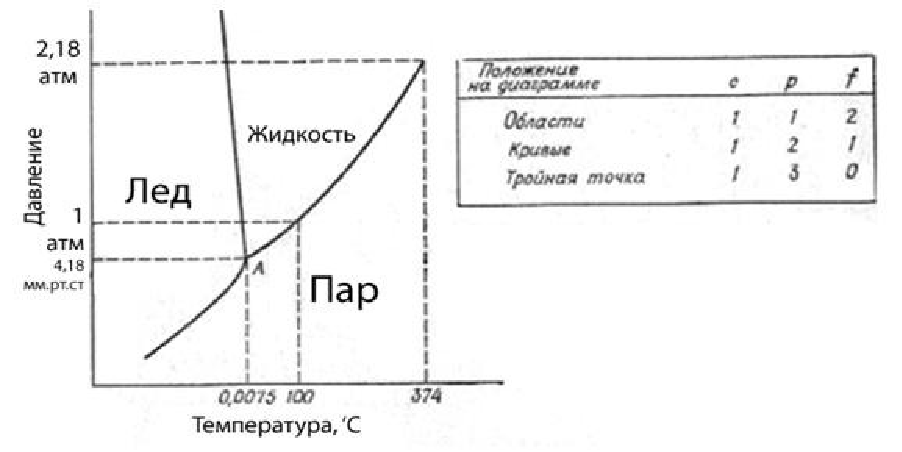
\includegraphics[width=10cm]{figures/fig_11_1.pdf}
	\caption{Схема фазовых переходов для однокомпонентной системы --- воды.}
	\label{fig.111}
\end{figure}

Согласно правилу фаз Гиббса для однокомпонентной системы ($c = 1$) в зависимости от числа фаз $p$ (1, 2 или 3) существует $f$ (2, 1 или 0) степеней свободы.

Биологические мембраны не являются статическими структурами, их внутренняя область может обладать некоторой степенью <<текучести>>, которая коррелирует с биологическими функциями (транспорт углеводов) или со степенью анестезии, вызываемой анестетиками. 

Важно, что биологические мембраны являются многокомпонентными системами. Согласно правилу фаз Гиббса, при существовании двух фаз (например, твердой и жидкой) в системе, содержащей всего два компонента ($c = 2$), система обладает двумя степенями свободы. То есть, двухкомпонентная система в общем случае не характеризуется четко выраженной температурой плавления, поскольку при изменении температуры в некоторых пределах в системе находятся две фазы.

Биологическое значение этой особенности очевидно: если бы биологические мембраны были построены из липидов только одного типа, мембрана бы обладала резкой температурой плавления, и организм мог бы отвечать на колебания температуры изменением состояния и, следовательно, функции мембраны только по типу <<все-или-ничего>>. Однако, благодаря многокомпонентному составу мембрана может претерпевать постепенные изменения степени текучести в широком интервале температур, обеспечивая гораздо более <<тонкий>> контроль за функцией клетки в соответствии с температурой окружающей среды.



Многокомпонентный мембраны необходимы клетке, чтобы реагировать на изменение температуры и формировать липидные рафты.


\newpage
%%%%%%%%%%%%%%%%%%%%%%%%%%%%%%%%%%%%%%%%%%%%%%%%%%%%%%%%%%%%%%%%%%%%%%%%%%%%%%%%%%%%%%%%
\section{Осмотическое давление}
{\it Вывод формулы для расчета осмотического давления. Значение осмотического давления для биологических систем. Определение молекулярной массы веществ по величине осмотического давления.}

\subsection{Вывод формулы для расчета осмотического давления}

\begin{figure}[ht] \center
\label{fig.131}
	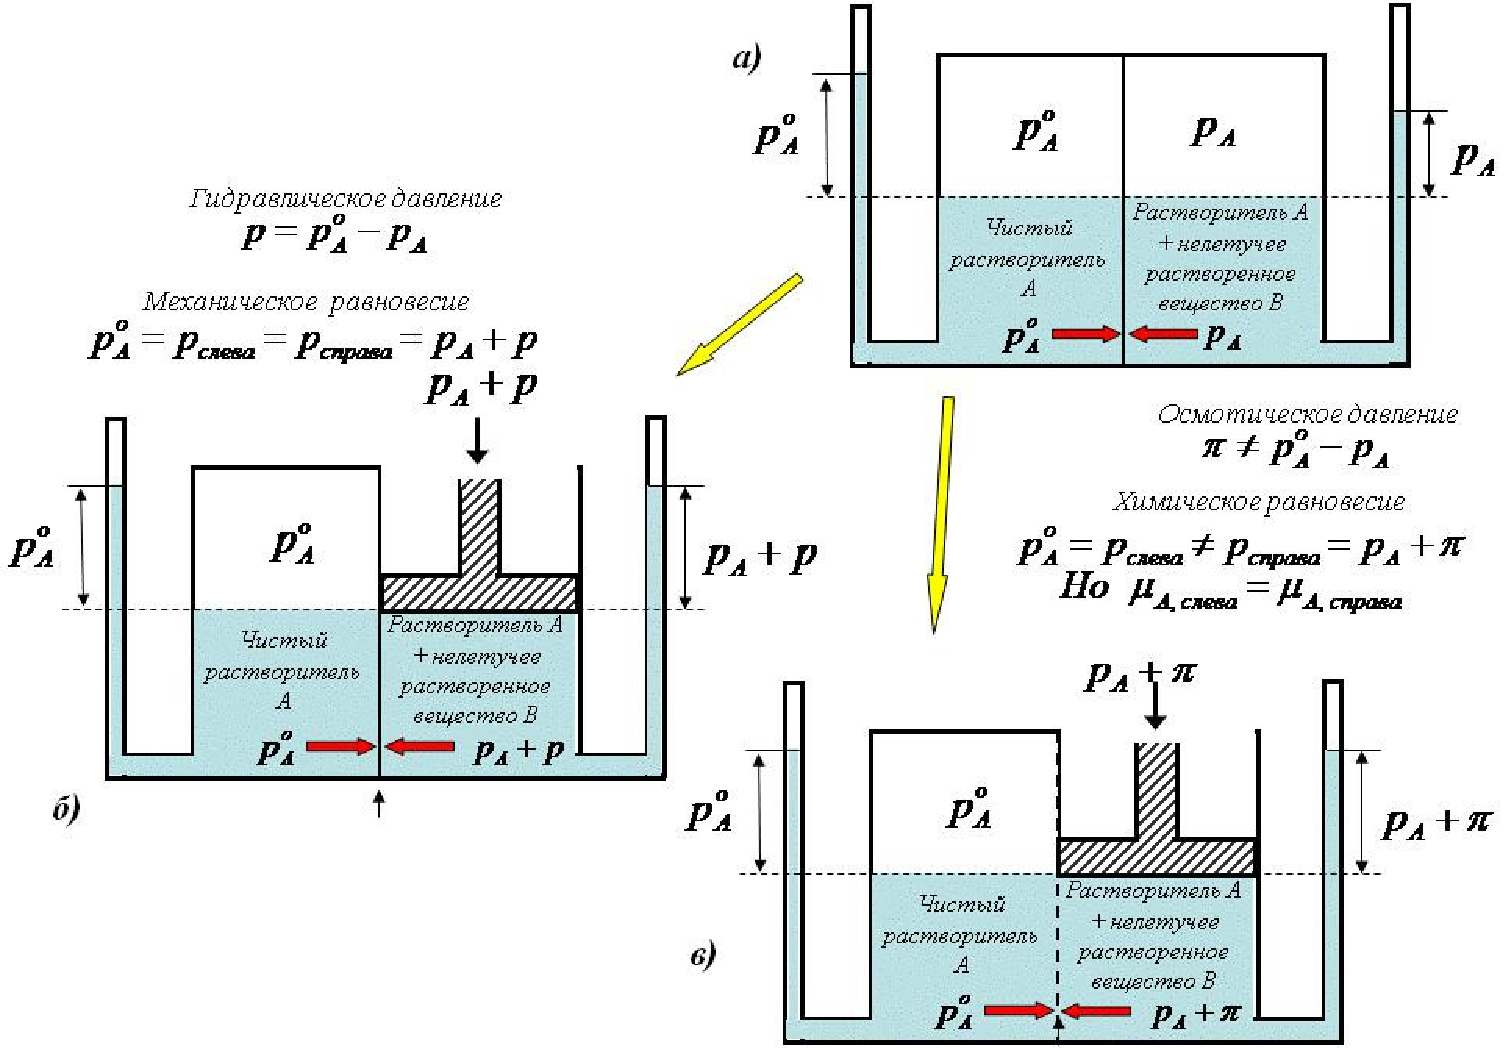
\includegraphics[width=10cm]{figures/fig_13_1.pdf}
	\caption{Уточнить точную формулировку картинки}
\end{figure}

Парциальное давление насыщенного пара компонента раствора прямо пропорционально его мольной доле в растворе, причем коэффициент пропорциональности равен давлению насыщенного пара над чистым компонентом:
\begin{equation}
	p_A = p_A^0 X_A,
\end{equation}
где $p_A$ --- давление насыщенного пара;\\
$p_A^0$ --- давлению насыщенного пара над чистым компонентом;\\
$X_A$ --- мольная доля молекул растворителя.

Связь между химическим потенциалом и давлением:
\begin{equation}
	dG=VdP-SdT+\mu_A dN_A+\mu_B dN_B
\end{equation}

\begin{equation}
	\left( \frac{\partial G}{\partial p}\right)_{T, n_A , n_B} = V	
	\qquad \Rightarrow \qquad
	\left( \frac {\partial}{\partial n_A}V \right)_{T,p,n_B} = \overline{V}_A
\end{equation}

$\overline{V}_A$ --- парциальный моляльный объем растворителя

\begin{equation}
\begin{array}{l} 
	\left(\frac {\partial}{\partial n_A}\right)\left( \frac{\partial G}{\partial p}\right)_{T, n_A , n_B}= \overline{V}_A=\\
	\left( \frac{\partial }{\partial p}\right)\left( \frac {\partial G}{\partial n_A}V \right)_{T,p,n_B} = \frac {\partial}			{\partial p} \mu _A
\end{array} 
\end{equation}

$\left(\frac{\partial \mu_A }{\partial p}\right)_{T, n_A , n_B} = \overline{V}_A$ $d \mu_A = (\overline{V}_A)_{\text {жидк.}} dp$ --- для жидкости

\begin{equation}
\begin{array}{l} 
	\mu _A = \mu _{A (\text{станд. сост.})} + \int \limits_{\text{ст. сост}}^{\text{эксп. сост}} d \mu _A = \mu _A^0 + 		\int \limits_{\text{ст. давл}}^{\text{эксп. давл}} \overline{V}_A dp
\end{array} 
\end{equation}

Для несжимаемой жидкости макроскопические изменения химического потенциала равны:

\begin{equation}
	\mu _A= \mu _A^0 + \overline{V}_A \int \limits _{p_A^0}^p dp \Rightarrow \mu _A= \mu _A^0 + \overline{V}_A (p - p_A^0)
\end{equation}

Для пара (согласно закону идеальных газов $\overline{V}_A = \frac {RT}{p_A}$)

\begin{equation}
	d\mu _A=RT \frac {dp_A} {p_A} \enskip \text {отсюда} \enskip d\mu _A=RT d\ln (P_A)
\end{equation}

\begin{equation}
	\mu _ A = \mu _A^0 + RT\int \limits_\text {станд. сост.}^\text {эксп. сост.} d \ln p
\end{equation}

\begin{equation}
\begin{array}{l} 
	\mu _ A = \mu _A^0 + RT\int \limits_\text {1 атм}^\text {p атм} d \ln p = \\
	= \mu _A^0 + RT (\ln p - \ln 1) = \mu _A^0 +RT \ln \left( \frac p 1\right)
\end{array} 
\end{equation}

$\mu _A^0 +RT \ln (p) $ --- (постоянная температура, идеальный газ, $p$ в атмосферах)

Любой раствор находится в равновесии со своим паром:

\begin{equation}
\begin{array}{l} 
	(\mu _ A)_\text {пар, слева}= (\mu _ A)_\text {жидк., слева}, \\
	(\mu _ A)_\text {пар, справа}= (\mu _ A)_\text {жидк., справа}
\end{array} 
\end{equation}

\begin{equation}
\begin{array}{l} 
	(\mu _ A)_\text {жидк., слева}-(\mu _ A)_\text {жидк., справа}= \\
	=(\mu _ A)_\text {пар, слева}-(\mu _ A)_\text {пар, справа}
\end{array} 
\end{equation}

\begin{equation}
\begin{array}{l} 
	(\mu _ A)_\text {жидк., слева}-(\mu _ A)_\text {жидк., справа}= \mu _A^0 +RT \ln p_A^0 - \\
	- (\mu _A^0 +RT \ln p_A) = RT \ln \left( \frac {p_A^0}{p_A} \right) = -RT \ln \left( \frac {p_A}{p_A^0} \right)
\end{array}
\end{equation}

\begin{equation}
	(\mu _ A)_\text {жидк., слева}-(\mu _ A)_\text {жидк., справа}= -RT \ln \left( X_A \right)_\text {справа}
\end{equation}

Важность этого уравнения в том, что поскольку $X_A$ справа < 1, то на основании этого можно сделать вывод, что химический потенциал растворителя А (слева от мембраны) больше химического потенциала раствора (справа от мембраны). Следовательно, молекулы растворителя проявляют тенденцию к миграции через полупроницаемую мембрану для уменьшения своего химического потенциала.

Химический потенциал жидкого растворителя можно увеличить, наложив внешнее давление $\pi$ к раствору, так чтобы его химический потенциал увеличился на величину точно равную начальной разности химических потенциалов растворителя и раствора:

\begin{equation}
	\begin{array}{l} 
		\bigtriangleup(\mu _A)_\text {жидк., справа} = (\overline{V}_A)_\text {жидк.}(P_A + \pi - P_A^0) - \\
		- (\overline{V}_A)_\text {жидк.}(P_A - P_A^0) = \pi (\overline{V}_A)_\text {жидк.}
	\end{array}
\end{equation}

$\pi (\overline{V}_A)_\text {жидк.} = -RT \ln \left( X_A \right)_\text {справа}$ --- осмотическое давление идеального раствора.

$X_A+X_B = 1$ $\Rightarrow$ $\pi (\overline{V}_A)_\text {жидк.} = -RT \ln \left[ 1 - (X_B)_\text {справа} \right]$ 

$X_B \ll 1 \Rightarrow$

\begin{equation}
	\pi (\overline{V}_A)_\text {жидк.} \approx RT X_B = RT \frac {n_B} {n_A+n_B} \approx RT \frac {n_B} {n_A}
\end{equation}

$\pi = mRT$, где $m$ - молярная концентрация (число молей в 1 литре)

В качестве примера: различие концентраций на ~0.1 моль/л приводит к возникновению осмотического давления ~2.5 атм.

\textbf{Значение осмотического давления для биологических систем.}

Осмотическое давление в клетках животных, растений, микроорганизмов и в биологических жидкостях зависит от концентрации веществ, растворенных в их жидких средах. Солевой состав биологических жидкостей и клеток, характерный для организмов каждого вида, поддерживается избирательной проницаемостью биологических мембран для разных солей и активным транспортом ионов. Относительное постоянство осмотического давления обеспечивается водно-солевым обменом, т. е. всасыванием, распределением, потреблением и выделением воды и солей (см. Выделение, Выделительная система, Осморегуляция). У т. н. гиперосмотических организмов внутреннее осмотическое давление больше внешнего, у гипоосмотических — меньше внешнего; у изоосмотических (пойкилоосмотических) внутреннее осмотическое давление равно внешнему. В первом случае ноны активно поглощаются организмом и задерживаются в нем, а вода поступает через биологические мембраны пассивно, в соответствии с осмотическим градиентом. Гиперосмотическая регуляция свойственна пресноводным организмам, мор. хрящевым рыбам (акулы, скаты) и всем растениям. У организмов с гипоосмотической регуляцией имеются приспособления для активного выделения солей. У костистых рыб преобладающие в океанических водах ионы $Na^+$ и $Cl-$ выделяются через жабры, у морских пресмыкающихся (змеи и черепахи) и у птиц — через особые солевые железы, расположенные в области головы. Ионы $Mg^{2+}$, , у этих организмов выделяются через почки. Осмотическое давление у гипер- и гипоосмотических организмов может создаваться как за счет ионов, преобладающих во внешней среде, так и продуктов обмена. Например, у акуловых рыб и скатов осмотическое давление на 60$\%$ создается за счет мочевины и триметиламмония; в плазме крови млекопитающих — главным образом за счет ионов $Na^+$ и $Cl^-$; в личинках насекомых — за счёт разнообразных низкомолекулярных метаболитов. У морских одноклеточных, иглокожих, головоногих моллюсков, миксин и других изоосмотических организмов, у которых осмотическое давление определяется осмотическим давлением внешней среды и равно ему, механизмы осморегуляции отсутствуют (исключая клеточные).

Диапазон средних величин осмотического давления в клетках организмов, не способных поддерживать осмотический гомеостаз, довольно широк и зависит от вида и возраста организма, типа клеток и осмотического давления окружающей среды. В оптимальных условиях осмотическое давление клеточного сока наземных органов болотных растений колеблется от 2 до 16 ат, у степных — от 8 до 40 ат. В разных клетках растения осмотическое давление может резко различаться (так, у мангровых осмотическое давление клеточного сока около 60 ат, а осмотическое давление в сосудах ксилемы не превышает 1—2 ат). У гомоосмотических организмов, т. е. способных поддерживать относительное постоянство осмотического давления, средней величины и диапазон колебаний осмотического давления различны (дождевой червь — 3,6—4,8 ат, пресноводные рыбы — 6,0—6,6, океанические костистые рыбы — 7,8—8,5, акуловые — 22,3—23,2, млекопитающие — 6,6—8,0 ат). У млекопитающих осмотическое давление большинства биологических жидкостей равно осмотическому давлению крови (исключение составляют жидкости, выделяемые некоторыми железами, — слюна, пот, моча и др.). Осмотическое давление, создаваемое в клетках животных высокомолекулярными соединениями (белки, полисахариды и др.), незначительно, но играет важную роль в обмене веществ (см. Онкотическое давление).

\textbf{Определение молекулярной массы веществ по величине осмотического давления.}

Пример: в 1 мл воды растворено 80 мг исследуемого белка. Осмотическое давление этого раствора при $25^\circ C$ оказалось равным 12 мм.рт.ст. .Какова молекулярная масса исследуемого белка? 

\begin{equation}
	M = \frac {c} {\pi} RT
\end{equation}

\begin{equation}
	M (\text {г/моль}) = (80 \text{г/л})\cdot(0,08206 (\text {л атм/(моль К)})) \cdot 298K \cdot (760/12 (\text {1/атм}))
\end{equation}

Решение приводит к молекулярной массе белка равной $M = 124000$ г/моль.




\newpage
%%%%%%%%%%%%%%%%%%%%%%%%%%%%%%%%%%%%%%%%%%%%%%%%%%%%%%%%%%%%%%%%%%%%%%%%%%%%%%%%%%%%%%%%
\section{Химические реакции и константы равновесия}
{\it Активность как термодинамическая концентрация. Вывод уравнения Гиббса-Дюгема. Самопроизвольное протекание химических реакций. Вывод критерия самопроизвольности химических реакций}

\subsection{Активность как термодинамическая концентрация}



\subsection{Вывод уравнения Гиббса-Дюгема}



\subsection{Самопроизвольное протекание химических реакций}



\subsection{Вывод критерия самопроизвольности химических реакций}

Можно подобрать такие условия, что любая реакция сможет протекать самопроизвольно.




\newpage
%%%%%%%%%%%%%%%%%%%%%%%%%%%%%%%%%%%%%%%%%%%%%%%%%%%%%%%%%%%%%%%%%%%%%%%%%%%%%%%%%%%%%%%%
\section{Стационарная ферментативная кинетика}
{\it Кинетическая схема Михаэлиса-Ментен и условие стационарности. Вывод уравнения Михаэлиса-Ментен. Линеаризация уравнения Михаэлиса-Ментен по Лайнуиверу-Берку.}

Ферментативная кинетика --- раздел химической кинетики, науки о скоростях химических реакций. Механизмы этих реакций характеризуются кинетическими параметрами, к которым относится скорость химических реакций (количество вещества, прореагировавшего в единицу времени).

\subsection{Кинетическая схема Михаэлиса-Ментен и условие стационарности}

Схема Миха\'{э}лиса-М\'{е}нтен предложена в 1913 году для фермента инвертазы. Она состоит из стадий: образования фермент-субстратного комплекса $ES$, превращения субстрата $S$ в продукт $P$, наконец, десорбции продукта с фермента и восстановление последнего в первоначальное состояние $E$.

Для этой простейшей схемы ферментативного процесса с участием одного промежуточного соединения кинетику реакции
\begin{equation}
	E + S \xrightleftharpoons[~k_{-1}~]{k_1} ES \xrightarrow{~k_2~} E + P
	\label{MichaelisScheme}
\end{equation}
описывает система уравнений, включающая два дифференциальных уравнения (\ref{mm:4}, \ref{mm:3}) и уравнения материального баланса \cite{Varfolomeev2005, Beresin1979}:
\begin{align}
d{[P]} /dt & = k_2 [ES], \label{mm:4}\\
d{[ES]}/dt & = k_1 [E][S] - (k_{-1} + k_2) [ES], \label{mm:3}\\
[E]_0      & = [E] + [ES], \label{mm:2}\\
[S]_0      & = [S] + [P] + [ES]. \label{mm:1}
\end{align}

Принцип стационарности в применении к этой реакции означает, что после некоторого определенного промежутка времени с начала реакции концентрация промежуточного продукта достигает максимального значения и в течении некоторого промежутка времени практически не изменяется $[ES] = const$ \cite{Beresin1979}.

Поскольку константа скорости $k_2$ превращения фермент-субстратного комплекса $ES$ в фермент $E$ и продукт $P$ много больше (??), чем константа скорости $k_1$ образования фермент-субстратного комплекса, скорость реакции определяется распадом комплекса $ES$ (константой $k_2$) и мы считаем процесс квазистационарным ($d[ES]/dt \approx 0$). Скорость образования фермент-субстратного комплекса $ES$ равна скорости его распада. Стационарность возможна, только если субстрата много больше чем фермента $S >> E_0$.

\subsection{Вывод уравнения Михаэлиса-Ментен}

Уравнение Миха\'{э}лиса-М\'{е}нтен (\ref{MichaelisMenten}) является основным уравнением ферментативной кинетики и описывает зависимость скорости образования продукта от концентрации субстрата и фермента согласно реакции (\ref{MichaelisScheme}).

Используя условие $d[ES]/dt=0$, из уравнения (\ref{mm:3}) получим:
\begin{equation}
	\label{mm:7}
	[E] = \frac{(k_{-1} + k_2) [ES]}{k_1 [S]}.
\end{equation}

Подставим полученное выражение (\ref{mm:7}) в уравнение (\ref{mm:2}):
\begin{equation}
	\label{mm:8}
	[E]_0 = \frac{(k_{-1} + k_2) [ES]}{k_1 [S]} + [ES] = \frac{(k_{-1} + k_2) + k_1 [S]}{k_1 [S]}[ES]
\end{equation}

Из уравнения (\ref{mm:7}) выразим $[ES]$:
\begin{equation}
	\label{mm:9}
	[ES] = \frac{k_1 [S] [E]_0}{(k_{-1} + k_2) + k_1 [S]} = \frac{[S] [E]_0}{(k_{-1} + k_2)/k_1 + [S]}
\end{equation}

Найдем скорость реакции, подставим (\ref{mm:9}) в (\ref{mm:4}):
\begin{equation}
	\label{MichaelisMenten}
	v = \frac{k_2 [E]_0 [S]}{[S] + (k_2 + k_{-1})/k_1}	
	\qquad \text{или} \qquad
	\boxed{v = \frac{V_{max} [S]}{[S] + K_M}}
\end{equation}
где $K_M = (k_2 + k_{-1})/k_1$ --- константа Михаэлиса-Ментен;\\
$V_{max}$--- максимальная скорость реакции, равная $k_2 [E]_0$;\\
$[S]$ --- концентрация субстрата;\\
$[E]_0$ --- начальная концентрация фермента.\\

Для начальной стадии реакции можно пренебречь уменьшением концентрации субстрата. Тогда выражение (\ref{MichaelisMenten}) для начальной скорости реакции будет выглядеть так:
\begin{equation}
	v_0 = \frac{V_{max} [S]_0}{[S]_0 + K_M}
\end{equation}

Константа Михаэлиса характеризует сродство фермента к субстрату: высокое сродство характеризуется низкой величиной константы, и наоборот. Константа Михаэлиса численно равна той концентрации субстрата $[S]$, при которой скорость реакции достигает половины максимальной величины (Рис. \ref{mmenten}, а).

Модель Михаэлиса-Ментен основывается на нескольких нереальных допущениях:
\begin{itemize}
	\item необратимое превращение $ES$ в $E$ + $P$;
	\item достижение равновесия между $E$, $S$ и $ES$;
	\item отсутствие в растворе других форм фермента, кроме $E$ и $ES$.
\end{itemize}

\begin{figure}[ht] \center
	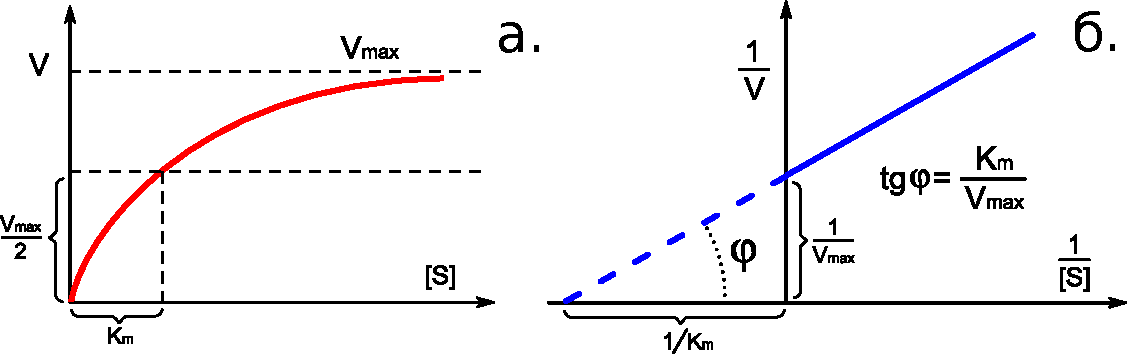
\includegraphics[width=10.5cm]{figures/menten.pdf}
	\caption{\textbf{a.} Зависимость скорости реакции от концентрации субстрата. \textbf{б.} Линеаризованная форма зависимости в обратных координатах (по Лайнуиверу-Берку)}
	\label{mmenten}
\end{figure}


\subsection{Линеаризация уравнения Михаэлиса-Ментен по Лайнуиверу-Берку}

Для удобства расчетов уравнение (\ref{MichaelisMenten}) возможно преобразовать так, чтобы экспериментальные точки лежали на прямой. Для простого графического определения констант часто используют различные линеаризации уравнения. Наиболее часто используется линеаризация Лайнуивера-Берка.

Перевернем уравнение (\ref{MichaelisMenten}) и получим:
\begin{equation}
	\label{linearMM}
	\frac 1 V = \frac{[S] + K_M}{V_{max} [S]}, \quad
	\rightarrow \quad \frac 1 V = \frac{K_M}{V_{max} [S]} + \frac{[S]}{V_{max} [S]},
\end{equation}
линейную зависимость от обратных координат (см. Рис. \ref{mmenten}, б):
\begin{equation}
	\label{lainuiverBerk}
	\frac 1 V = \frac{K_M}{V_{max}} \frac{1}{[S]} + \frac{1}{V_{max}}.
\end{equation}

Уравнение (\ref{lainuiverBerk}) является уравнением Лайнуивера-Берка.




\newpage
%%%%%%%%%%%%%%%%%%%%%%%%%%%%%%%%%%%%%%%%%%%%%%%%%%%%%%%%%%%%%%%%%%%%%%%%%%%%%%%%%%%%%%%%
\section{Нестационарная ферментативная кинетика}
{\it Релаксационные методы исследования ферментативных реакций. Основные экспериментальные способы измерения характеристик нестационарных ферментативных процессов.}

\subsection{Релаксационные методы исследования ферментативных реакций}
% Волькенштейн М.В. Биофизика. Москва: Наука, 1988. С. 592., стр. 205.

Нестационарная ферментативная кинетика и, тем самым, механизм действия ферментов эффективно изучаются методами химической релаксации, развитыми Эйгеном. Система выводится из равновесного или стационарного состояния быстрым изменением внешнего параметра и изучается кинетика ее приближения к новому равновесному или стационарному состоянию. Чаще всего пользуются скачком концентрации или температуры, воздействием ультразвука и др. Доступны измерению времена релаксации вплоть до $10^{-10}$с \cite{Volkenshtejn1988}.

Рассмотрим простейшую одностадийную реакцию:
\begin{equation}
	\label{sligand:1}
	F_0 + S \xrightleftharpoons[~k_{-1}~]{k_1} F_1
\end{equation}
где $S$ --- лиганд.\\

Кинетическое уравнение имеет вид:
\begin{equation}
	\label{sligand:2}
	\dot{F_0} = - k_1 F_0 S + k_{-1} F_1
\end{equation}

В стационарном состоянии: $\dot{F_0} = \dot{F_1} = \dot{S} = 0$. Выведем систему из равновесия небольшим возмущением какой-либо переменной:
\begin{equation}
	\label{sligand:4}
	F_0 = \overline{F_0} + x_0, \qquad F_1 = \overline{F_1} + x_1, \qquad S = \overline{S} + y,
\end{equation}
где $\overline{F_0}, \overline{F_1}, \overline{M}$ --- стационарные концентрации;\\
$x_0, x_1, y$ --- отклонения концентраций при возмущении.

Тогда, подставив (\ref{sligand:4}) в (\ref{sligand:2}), динамика возмущения:
\begin{equation}
	\label{sligand:5}
	\dot{x_0} = - k_1 \overline{F_0} y - k_1 \overline{S} x_0 - k_1 x_0 y + k_{-1} x_1.
\end{equation}

Из закона сохранения для реакции (\ref{sligand:1}):
\begin{equation}
	\label{sligand:6}
	x_0 = y = - x_1.
\end{equation}

В уравнении (\ref{sligand:5}) пренебрегаем $k_1 x_0 y = 0$, в силу того, что в нем два малых возмущения. Тогда с учетом (\ref{sligand:6}) получим:
\begin{equation}
	\label{sligand:7}
	\dot y = - (k_1 \overline{F_0} - k_1 \overline{S} + k_{-1} ) y.
\end{equation}

Тогда после разнесения переменных в (\ref{sligand:7}) получим:
\begin{equation}
	\label{sligand:8}
	\frac{dy}{y} = - (k_1 \overline{F_0} - k_1 \overline{S} + k_{-1} ) dt,
\end{equation}

и решение этого уравнения (\ref{sligand:8}) будет:
\begin{equation}
	\label{sligand:9}
	y(t) = y(0) \exp (-t / \tau ),
\end{equation}
где $\tau = k_1 (\overline{F_0} \, \overline{S}) + k_{-1}$.

Измерение $\tau$ при разных концентрациях $\overline{F_0}$ и $\overline{S}$ позволяет определить $k_1$ и $k_{-1}$.



\subsection{Основные экспериментальные способы измерения характеристик нестационарных ферментативных процессов}

Кинетика ферментативных реакций в предстационарном режиме их протекания изучается в основном <<струевыми>> методами, которые позволяют смешать два раствора за доли миллисекунды, в то время как число оборотов большинства ферментов составляет около $1000 c^{-1}$, и методами релаксационной кинетики. Проблема мертвого времени, связанного со смешиванием реагентов, здесь отсутствует, благодаря использованию предварительно смешанных растворов. 

<<Струевые>> методы для измерения кинетики быстрых реакций в растворе впервые были использованы Хартриджем и Роутоном в 1923 г. Сущность <<струевых>> методов заключается в том, что реакция инициируется быстрым смешиванием реагентов в проточных условиях. Различают 3 <<струевых>> метода: метод непрерывной струи, ускоренной и остановленной струи. По методу непрерывной струи два раствора реагирующих веществ вводят в смесительную камеру, и раствор после смешивания поступает в трубку для наблюдения.

\begin{figure}[ht] \center
	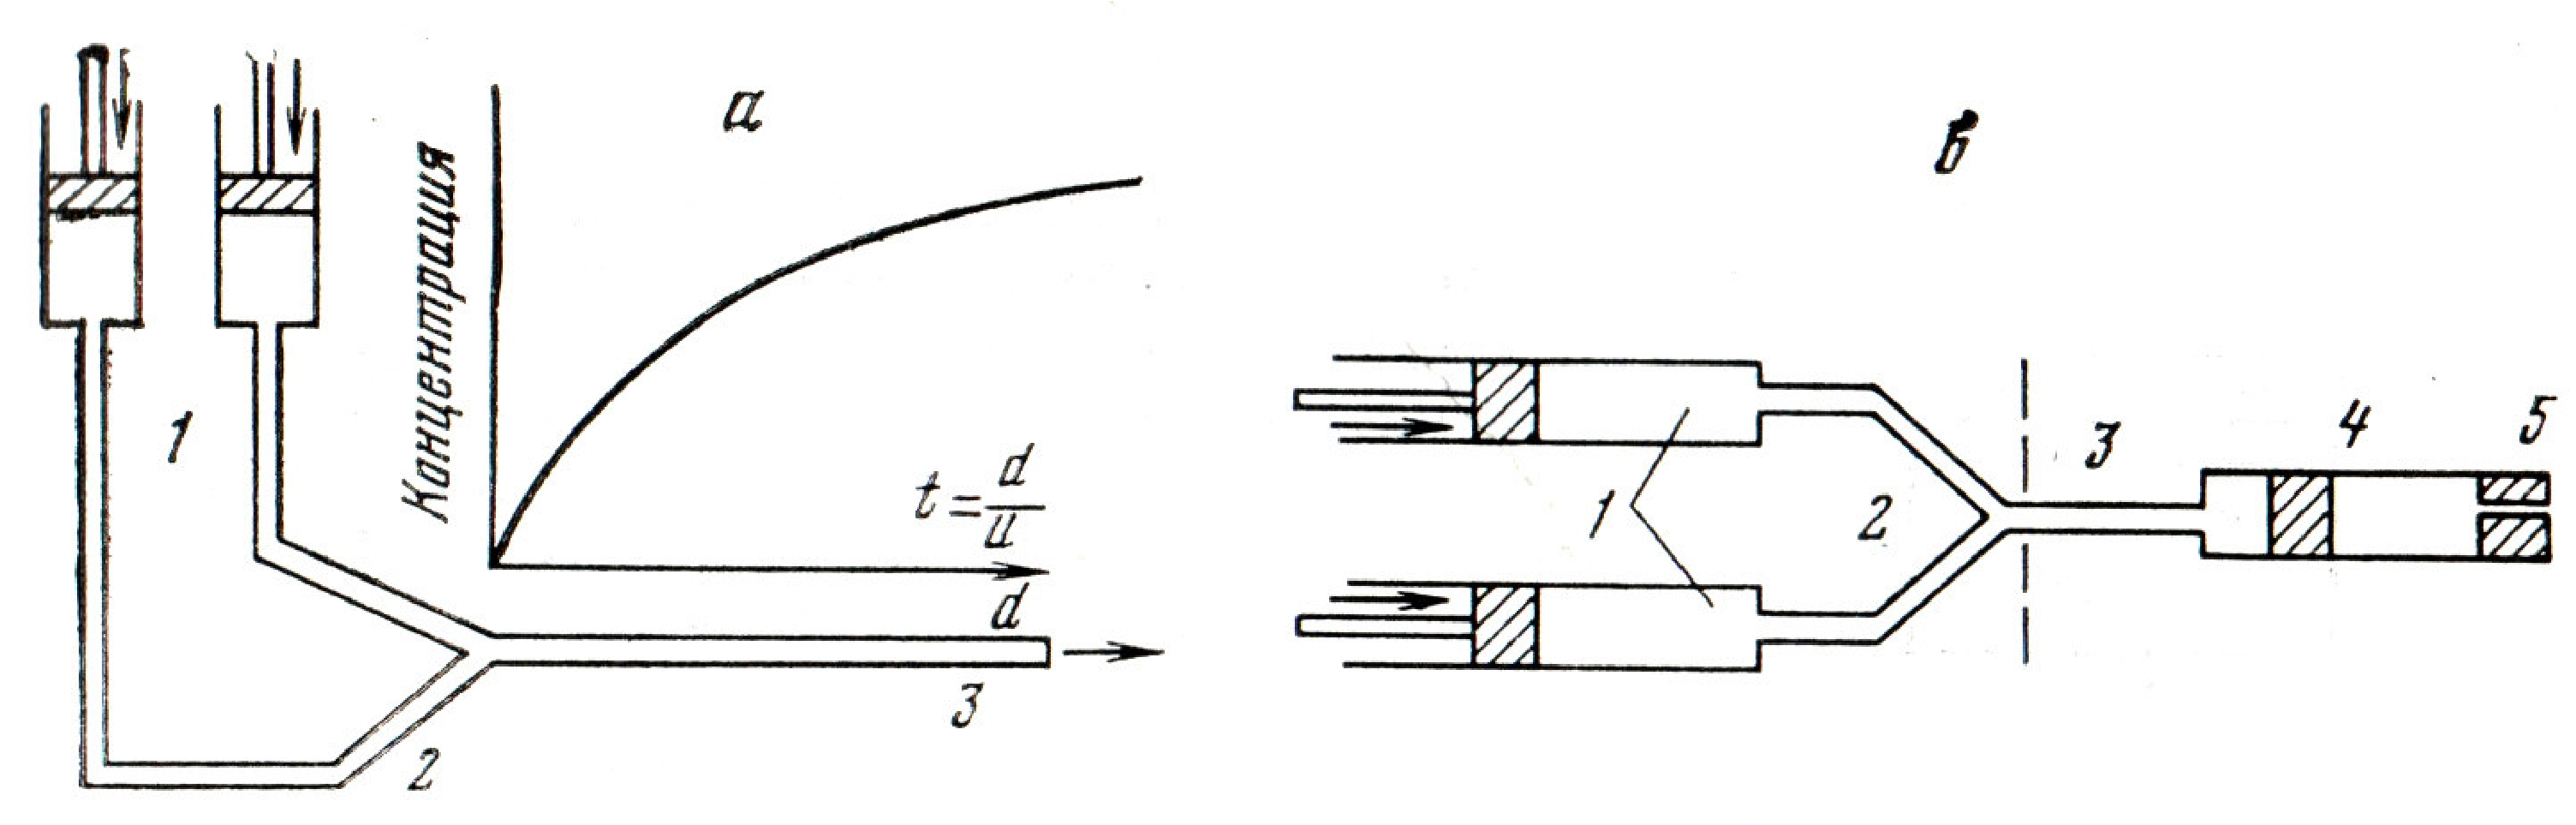
\includegraphics[width=10.5cm]{figures/sf1.pdf}
	\caption{\textbf{a.} Принципиальная схема установки, используемой в методе непрерывной струи: 1 --- растворы реагирующих веществ; 2 --- смесительная камера; 3 --- трубка для наблюдений \textbf{б.}  Принципиальная схема установки, используемой в методе остановленной струи: 1 --- растворы реагирующих веществ; 2 --- смесительная камера; 3 --- точка наблюдения; 4 --- останавливающий поршень; 5 - ограничитель \cite{Beresin1979}}
	\label{sf1}
\end{figure}


Время $t$ в этом методе при постоянной скорости потока $u$ определяется расстоянием $l$ от смесительной камеры: $t = l/u$. Например, если скорость струи равна 10 м/с, то на расстоянии 1 см от смесителя <<возраст>> раствора будет равен 1 мс, на расстоянии 10 см -- 10 мс и т. д. 

По методу ускоренной струи растворы реагирующих веществ помещают в шприцы, поршни которых приводят в движение резким толчком в течение примерно 0,1 с. Наблюдение проводят в фиксированной точке вблизи смесительной камеры. При этом скорость течения жидкости (и, следовательно, время протекания реакции) постоянно меняется. Методика ускоренной струи позволяет использовать весьма малые объемы реагирующих веществ (до 0,1 мл), что является важным преимуществом при исследовании ферментативных реакций.

Наиболее широкое распространение нашел метод остановленной струи. 

Для остановки струи используют простое устройство, которое позволяет остановить поток за 1-2 мс. Это устройство представляет собой поршень, помещенный в конце трубки для наблюдений. Реакционная смесь толкает этот поршень, и он резко останавливается, дойдя до внешних ограничителей.

Чаще всего в <<струевых>> методах используют спектрофотометрический метод измерения с осциллографической регистрацией сигнала от фотоумножителя. <<Мертвое>> время лучших современных установок подобного типа составляет 0,1 - 0,3 мсек. Следовательно, <<струевые>> методы не позволяют изучать нестационарную кинетику в микросекундном режиме.


\textbf{Метод импульсного фотолиза (флеш-метод)}

Дальнейшее увеличение временной разрешающей способности аппаратуры для исследования нестационарной кинетики дает использование в энзимологии метода импульсного фотолиза. Этот метод применяется для реакций, которые инициируются действием света за счет протекающих в системе фотохимических реакций. В отличие от "струевых" методов метод импульсного фотолиза не требует быстрого смешивания реагентов. 
\begin{figure}[ht] \center
	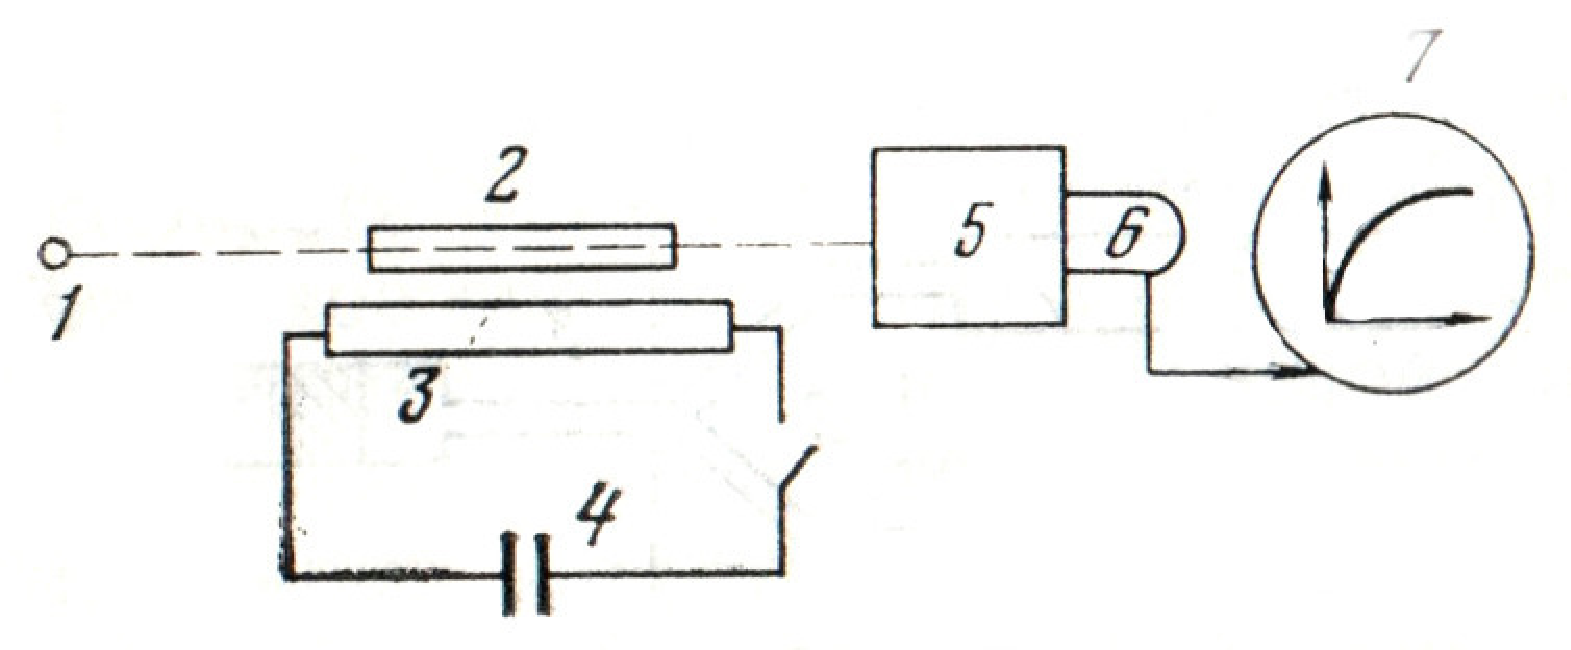
\includegraphics[width=7cm]{figures/sf2.pdf}
	\caption{Принципиальная схема установки импульсного фотолиза: 1 --- источник света; 2 --- кювета с исследуемым раствором; 3 --- импульсная лампа; 4 --- высоковольтный конденсатор; 5 - монохроматор; 6 --- фотоумножитель; 7 --- осциллограф  \cite{Beresin1979}}
	\label{sf2}
\end{figure}

Реакция инициируется под действием мощного светового импульса на раствор фермента с веществом, которое под действием света превращается в субстрат (или эффектор ферментативного процесса). Фотохимическая реакция может протекать и в активном центре фермента. Продуктом такой реакции является активный фермент, который начинает катализировать исследуемую реакцию.

<<Мертвое>> время метода определяется двумя параметрами: 1) временем импульсной вспышки и 2) временем фотохимического образования соответствующего компонента ферментативной реакции. Ксеноновая импульсная техника позволяет получить мощные импульсы света продолжительностью 10--100 мксек. Время вспышки может быть уменьшено без уменьшения мощности при использовании лазерной техники. Время фотохимической реакции может быть достаточно коротким.





\newpage
%%%%%%%%%%%%%%%%%%%%%%%%%%%%%%%%%%%%%%%%%%%%%%%%%%%%%%%%%%%%%%%%%%%%%%%%%%%%%%%%%%%%%%%%
\section{Теория переходного состояния и скорости химических реакций}
{\it Температурная зависимость индивидуальных констант скоростей реакции. Теория переходного состояния и скорости химических реакций. Денатурация белков. Термодинамические характеристики ферментативной реакции.}

\subsection{Температурная зависимость индивидуальных констант скоростей реакции}





\chapter{Молекулярная биология клетки}

%%%%%%%%%%%%%%%%%%%%%%%%%%%%%%%%%%%%%%%%%%%%%%%%%%%%%%%%%%%%%%%%%%%%%%%%%%%%%%%%%%%%%%%%
\section{Биологические молекулы и их окружение}
{\it Основные меж- и внутримолекулярные силы, обеспечивающие формирование и поддержание структуры биомолекул и их комплексов. Пространственная организация биополимеров. Электронные свойства биополимеров.}

\subsection{Основные меж- и внутримолекулярные силы, обеспечивающие формирование и поддержание структуры биомолекул и их комплексов}


Волькенштейн, Рубин.



\newpage
%%%%%%%%%%%%%%%%%%%%%%%%%%%%%%%%%%%%%%%%%%%%%%%%%%%%%%%%%%%%%%%%%%%%%%%%%%%%%%%%%%%%%%%%
\section{Структура и функция белков}
{\it Классификация структур белков. Принципы структурной организации белков. Переходы спираль-клубок. Кооперативные переходы в белковых молекулах. Формирование пространственной организации белков. Проблема предсказания пространственной структуры белков по первичной структуре.}

\subsection{Классификация структур белков}

Структура функция --- много к одному.

Белки можно разбить на два больших класса: глобулярные белки и фибриллярные белки.

\textbf{Глобулярные}: белки, у которых одна или большее число полипептидных цепей свернуты в
плотную компактную структуру сферической (или глобулярной) формы. Обычно глобулярные белки
растворимы в водных системах и легко диффундируют; одни из этих белков выполняют функции,
обусловленные их подвижностью, а другие функционируют как динамические системы. К глобуляр-
ным белкам относятся почти все ферменты, равно как и транспортные белки крови, антитела и пище-
вые белки.

\textbf{Фибриллярные}: белки, молекулы которых представляют собой нерастворимые в воде длинные
нитевидные полипептидные цепи, вытянутые вдоль одной оси. Типичными фибриллярными белками
являются альфа-кератин волос и шерсти, фиброин шелка и коллаген сухожилий. К этому классу от-
носятся также нитевидные белки, присутствующие в сократительных системах мышечных и немы-
шечных клеток, например, актин и миозин, а также микротрубочки.

\textbf{Мембранные белки}.

\textbf{Короткие пептиды}.



\subsection{Принципы структурной организации белков}

Существует два информационных уровня организации белковых (и других) макромолекул.

Первый уровень --- осуществляется последовательное ковалентное соединение соответствующих
аминокислот в длинные полипептидные цепи.

Аминокислотный код является тем молекулярным кодом, с помощью которого осуществляется
сначала преобразование, а затем, и, через деятельность белков, --- воплощение и реализация генетической информации.

Подробное изучение глобулярных и фибриллярных белков показало, что для каждого индивидуального белка характерна своя пространственная трехмерная организация, которая зависит от его
первичной структуры --- то есть от информации, записанной линейным аминокислотным кодом. Генетическим кодом кодируется только первичная --- “линейная” структура полипептидной цепи. Вторичная, третичная и четвертичная структуры белковых макромолекул кодируются и программируются уже другим молекулярным кодом --- аминокислотным кодом. Первый уровень организации белковых молекул характеризуется применением линейного аминокислотного кода, который служит основой преобразования линейной формы информации полипептидов в стереохимическую форму информации белковых молекул.

Второй уровень организации белковых молекул --- пространственный, осуществляется уже при помощи химических связей, значительно более слабых, чем ковалентные. К таким связям относятся слабые: водородные и ионные связи, ван-дер-ваальсовы силы, гидрофобные взаимодействия, которые в совокупности оказываются весьма сильными. Через посредство этих сил и связей идёт воплощение линейной молекулярной информации в пространственную структуру и стереохимическую форму информации белковых молекул. В результате всех преобразований «одномерная» молекулярная информация полипептидных цепей «сворачивается, пакуется и сжимается» в трёхмерную информацию белковых молекул, которая в таком виде становится пригодной для транспортировки, передачи по различным каналам и компартментам, а затем, и для непосредственного использования в различных биологических процессах.

Наличие в структурах белковых макромолекул как внутримолекулярных, так и внешних информационных сил и связей взаимодействия позволяет говорить о том, что внутри и вокруг макромолекулы образуется специфическое силовое «информационное поле», способное влиять как на структуру самого белка, так и на его микроокружение. Поэтому белковая макромолекула как бы стабилизируется самосогласованным сжимающим информационным полем, обусловленным кооперативными силами притяжения между боковыми атомными R-группами аминокислот.

Белок не обладает сильной структурной жесткостью, он подвижен в пределах, необходимых для выполнения ими биологических функций.

Первичная структура --- последовательность аминокислот.
Вторичная (2D) --- $\alpha$-спирали, $\beta$-структуры.
Третичная (3D) (домены) --- укладка вторичных структур одной полипептидной цепи в глобулу.
Четвертичная --- объединение нескольких белковых цепей с «суперглобулу».


\subsection{Переходы спираль-клубок}

Эта теория должна давать выражения для зависимости числа разорванных водородных связей от температуры. В $\alpha$-спирали каждое звено соединено водородными связями с двумя другими, отстоящими от него на четыре звена в цепи. Для освобождения данного звена надо одновременно разорвать не две, а сразу несколько водородных связей. Теория переходов спираль-клубок основана на одномерной модели кооперативных явлений. Энергия всей цепи зависит от набора свободных и связанных звеньев, поскольку их энергии отличаются друг от друга. Для нахождения условий перехода спираль-клубок необходимо вычислить статистическую сумму цепи, учитывая всевозможные распределения водородных связей между звеньями.

Статистическая сумма цепи равна:
\begin{equation}
	Z = \sum_{\mu_i} exp ( -G {\mu_i} / RT ),
\end{equation}
где $G$ --- собственная энергия $i$-го звена, включающая и энергию его водородных связей ($G=0$ для
звена в свободном состоянии, $G=1$ --- в связанном состоянии).

В произведении $Z$ наибольшее значение имеют два типа множителей, которые определяют энергию состояния звена, следующего за связанным или за свободным звеньями. Множитель для каждого звена в связанном состоянии ($\mu_i=1$) равен
\begin{equation}
	S = \exp( - \Delta G/RT ) = exp [ - ( \Delta H - T \Delta S )/RT ] ,
\end{equation}
где $\Delta H$ определяет суммарное изменение энергии связей при фиксации звена, a $\Delta S$ включает уменьшение энтропии при ограничении его подвижности. $S$ определяет долю спирализованных
звеньев в цепи.

Другой множитель в Z для каждого звена в связанном состоянии ($\mu_i=1$), следующего за тремя (и более) свободными звеньями ($\mu_{i-1}=\mu_{i-2}=\mu_{i-3}=0$), равен $\sigma = exp( -G_{inic} RT)$, где $G_{inic}$ --- энергия инициирования спирального участка. Эта энергия затрачивается для закрепления сразу четырех звеньев, что необходимо для фиксации одного звена, следующего за тремя свободными. Фактически в этом случае при фиксации одного звена организуется сразу целый спиральный участок с понижением энтропии, что и является следствием кооперативности системы.

Степень кооперативности процесса тем больше, чем меньше множитель, зависящий от понижения энтропии при фиксации одного звена.

При $\sigma = 1$ кооперативность отсутствует ($G_{inic} = 0$),
$Z = (1 + S^N)$, где $N$ --- число звеньев в цепи.

$ \alpha= 0$ (полная кооперативность, $G_{inic} \rightarrow $)
При
$$Z = 1+ S^N$$.

В этом случае цепь находиться только в двух состояниях:
полная спиральность ($S>1$) и клубок ($S<1$);
• при $S > 1$, $S^N>>1$ --- цепь является полностью спиралью,
• при $S<1$, $S^N<<1$, $Z_\text{клуб}=1$ --- цепь переходит в состояние клубка.
• при $S = 1$ --- происходит резкий кооперативный переход спираль-клубок. Этот результат следует и из условия $\alpha = exp(-G_{inic} RT )$, так как при бесконечно большой энергии инициирования спирального участка в цепи невозможно сосуществование в одной молекуле спиральных и клубкообразных областей. В реальных системах имеется некоторый небольшой, но конечный интервал изменения температуры, ширина которого определяет область сосуществования спиральных и клубкообразных участков цепи.

\subsection{Кооперативные переходы в белковых молекулах}

Сила взаимодействия атомов или молекул возрастает по мере нарастания изменений в системе, делая их коллективно согласованными. Кооперативность нельзя объяснить простым сложением свойств отдельных атомов и молекул, ее природа --- в кооперации элементов системы, в результате которой система ведет себя как единый ансамбль, подчиняющийся определенному закону изменения. Когда субстрат связывается с активным сайтом одной субъединицы фермента, остальные субъединицы активируются.

Изменение энергии молекулы при образовании водородной связи одним из звеньев существенно зависит от наличия или отсутствия водородных связей у соседних с ним звеньев. Эта кооперативность носит энтропийный характер.

Если разность энергий состояний спираль-клубок $\Delta G = \Delta H - T \Delta S$ , $S$ известна как функция температуры, то доля спирализованных звеньев $\Theta$ может быть найдена по формуле:
\begin{equation}
	\Theta = \frac{\exp(\Delta G/RT)}{1 + \exp(\Delta G/RT)},
\end{equation}
а соответственно доля расплавленного материала составит
\begin{equation}
	1 - \Theta = \frac{1}{1 + \exp(\Delta G/RT)},
\end{equation}

Резкость перехода при нагревании можно вычислить, дифференцируя выражение по $T$ и учитывая, что при $T = T_\text{пл}$, $\Delta G = 0$, $ |\frac{d \Theta}{dT}|_{T_\text{пл}} = |\frac{\Delta H}{4RT^4}|$, где $H$ --- энтальпия перехода спираль --- клубок. Величина $\Delta H$ должна зависеть от числа $n$ освобожденных звеньев, т.е. $\Delta H \approx n \Delta H_0$ , где $H_0$  --- энтальпия разрыва связей одного звена. Кооперативный характер процесса плавления означает, что в области перехода одновременно меняется состояние n звеньев цепи, а резкость перехода пропорциональна $n$.

Формирование пространственной организации белков Первым белком, пространственная структура которого была установлена на основе анализа картины диффракции рентгеновских лучей на кристалле этого белка, был фибриллярный белок фиброин шелка. Первыми глобулярными белками, элементы пространственной структуры которых были определены с помощью рентгено-структурного анализа их кристаллов, были эдестин, альбумин и эксельстин.


\subsection{Формирование пространственной организации белков}

Общие черты пространственных структур белков:
1. Длины связей и величины валентных углов всех пептидых груп - одинаковы.
2. Все атомы пептидной группы расположены в одной плоскости и предпочтительной конфи-
гурацией пептидной группы является транс-конфигурация.
3. Полипептидная цепь полностью насыщена водородными связями.
4. Двухгранные углы вращения вокруг связей N - Cа и Cа - С' отвечают минимумам торсион-
ных потенциалов, а расстояния между всеми валентно не связанными атомами превышают суммы
ван-дер-ваальсовых радиусов.
5. Конформационные состояния всех звеньев полипептидной цепи эквивалентны.

Была сформулирована гипотеза, согласно которой $\alpha$-спираль и складчатая $\beta$-структура имеют
фундаментальное значение в пространственной организации белковых молекул и что структуры
фибриллярных, глобулярных белков и синтетических пептидов могут быть описаны с помощью не-
большого числа канонических форм --- некоторых структурных блоков.
Общая структура свернутого белка исключительно компактна. По плотности упаковки белки
очень близки кристаллам малых органических молекул (70-78 %) , связанных между собой дисперси-
онными силами. Из-за высокой плотности упаковки белки отличаются слабой сжимаемостью. Так их
коэффициент сжимаемости меньше, чем у масла, и практически совпадает с коэффициентами сжи-
маемости олова и каменной соли.
Проблема предсказания пространственной структуры белков по первичной структуре

Стратегии предсказания белковых структур:
1. Структура ищется как результат кинетического процесса сворачивания (существенного прогресса нет, т.к. сложные расчеты и весьма приблизительные потенциалы взаимодействия).
2. Ищется структура с минимальной возможной для данной цепи свободной энергией.

Оценка стабильности различных структур базируется на потенциалах взаимодействий, либо на частотах встречаемости разных структурных элементов и разных взаимодействий в белках. Здесь нет принципиальной разницы: квази-Больцмановская статистика белковых структур определяется потенциалами взаимодействий (при взаимодействии с водой используются гидрофобные взаимодействия).

Мы можем предсказать вторичную структуру белка по ее аминокислотной последовательности до предсказания третичной структуры, но не абсолютно точно. Все закономерности, наблюдающиеся в структурах белков, носят вероятностный, частотный характер. Невозможно выделить четкого кода белковых структур. Мы пытаемся предсказать вторичную структуру белка только по части тех взаимодействий, что ее держат в действительности (знаем внутренние взаимодействия, но не знаем те, что действуют между куском цепи и остальной глобулой). Точность распознавания $\alpha$- и $\beta$-структуры и нерегулярных петель белка по одной его аминокислотной последовательности 65%.


\textbf{Парадокс Левинталя} --- в 1968 году Сайрус Левинталь сформулировал известный парадокс: <<Промежуток времени, за который полипептид приходит к своему скрученному состоянию, на много порядков меньше, чем если бы полипептид просто перебирал все возможные конфигурации>>

Чтобы разрешить данный парадокс, необходимо ответить на вопрос: <<Как белок выбирает свою нативную структуру среди бесчисленного множества возможных?>>. Для цепи из 100 остатков число возможных конформаций $\approx 10^{100}$ , и их полный перебор занял бы $\approx 10^{80}$ лет, если один переход осуществлять за $\approx 10^{-13}$ секунды. Поэтому сложность проблемы заключается в том, что данный вопрос нельзя решить экспериментально, так как придется ждать $\approx 10^{80}$ лет.

Нативная структура определяется не стабильностью, не термодинамикой, а кинетикой, т.е. она соответствует быстро достижимому минимуму свободной энергии цепи.

Основа парадокса: если по ходу сворачивания цепь очень близко подходит к свой финальной структуре перед тем, как возникнут стабилизирующие эту структуру контакты (проигрыш всей энтропии до начала выигрыша энергии), сворачивание будет очень медленным.

Причина того, что самая стабильная структура  белка достигает всего за
\begin{equation}
	t = exp \left[ (1 \pm 0.5 ) N^{2/3} \right]  \times 10 \text{нс},
\end{equation}
где $N$ --- число звеньев цепи,
--- в том, что падение энтропии по ходу последовательного сворачивания тут же компенсируется энергией возникающих взаимодействий.

Все перестройки происходят в рыхлом клубке, а не перестраиваются по ходу сворачивания. Т.е. цепь из
100--150 АК находит стабильную структуру за секунды или минуты. Эта оценка объясняет, почему
большие белки состоят из отдельно сворачивающихся стабильных доменов, иначе их сворачивание
было бы слишком медленным. Если две структуры стабильны по сравнению с клубком, первой свер-
нется та, к которой ведет лучший (с более низким барьером) путь сворачивания.

\textbf{Шапероны}

Пептидная цепь, растущая в процессе трансляции, принимает вторичную и третичную структуру
в результате сложного многоступенчатого процесса, идущего во времени. Для образования правиль-
ной структуры с еще несвернувшейся пептидной цепочкой связываются белки --- шапероны.

Шапероны --- класс белков, главная функция которых состоит в восстановлении правильной третичной структуры повреждённых белков, а также образование и диссоциация белковых комплексов.

Механизм их действия, нековалентное присоединение к белкам и их «расплетение» с использо-
ванием энергии гидролиза АТФ также консервативен. Они обладают сродством к экспонированным
гидрофобным участкам полипептидной цепи. Связывание с шаперонами препятствует агрегации с
другими белками и тем самым создает условия для нормального сворачивания растущего пептида.
При освобождении шаперонов гидролизуется АТФ.

Шапероны принадлежат к трем белковым семействам, так называемым белкам теплового шока
(hsp60, hsp70, hsp90). Свое название эти белки получили потому, что их синтез возрастает при повы-
шении температуры и других формах стресса. При этом они выполняют функцию защиты белков
клетки от денатурации. Белки --- представители семейства hsp70 --- связываются на начальной фазе образования растущего пептида. Одни из них контролируют процесс сворачивания белка в цитоплазме,
другие --- участвуют в переносе белков в митохондрии. Белки hsp60 охватывают синтезированный по-
липептид наподобие бочонка, тем самым обеспечивая условия для принятия правильной конформации.

В конце XX века были открыты белки, вызывающие болезни типа «коровьего бешенства», названные прионами. Попадая в организм, такие белки изменяют пути формирования пространственной структуры белка, синтезирующегося в организме. Этот белок с измененной пространственной структурой накапливается в клетках головного мозга и приводит к смерти.



\newpage
%%%%%%%%%%%%%%%%%%%%%%%%%%%%%%%%%%%%%%%%%%%%%%%%%%%%%%%%%%%%%%%%%%%%%%%%%%%%%%%%%%%%%%%%
\section{Ферменты}
{\it Каталитический и субстрат-связывающий центры. Механизмы ферментативного катализа. Электронно-конформационные взаимодействия в ферментативном катализе.}

\subsection{Электронно-конформационные взаимодействия в ферментативном катализе}
% Волькенштейн М.В. Общая биофизика. Москва: Наука, 1988. P. 592. Стр. 195
% Электронно-конформационные взаимодействия достаточно хорошо описаны у Рубина.

Концепция ЭКВ исходит из того, что изменение зарядового или электронного состояния системы приводит к изменению конформации, что в свою очередь индуцирует изменение электронного состояния. Амплитуды конформационных движений относительно велики \cite{Volkenshtejn1988}. Для их описания не пригодна модель гармонических колебаний, применяемая в теории электронно-колебательных взаимодействий. Соответственно надо иметь дело с уравнением Ланжевена для осциллятора в системе с трением:
\begin{equation}
	m \ddot{x} + b \dot{x} + mw_0^2 x = F(t),
\end{equation}
где $m$ --- эффективная масса сегмента,\\
$b$ --- коэффициент трения,\\
$w_0$ --- круговая частота осциллятора,\\
$F(t)$ --- случайная сила, действующая на осциллятор со стороны окружающих частиц; $F(t)$ обусловлена тепловыми флуктуациями среды.

{\bf дописать!!!}




\newpage
%%%%%%%%%%%%%%%%%%%%%%%%%%%%%%%%%%%%%%%%%%%%%%%%%%%%%%%%%%%%%%%%%%%%%%%%%%%%%%%%%%%%%%%%
\section{Основные механизмы изменения активности ферментов}
{\it Ингибиторы ферментов. Основные типы обратимого ингибирования активности ферментов. $pH$-регуляция скоростей ферментативных реакций. Аллостерическая регуляция активности ферментов. Кооперативные эффекты в ферментативных реакциях.}

\subsection{Ингибиторы ферментов}
Ключ-замок, рука-перчатка, дыба и классическая дыба.

Дыба классическая и дыба по Филькенштейну и Птицина.

Ферменты работают разными механизмами, и поэтому применимы разные модели. Эволюционно первыми возникли простые ферменты, которые моделируются дыбой и струпциной.

Высокая Константа Михаэлиса для новых ферментов.

Фермент-машина реакция необратима. Фосфофруктокиназа-бифософтаза. Ферменты разделили направления.



\subsection{Кооперативные эффекты в ферментативных реакциях}
% Финкельштейн и Птицин (стр. 373)
% Волькенштейн М.В. Общая биофизика. Москва: Наука, 1988. P. 592. стр. 206.
Взаимодействие миоглобина и гемоглобина. S-образный тип зависимости!!!

\begin{figure}[ht] \center
	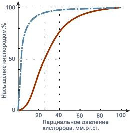
\includegraphics[width=6cm]{figures/krivye-hb-mb.pdf}
	\caption{Кривые насыщения молекулярным кислородом миоглобина (1) и гемоглобина (2) \cite{Volkenshtejn1988}}
	\label{gemoMioglobins}
\end{figure}

Кривая оксигенации миоглобина и гемоглобина.

Гемоглобину легче отдать кислород миоглобину в силу двухстадийности!


Миоглобин является одиночной полипептидной цепью, состоит из 153 аминокислот с молекулярной массой 17 кДа и по структуре сходен с $\beta$-цепью гемоглобина. Белок локализован в мышечной ткани. Миоглобин обладает более высоким сродством к кислороду по сравнению с гемоглобином. Это свойство обуславливает функцию миоглобина --- депонирование кислорода в мышечной клетке и использование его только при значительном уменьшении парциального давления $O_2$ в мышце (до 1-2 мм рт.ст).

Кривые насыщения кислородом показывают отличия миоглобина и гемоглобина:

-- одно и то же 50\%-е насыщение достигается при совершенно разных концентрациях кислорода --- около 26 мм рт.ст. для гемоглобина и 5 мм рт.ст. для миоглобина,
-- при физиологическом парциальном давлении кислорода от 26 до 40 мм рт.ст. гемоглобин насыщен на 50-80\%, тогда как миоглобин --- почти на 100\%.

Таким образом, миоглобин остается оксигенированным до того момента, пока количество кислорода в клетке не снизится до предельных величин. Только после этого начинается отдача кислорода для реакций метаболизма.




{\bf Один из методов регуляции. Ферменты синтезируются в другой форме!}

Как по кривой зависимости от концентрации субстрата, определить конкурентное или неконкурентное ингибирование. Конкурентное ингибирование снимается большими концентрациями субстрата! А неконкурентное не снимается, поскольку сайт заблокирован!


Но фермент машина тоже не может все объяснить... ферменты энтропийного катализа, не представляют собой машины. Поэтому полезны разные модели.




\newpage
%%%%%%%%%%%%%%%%%%%%%%%%%%%%%%%%%%%%%%%%%%%%%%%%%%%%%%%%%%%%%%%%%%%%%%%%%%%%%%%%%%%%%%%%
\section{Концепция <<фермент-машина>> по Д.С. Чернавскому}
{\it Положения, лежащие в основе концепции <<фермент-машина>>. Классические гипотезы о механизмах ферментативных реакций и данная концепция. Область применимости концепции <<фермент-машина>>.}

\subsection{Положения, лежащие в основе концепции <<фермент-машина>>}

Дыба классическая и дыба по Филькенштейну и Птицину.

А фермент машина объясняет аллостерическую регуляцию, то что не может объяснить ключ замок и дыба.

Но фермент машина тоже не может все объяснить... ферменты энтропийного катализа, не представляют собой машины. Поэтому полезны разные модели.



\newpage
%%%%%%%%%%%%%%%%%%%%%%%%%%%%%%%%%%%%%%%%%%%%%%%%%%%%%%%%%%%%%%%%%%%%%%%%%%%%%%%%%%%%%%%%
\section{Биологические мембраны как составная часть клеточной оболочки}
{\it Амфифильные вещества и образование мембранных структур. Молекулярная организация биологических мембран. Фазовые переходы в мембранах. Особенности структуры мембранных белков. Меж- и внутримолекулярные взаимодействия в мембранах. Проблема локализации и необходимой ориентации белков в мембранах.}

\subsection{Амфифильные вещества и образование мембранных структур}

Живое --- есть фазово-обособленная система...



\newpage
%%%%%%%%%%%%%%%%%%%%%%%%%%%%%%%%%%%%%%%%%%%%%%%%%%%%%%%%%%%%%%%%%%%%%%%%%%%%%%%%%%%%%%%%
\section{Биологические механохимические машины}
{\it Ферменты. АТФ-синтетаза. Бактериальный мотор. Броуновская <<трещотка>>. Мышцы. Механохимическая машина Качальского и Оплатки.}

\subsection{Ферменты. АТФ-синтетаза}

Молекула АТР является универсальным источником энергии для большинства многочисленных биохимических, механохимических и транспортных процессов, которые протекают внутри живой клетки. Она работает как вращающаяся машина, ее ротор вращается при прохождении через нее электрического тока, создаваемого не движением электронов, а потоком протонов.

{\bf АТФ-синтаза} --- это обратимая молекулярная машина, которая способна катализировать как синтез, так и гидролиз АТР.

\par\bigskip {\bf Строение АТФ-синтазы}

Способность синтезировать АТФ --- это свойство единого комплекса $F_0F_1$.

{\bf Комплекс $F_1$} --- фрагмент АТФ-синтазы, выступающий из мембраны в виде сферического образования.
 \begin{itemize}
 \item[-] ориентирован в водную фазу;
 \item[-] состоит из девяти субъединиц пяти типов(3$\alpha$, 3$\beta$, $\gamma$, $\delta$ и $\varepsilon$);
 \item[-] имеет вид слегка приплюснутого шара, в центре которого находится субъединица $\gamma$, образована двумя протяженными полипептидными цепями; нижняя ее часть выступает из шара на 3 нм в сторону мембранного комплекса $F_0$;
 \item[-] имеет вид слегка приплюснутого шара, в центре которого находится субъединица $\gamma$, образована двумя протяженными полипептидными цепями; нижняя ее часть выступает из шара на 3 нм в сторону мембранного комплекса $F_0$;
 \item[-] минорная субъединица $\varepsilon$ находится внутри ансамбля $(\alpha \beta)_3$; она связана с субъединицей $\gamma$; 
 \item[-] субъединицы $\gamma$ и $\varepsilon$ подвижны; вращаются внутри неподвижного комплекса $(\alpha \beta)_3$.
 \end{itemize}
 
\begin{figure}[ht] \center
\begin{multicols}{2}
\hfill
 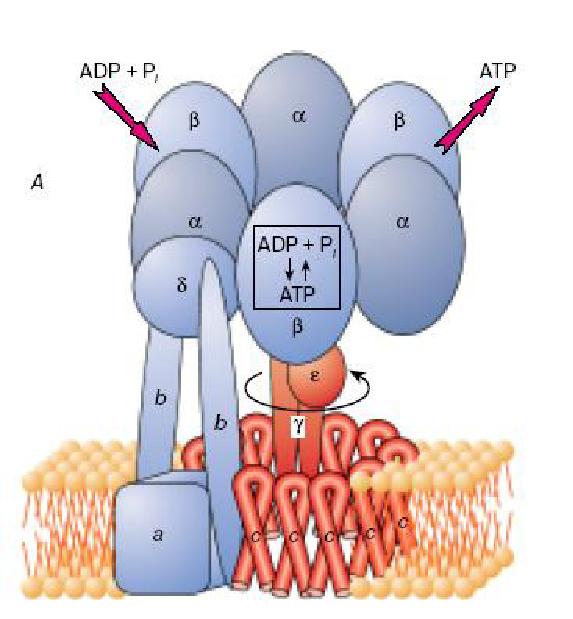
\includegraphics[width=6cm]{figures/fig_5_7_1.pdf}
 \hfill
 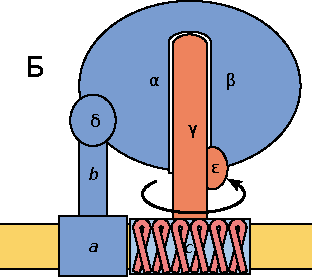
\includegraphics[width=5cm]{figures/fig_5_7_2.pdf}
  \hfill
  \end{multicols}
\end{figure}

{\bf Мембранный комплекс $F_0$} --- мембранная часть АТФ-синтазы, гидрофобный белковый комплекс.

\begin{itemize}
 \item[-] основание, которое удерживает АТФ-синтазу в мембране;
 \item[-] включает в себя протонный канал (ионы водорода переносятся через АТФ-синтазу);
 \item[-] белковая субъединица типа a (гидрофобна, почти полностью погружена в мембрану);
 \item[-] две копии субъединицы $b$ (сравнительно короткий участок, погруженный в мембрану; остальная часть заметно выступает из мембраны в сторону комплекса $F_1$ и закрепляется за расположенную на его поверхности субъединицу $\delta$);
 \item[-] большое количество более мелкой субъединицы $c$ (сравнительно небольшой белок, состоящий из двух гидрофобных $\alpha$--спиралей; образуют единый ансамбль, имеющий форму цилиндра, погруженного в мембрану).
\end{itemize}
 
$F_0$ и $F_1$ соединены друг с другом двумя перемычками. Одна из них представляет собой неподвижный <<кронштейн>> (субъединицы $b$), а другая --- <<ножка>> --- является подвижной субъединицей $\gamma$ ротора.

\par\bigskip {\bf Ротор и статор АТФ-синтазы}

{\bf Статор} --- шарообразный гексамер (3$\alpha$ и 3$\beta$); субъединицы $\delta$, $a$ и $b$ мембранного комплекса $F_0$; $b$ --- кронштейн, связывающий субъединицы $F_0$ и $F_1$; гидрофобное кольцо из субъединицы $c$. 

{\bf Ротор:}

\begin{itemize}
 \item[-] субъединицы $\gamma$ (внутри комплекса $(\alpha \beta)_3$, заметно выступает и соединяется с $c$);
 \item[-] $\varepsilon$ (препятствует свободному вращению ротора, зацепляясь за неровности внутри полости, образованной субъединицами $\alpha$ и $\beta$). 
\end{itemize}
 
Поворот $\gamma$ вызывает одновременное изменение конформации всех трех каталитических субъединиц $\beta$, что в конечном итоге обеспечивает работу фермента. 

{\bf Смазка:}

Центральная часть субъединицы $\gamma$ гидрофобна (не содержит заряженных групп, взаимодействие которых с зарядами субъединиц $\alpha$ и $\beta$ создавало бы дополнительное трение, препятствующее вращению $\gamma$). 
Для того, чтобы провернуть ротор внутри статора, и тем самым заставить АТФ-синтазу сделать молекулу АТР, необходим внешний источник энергии (синтез --- энергия ионов водорода, гидролиз --- энергия, запасенная в АТР). 

\par\bigskip {\bf Вращение}

Способы доказательства:

\begin{itemize}
\item[1.] Применение искусственных химических сшивок между субъединицами $\beta$ и $\gamma$ с помощью дисульфидных ($S-S$) мостиков. 
\item[2.] Использование оптического метода, который позволяет изучать подвижность специальной химической метки, присоединенной к субъединице $\gamma$. 
\item[3.] Наблюдение за вращением субъединицы $\gamma$ с помощью флуоресцентного микроскопа. 
\end{itemize}

\begin{figure}[ht] \center
	 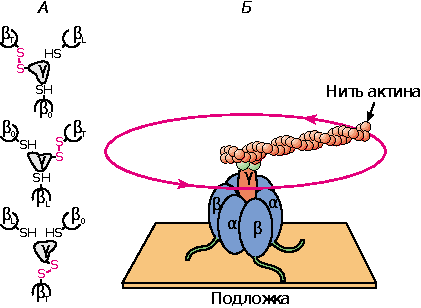
\includegraphics[width=8cm]{figures/fig_5_7_3.pdf}
 \caption{Вращение АТФ-синтазы \cite{Tihonov1999p1}}
\end{figure}

Было показано, что молекула $F_1$ вращает актиновый хвост дискретными скачками с шагом, равным $120^o$. А один скачок --- гидролизом одной молекулы АТР. При этом средняя скорость вращения мотора зависит от нагрузки: чем она выше, тем медленнее крутится мотор. Работа, которую совершает мотор при повороте актинового хвоста на $120^o$, почти в точности равна энергии, запасенной в молекуле АТР. Это означает, что КПД работы мотора примерно 100\%. 

\par\bigskip {\bf Протонный канал АТФ-синтазы}

Протонный канал расположен на границе между субъединицами $a$ и $c$. Путь переноса протонов включает следующие структурные элементы.

\begin{itemize}
\item[1.] Два протонных <<полуканала>>, расположенных в мембранной части АТФ-синтазы. Один из них обеспечивает поступление протонов к определенным функциональным группам $F_0$, расположенным внутри мотора. Другой --- обеспечивает выход протонов в область с пониженной концентрацией ионов водорода (щелочной резервуар). Полуканалы не связаны друг с другом непосредственно, поскольку они расположены несоосно, то есть смещены друг относительно друга.
\item[2.] Кольцо из субъединиц $c$. Каждая из этих субъединиц в своей центральной части содержит протонируемую карбоксильную группу ($R-COOH$), которая способна присоединять протон из кислотной области ($R-COO^- + H^+ \to R-COOH$) и отдавать его в щелочную область ($R-COOH \ to R-COO^- + H^+$) через соответствующие протонные каналы. 
\end{itemize}

\begin{figure}[ht] \center
	 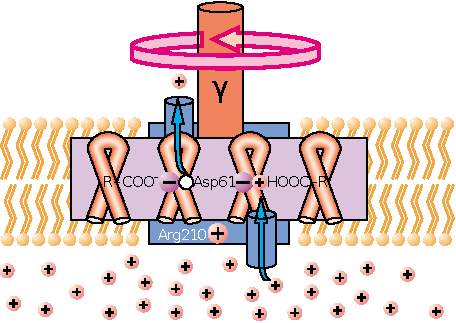
\includegraphics[width=8cm]{figures/fig_5_7_4.pdf}
 \caption{Протонный канал АТФ-синтазы \cite{Tihonov1999p1}}
\end{figure}

Движение протонов может происходить также под действием разности электрических потенциалов. Положительный потенциал со стороны нижнего полуканала будет способствовать протонированию, а отрицательный потенциал со стороны верхнего полуканала --- депротонированию карбоксильных групп субъединиц $c$. Поддерживая на мембране достаточно высокую разность электрических потенциалов ($\Delta \varphi$) можно заставить мотор вращаться даже при одинаковых концентрациях ионов водорода по обе стороны мембраны. Как правило, для этого достаточно создать на мембране разность потенциалов $\Delta \varphi$ порядка 180--200 мВ. 



\subsection{Бактериальный мотор}

Бактерии плавают с помощью жгутиков, вращаемых электромоторами. Их может быть несколько. Когда жгутики начинают синхронно вращаться против часовой стрелки, они сплетаются в единый пучок, который образует своеобразный пропеллер. После того как направление вращения жгутиков изменяется на противоположное, пучок расплетается и бактерия останавливается.

Электромоторы бактерий в качестве источника энергии используют разность протонных потенциалов на цитоплазматической мембране.

\begin{figure}[ht] \center
	 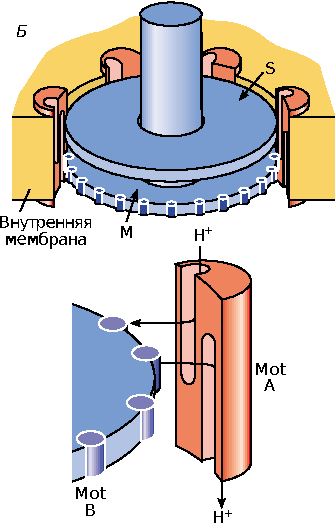
\includegraphics[width=5cm]{figures/fig_5_7_5.pdf}
 \caption{Бактериальный мотор \cite{Tihonov1999p1}}
\end{figure}

Мотор состоит из ротора, статора и некоторых вспомогательных белковых субъединиц, выполняющих роль подшипника, внутри которого вращается стержень ротора. Важными узлами бактериального электромотора являются два соосных диска ($M-$ и $S-$ диски), центры которых соединены с вращающимся стержнем, выступающим наружу. На периферии диска $M$ находятся многочисленные копии белка $Mot\ B$. Несколько копий белка $Mot\ A$, входящего в состав статора, встроены в мембрану и примыкают к краям дисков $M-$ и $S-$.

Вращающий момент возникает за счет взаимодействия субъединиц $Mot\ B$ с белковыми субъединицами $Mot\ A$, расположенными на статоре электромотора. Подобно протонному каналу АТФ-синтазы, путь переноса протонов через мембрану проходит через протонные полуканалы субъединиц $Mot\ A$ и $Mot\ B$.

Один полный оборот ротора связан с переносом через мембрану около 1000 протонов. Бактерии плавают со средней скоростью около 25 мкм/с, но некоторые виды могут двигаться поступательно со скоростью больше 100 мкм/с. Электромоторы, которые могут так быстро вращать жгутики бактерий, очень экономичны --- они потребляют не более 1\% энергетических ресурсов клетки.

\subsection{Броуновская <<трещотка>>}

Как амеба вытягивает ложноножки? Во время существования клеточная мембрана испытывает различного рода колебания, т.е. вибрирует. И, как только в одном месте мембраны происходит вздутие, микротрубочки тут же как бы подпирают мембрану и образуется вздутие (пузырек) (угол 70 градусов между ножками вилки). Выбрасывание псевдоподий связано с этим же механизмом. 



\subsection{Мышцы}


{\bf Модель скользящих нитей}

Саркомер --- структурно-функциональная единица миофибрилл, располагается вдоль мышечных волокон, состоит из параллельных рядов толстых и тонких нитей.

$Z$ --- граница. Между ними видны горизонтальные нити сократительного аппарата. От $Z$--линий отходят тонкие нити --- светлые полосы I. В центральной части саркомера расположены толстые нити --- темные полосы $A$. $B$ середине каждой полосы $A$ видна более светлая полоса $H$. Более светлая полоса (зона $H$) соответствует участку саркомера, где толстые нити не перекрываются с тонкими нитями. Толстые нити состоят из молекул миозина \cite{Tihonov1999p2}.

\begin{figure}[ht] \center
 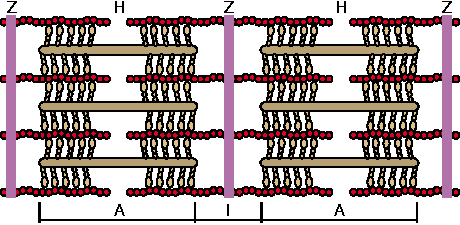
\includegraphics[width=8cm]{figures/fig_5_7_6.pdf}
\end{figure}

Тонкие нити содержат белки трех типов: актин, тропомиозин и тропониновый комплекс. Если посмотреть на поперечный срез саркомера в области, где соседствуют толстые и тонкие нити (темный участок полосы А), то можно увидеть, что каждая тонкая нить окружена тремя толстыми нитями, а каждая толстая нить окружена шестью тонкими нитями. При взаимодействии заполняют щели между соседними толстыми и тонкими нитями.

В основе модели скользящих нитей лежат следующие факты: 

\begin{itemize}
\item[a)] при сокращении мышцы длины толстых и тонких нитей саркомера не изменяются;
\item[b)] cаркомер укорачивается за счет перекрывания толстых и тонких нитей, которые скользят друг относительно друга во время сокращения мышцы. Это проявляется в том, что при сокращении мышцы полосы H и I укорачиваются;
\item[c)] сила, развиваемая мышцей, создается в процессе движения соседних нитей.
\end{itemize}

Скольжение толстых и тонких нитей друг относительно друга совершается за счет энергии, выделяемой при гидролизе АТР до ADP и неорганического фосфата ($P_i$). 
Актин и миозин образуют актомиозиновый комплекс. 

\par\bigskip {\bf Строение толстых и тонких нитей}

\par\bigskip {\bf Толстые нити}

Элементарная структурная единица --- молекула миозина.

Миозин скелетных мышц (миозин класса II) представляет собой димер, каждый мономер которого состоит из одной тяжелой цепи и двух легких цепей. На одном конце тяжелой цепи полипептидная цепь свернута в виде глобулы, образующей <<головку>> миозина (фрагмент S1). С помощью более тонкой шейки (фрагмент S2) головка миозина соединяется с длинным хвостом, который образован протяженной полипептидной цепью, уложенной в виде $\alpha$--спирали. Хвосты двух мономерных единиц сплетены друг с другом. В ходе сокращения наклон головок миозина относительно его хвост изменяется, в результате чего обеспечивается взаимодействие миозина с актином. 

\begin{figure}[ht] \center
\label{kinez}
	 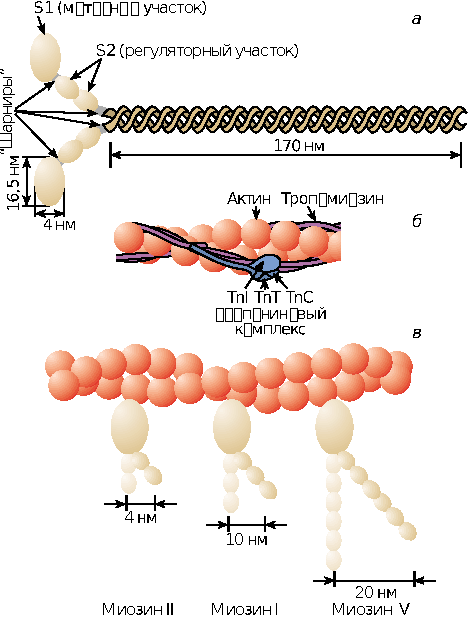
\includegraphics[width=5cm]{figures/fig_5_7_7.pdf}
 \caption{Строение молекулы миозина и тонкой нити~\cite{Tihonov1999p2}}
\end{figure}

Наличие молекулярных шарниров дает возможность фрагменту S1 присоединяться и отсоединяться от нити актина, а также изменять свою ориентацию в ходе сократительного цикла. 

Молекулы миозина в мышцах работают не поодиночке, а образуют толстые жгуты из сплетенных друг с другом димеров. В саркомерах поперечнополосатых мышц каждая толстая нить состоит приблизительно из 300 сплетенных димеров миозина. 

\par\bigskip {\bf Тонкие нити}

Тонкие нити мышечных волокон состоят из нескольких белков (рис. \ref{kinez}). Основной составляющей тонких нитей является G--актин, присутствующий в них в форме вытянутых полимерных нитей. Его мономеры могут связываться друг с другом, образуя вытянутые линейные полимеры (F-актин) микрофиламенты.

Тонкие нити также другие белки --- тропомиозин и три белка тропонинового комплекса, которые играют решающую роль в регуляции взаимодействия миозина с актином. 

\begin{figure}[ht] \center
	 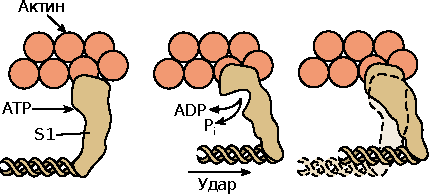
\includegraphics[width=7cm]{figures/fig_5_7_8.pdf}
 \end{figure}

\par\bigskip {\bf Акт мышечного сокращения}

В покоящейся мышце тропомиозин и белки тропонинового комплекса препятствуют взаимодействию головок миозина с нитью актина. Активация актомиозинового комплекса инициируется ионами $Ca^{2+}$. 
Тянущая сила, вызывающая движение молекул миозина вдоль нитей актина, возникает за счет структурных изменений, происходящих в каталитическом центре миозина после гидролиза молекулы AТP. 

Структурные перестройки каталитического центра S1, дают небольшое смещение атомов в активном центре, вызывают значительное перемещение хвоста миозина (3--5 нм для миозина скелетных мышц), т.к. рычаг имеет неравные плечи (точка опоры существенно ближе к активному центру S1, чем конец шейки, соединяющийся с хвостом миозиновой нити). 

\par\bigskip {\bf Рабочий цикл актомиозинового комплекса}

В процессе сокращения мышцы каждая головка миозина совершает многократные повороты, периодически изменяя угол своего наклона относительно нити актина.

\begin{figure}[ht] \center
	 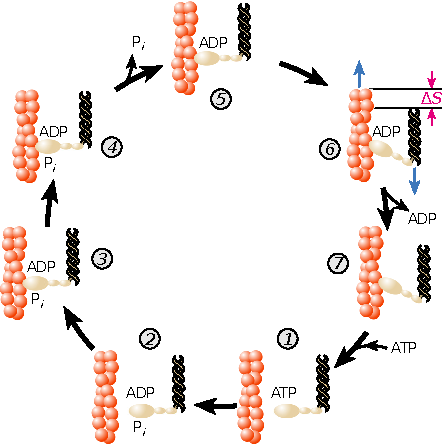
\includegraphics[width=7cm]{figures/fig_5_7_9.pdf}
	 \caption{Цикл актомиозинового комплекса~\cite{Tihonov1999p2}}
\end{figure}


{\bf (1 $\to$ 2)} --- расслабленная мышца, миозиновый мостик отделен от актиновой цепи, молекула АТР расщепляется на ADP и Pi в каталитическом центре;

{\bf (3)} --- за гидролизом молекулы АТР происходит присоединение головки миозина к актиновой нити: сначала образуется слабая связь;

{\bf (4)} --- возникает более прочная связь, вращательная подвижность миозинового мостика становится ограниченной;

{\bf (4 $\to$ 5)} --- прочное связывание головки миозина с актином инициирует освобождение фосфата Рi из активного центра, происходит увеличение сродства миозина к актину;

{\bf (5 $\to$ 6)} --- появляется сила, вызывающая поворот мостика в сторону хвоста, вместе с поворотом мостика смещается вдоль нити актина хвост миозина, происходит сокращение длины саркомера. 

{\bf (7 $\to$ 1)} --- после смещения головки миозина, инициированного диссоциацией фосфата, молекула ADP диссоциирует из каталитического центра, а ее место занимает новая молекула АТР, отсоединение головки миозина от актина.

В результате многократно повторяющихся циклов гидролиза АТР возникает направленное скольжение нитей миозина и актина друг относительно друга.

\par\bigskip {\bf Кооперативная деятельность миозина}

В мышечных волокнах молекулы миозина работают не индивидуально, а кооперативно, в составе крупных макромолекулярных ансамблей. Во время сокращения мышцы лишь сравнительно небольшая часть мостиков (10--15\%) одновременно находится в контакте с окружающими их нитями актина (картинка про бревно). 

Это значит, что каждый из мостиков большую часть времени проводит в свободном состоянии, когда он непосредственно не создает тянущей силы. При этом молекулы миозина, у которых мостики отсоединены от актиновых нитей, во время сокращения саркомера перемещаются вместе с остальными молекулами миозинового жгута. Это значит, что каждый мостик не просто шагает вдоль нити, равномерно ступая между соседними звеньямиактиновой цепи, а как бы прыгает вдоль нее. Таким образом, сокращение мышечных волокон обеспечивается за счет кооперативной работы большого количества молекул миозина, собранных в толстые нити. 

\par\bigskip {\bf Кинезин}

Кинезин работает как переносчик различных органелл (митохондрии, лизосомы) и супермолекулярных частиц. Молекула кинезина --- это димер, образованный двумя одинаковыми полипептидными цепями. С одной стороны каждой полипептидной цепи кинезина формируется глобулярная головка, соединенная со сравнительно длинным хвостом. Хвосты двух мономерных цепей сплетены вместе, а наклоненные в разные стороны головки образуют своеобразную рогатину, которая непосредственно взаимодействует с глобулярными мономерами микротрубочки, вдоль которой перемещается кинезин. 

\begin{figure}[ht] \center
	 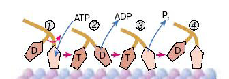
\includegraphics[width=5cm]{figures/fig_5_7_10.pdf}
	 \caption{Схема движения кинезина~\cite{Tihonov1999p2}}
\end{figure}

Головки кинезина попеременно связываются с мономерными звеньями микротрубочки. В ходе структурных перестроек моторных участков кинезина угол наклона головок относительно микротрубочки изменяется, вследствие чего кинезиновый димер смещается вдоль микротрубочки. Сила, развиваемая одной молекулой кинезина, составляет величину $F \approx $6 пН. Если бы такой мощностью в расчете на единицу массы обладали автомобильные моторы, то они могли бы легко разгонять машины до скоростей, существенно превышающих скорость звука. Коэффициент полезного действия кинезинового мотора также велик. Кинезин может совершать перемещения на очень большие расстояния (до 1 мм).



\subsection{Механохимическая машина Качальского и Оплатки}

Слабо сшитые полиэлектролитные гели способны трансформировать химическую энергию в механическую работу. Представим себе полианионный гель, изготовленный, например, из полиметакриловой кислоты и набухший в воде при нейтральном $pH$. Добавление щелочи к такому гелю увеличит степень ионизации кислотных групп, их взаимное эклектростатическое отталкивание и, следовательно степень набухания. Изменение объема геля можно использовать для совершения работы. Если изготовить из слабо сшитого полиэлекторлита волокно, то оно будет удлиняться или укорачиваться при добавлении щелочи или кислоты и производить соответствующую работу. Напротив, механическое растяжение такого волокна приводит к изменению ионного состава омывающей жидкости. Аналогичные процессы происходят в результате изменения ионной силы --- внедрения в набухший полиэлектролит нейтральной соли. 

\begin{figure}[ht] \center
	 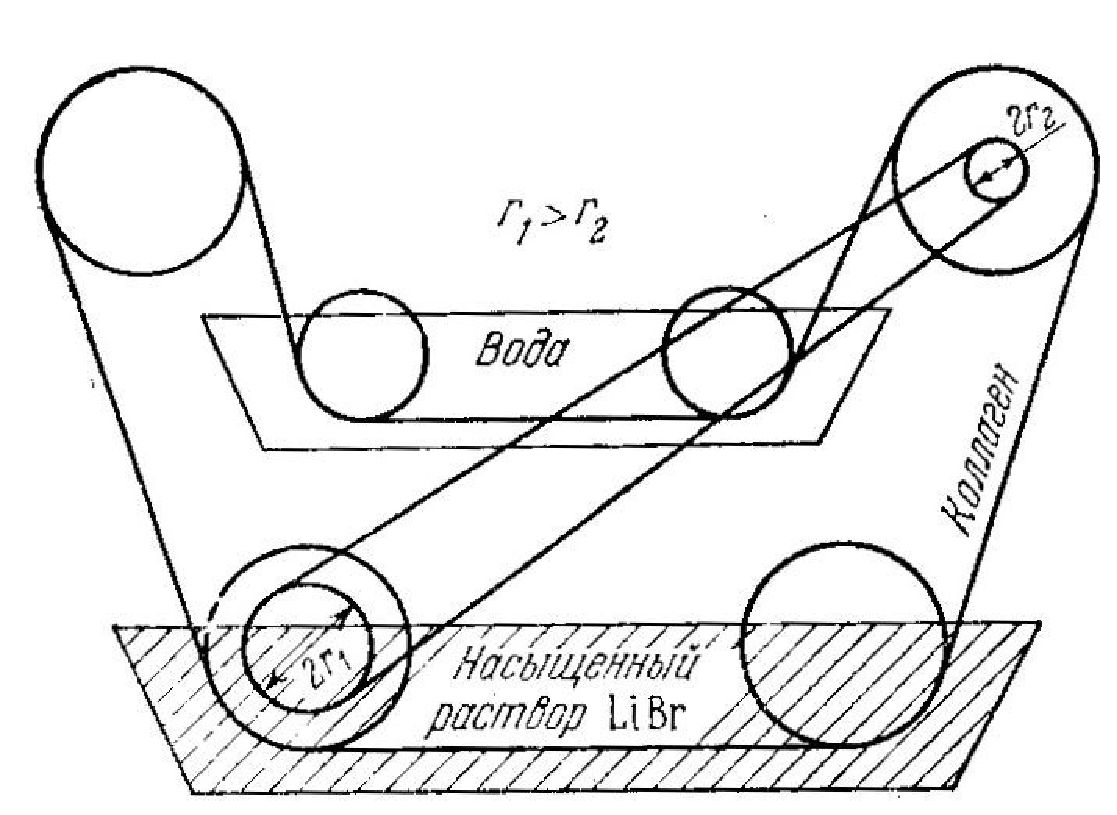
\includegraphics[width=7cm]{figures/fig_5_7_11.pdf}
	 \caption{Схема машины Качальского и Оплатки}
\end{figure}

Качальский и Оплатка построили непрерывно работающую машину, в которой полиэлектролитное волокно (коллаген) попеременно погружается в раствор соли и в чистую воду. Работа машины прекращается, когда в результате переноса малых ионов волокном в воду химические потенциалы обоих резервуаров выравниваются. Такая машина может быть пущена в обратную сторону за счет внешнего источника энергии.

Полианионное волокно Качальского и Оплатки сокращается при понижении $pH$, скажем, при добавлении $HCl$. 



Новые способы движения бактерий.




\newpage
%%%%%%%%%%%%%%%%%%%%%%%%%%%%%%%%%%%%%%%%%%%%%%%%%%%%%%%%%%%%%%%%%%%%%%%%%%%%%%%%%%%%%%%%
\section{Трансформация энергии в биомембранах}
{\it АТР как универсальный химический переносчик энергии для сопряжения химических реакций друг с другом и другими клеточными процессами. Перенос электронов и трансформация энергии в биомембранах. Электрон-транспортные цепи. Механизмы генерации электрохимического потенциала. Окислительное фосфорилирование и хемиосмотическая теория Митчелла.}

\subsection{АТР как универсальный химический переносчик энергии для сопряжения химических реакций друг с другом и другими клеточными процессами}

Рубин!

Для гетеротрофных клеток источником свободной энергии, получаемой в химической форме, служит процесс расщепления, или катаболизм, пищевых молекул (в основном углеводов и жиров). Эту энергию клетки используют в следующих целях: 
1) для синтеза биомолекул из молекул-предшественников небольшого размера; 
2) для выполнения механической работы, например мышечного сокращения, 
3) для переноса веществ через мембраны против градиента концентрации и 
4) Для обеспечения точной передачи информации. Главным связующим звеном между клеточными реакциями, идущими с выделением и с потреблением энергии, служит АТР. При расщеплении высокоэнергетического клеточного топлива часть содержащейся в этом топливе свободной энергии используется для синтеза АТР из ADP и неорганического фосфата Р. Позже АТР, распадаясь на ADP и фосфат, отдает значительное количество своей химической энергии тем процессам, для которых энергия необходима. АТР - переносчик химической энергии, от клеточных процессов, сопровождающихся выделением энергии, с процессами, в которых энергия потребляется.

Процессы преобразования энергии при электронном транспорте в мембранах митохондрий, хлоропластов, хроматофоров и некоторых бактерий обладают фундаментальным сходством. Во всех этих системах реализуется единый принцип сопряжения переноса электронов по цепи электронного транспорта с синтезом АТФ. Этот принцип иллюстрирует рис. 1, на котором показано, что перенос электронов по электронтранспортной цепи (1) приводит к переносу протонов через гидрофобный барьер мембраны. В результате энергия окислительно-восстановительных реакций трансформируется в трансмембранную разность электрохимических потенциалов ионов водорода (), которая используется АТФ-синтетазой (2) для синтеза АТФ из АДФ и Фн.

Рис. 1. Схема превращения энергии в биомембранах. Цепь электронного транспорта (1), используя энергию окислительно-восстановительных реакций, транспортирует протоны через мембрану против их электрохимического потенциала. 

Стадии превращения энергии в метахондриях:
Образование доноров электронов для ЦЭТ (НАДН, сукцинат и др.),
Перенос электронов по ЦЭТ от НАДН и сукцината к кислороду, сопряженный с образованием трансмембранной разности электрохимических потенциалов ионов водорода (),
Использование для синтеза АТФ из АДФ и Фн.

Все стадии, кроме первой, протекают во внутренней мембране митохондрий. Основной энергетической функцией ЦЭТ митохондрий является использование энергии редокс-реакций для синтеза АТФ, причем образующаяся в процессе этих реакций может непосредственно использоваться для совершения химической и осмотической работы и других процессов.
Известно около 20 переносчиков электронов, составляющих ЦЭТ митохондрий. К ним относятся NADH, флавины, убихинон, цитохромы, которые содержат гемовую(железо-порфириновую) простетическую группу. Цитохромы подразделяются на три основных класса (а, , с) согласно типу гема, а также их характерному спектру поглощения в восстановленной форме.
Дыхательная цепь переноса электронов является частью окисл. фосфорилирования
В каждом обороте цикла лимонной кислоты специфичные дегидрогеназы отщепляют от изоцитрата, а-кетоглутарата. сукцината и малата четыре пары атомов водорода. Они в определенной точке отдают свои электроны в цепь переноса электронов и превращаются таким образом в ионы Н+, которые поступают в водную среду. Электроны, переходя от одного переносчика к другому, достигают в конце концов цитохрома аа3, или цитохромоксидазы, при участии которой они и передаются на кислород --- конечный акцептор эл-ов у аэробных организмов.

Поток электронов по дыхательной цепи возможен благодаря тому, что он сопровождается уменьшением свободной энергии. При переносе двух электронов от NADH на кислород изменение стандартной свободной энергии составляет --- 52,6 ккал.

Стадии переноса электронов:
Кофермент NAD+ выполняет коллекторную функцию --- собирает пары восстановительных эквивалентов, поступающих от разных субстратов в одной молекулярной форме NADH.
Пара восстановительных эквивалентов (электронов, гидрид-ионов и т.д.) переносится от NADH к NADH-дегидрогеназе, находящейся во внутренней митохондриальной мембране. При этом ее простетическая группа FMN восстанавливается.

В [$Fe(II)$ -- $Fe(III)$] --- циклах, связанных с изменением валентности, атомы железо-серных центров передают восстановительные эквиваленты от восстановленной простетической группы FMNH2 на следующий переносчик дыхательной цепи --- убихинон Q (кофермент Q), который восстанавливается до QH2. Убихинон передает электроны на цепь цитохромов b®с1®с®а ® а3.

Цитохромы --- железосодержащие белки, окрашенные в красный или коричневый цвет. Существует три класса а, b, с, различаются по спектрам поглощения. Каждый из цитохромов, находясь в окисной форме [$Fe(III)$], присоединяет один электрон и переходит в закисную форму [$Fe(II)$].

Хемиосмотическая гипотеза сформулирована английским биохимиком Питером Митчелом. Функция переноса электронов, происходящего во внутренней митохондриальной мембране, заключается в том, чтобы откачивать ионы Н+ из матрикса митох-ий в наружную среду и таким образом создавать между двумя водными фазами, которые разделяет эта мембрана, градиент конц. ионов Н+ с более кислым значением снаружи. Этот же процесс ведет к появлению трансмембранного эл. потенциала --- наружная сторона мембраны оказывается электроположительной. Ионы Н+ из окружающей среды вновь устремляются внутрь, т.е. митохондриальный матрикс, на этот раз по электрохимическому градиенту через специальные поры в молекуле F0F1-АТРазы. Этот переход ионов Н+ из зоны с более высокой в зону с более низкой их концентрацией сопровождается выделением свободной энергии, за счет которой и синтезируется АТР. Таким образом, хемиосмотическая гипотеза предполагает, что между митохондрией и окружающей ее средой совершается непрерывный круговорот ионов Н+, движущей силой которого является перенос электронов.




\chapter{Природа биологических и химических сигналов}

%%%%%%%%%%%%%%%%%%%%%%%%%%%%%%%%%%%%%%%%%%%%%%%%%%%%%%%%%%%%%%%%%%%%%%%%%%%%%%%%%%%%%%%%
\section{Транспорт ионов в возбудимых мембранах и распространение нервного импульса}
{\it Потенциал действия и потенциал покоя. Генерация импульса. Транспорт ионов в возбудимых мембранах. Ионные токи в модели Ходжкина-Хаксли. Физико-химические и математические модели возбудимых мембран. Распространение нервного импульса.}

\subsection{Потенциал действия и потенциал покоя}

Генерация импульса начинается со слабой деполяризации, или уменьшения отрицательного потенциала внутренней поверхности мембраны, в том месте, где аксон отходит от клеточного тела. Этот небольшой сдвиг потенциала открывает некоторые из натриевых каналов, вызывая тем самым дальнейшее уменьшение потенциала. Этот процесс является самоусиливающимся: поток ионов натрия через мембрану способствует открыванию большего числа каналов и облегчает другим ионам возможность следовать за ними. 

Проникшие в клетку ионы натрия изменяют отрицательный внутренний потенциал мембраны на положительный. Поток ионов натрия внутрь будет ускоряться до тех пор, пока внутренняя поверхность мембраны не станет локально положительной. Изменение знака потенциала приведет к закрыванию натриевых каналов и открыванию калиевых, что позволяет ионам калия выходить наружу. Этот поток восстанавливает потенциал внутри аксона до величины его потенциала покоя, т.е. до $-70$ мВ. Резкий скачок потенциала сначала в положительную, а затем в отрицательную сторону, который выглядит на экране осциллографа как пик (<<спайк>>), и называется <<потенциал действия>> и является электрическим выражением нервного импульса. Поток ионов калия наружу быстро восстановит отрицательный потенциал. Кратковременная реверсия потенциала (от лат. {\it reversio} --- возвращение, возврат), получившая название потенциала действия, сама распространяется по аксону. После короткого рефрактерного периода (франц. {\it réfractaire} --- невосприимчивый) за первым импульсом может следовать второй.

\par\bigskip {\bf Потенциал покоя}

В мембране имеется $Na^+/K^+$--AТФаза, осуществляющая активный перенос ионов $Na^+$ из клетки в обмен на ионы $K^+$. Этот транспорт энергозависим и сопряжен с гидролизом АТФ. За счет работы $Na^+,K^+$--насоса поддерживается неравновесное распределение ионов $Na^+$ и $K^+$ между клеткой и окружающей средой, поскольку расщепление одной молекулы АТФ обеспечивает перенос трех ионов $Na^+$ из клетки и двух ионов $K^+$ в клетку.

В состоянии покоя мембрана более проницаема для $K^+$, чем для $Na^+$. Вследствие диффузии $K^+$ наружу из аксоплазмы внутреннее содержимое нервного волокна в состоянии покоя заряжено отрицательно по отношению к наружному раствору. Эта постоянная разность потенциалов --- потенциал покоя --- равна 50--70 мВ. Какими факторами определяется это значение? Если бы мембрана была проницаема только для $K^+$, равновесная разность потенциалов достигла бы значения, определяемого уравнением Нернста для калиевого электрода:

\begin{equation}
	\varphi_k=\frac{RT}{F} \ln \frac{[K_0]}{[K_i]},
\end{equation}
где $R$ --- универсальная газовая постоянная, равная 8{,}31 Дж/(моль $\times$ K);\\
$T$ --- абсолютная температура;\\
$F$ ---число Фарадея, равное $96485,35$ Кл/моль.

П\hspace{5pt}р\hspace{5pt}и\hspace{5pt}м\hspace{5pt}е\hspace{5pt}р.
Kонцентрация калия в крови 20 мМ в аксоплазме 400 мМ у кальмара.

\begin{equation}
	\varphi_k=\frac{8,31 \times 3000}{96485,35} \ln \frac{20}{4000}\thickapprox-75 \text{мВ},
\end{equation}

Каналы, проницаемые для $Na^+$ и $Cl^-$, преимущественно закрыты. Ионы фосфата и органические анионы, например белки, практически не могут проходить через мембраны. Но более точно бри низких концентрациях калия потенциал покоя вычисляется по формуле учитывающую диффузию натрия:

\begin{equation}
	\label{613}
	\varphi_K = \frac{RT}{F} \ln \frac{P_k[K_0]+P_{Na}[Na_0]}{P_k[K_i]+P_{Na}[Na_i]},
\end{equation}
где $P_m$---ионная проницаемость для ионов.

Отношение ионных проницаемостей $P_k : P_{Na}=1:0{,}04$


\par\bigskip{\bf Потенциал действия}

Возбуждение нервной клетки под действием химического сигнала (реже электрического импульса) приводит к возникновению потенциала действия. Это означает, что потенциал покоя -60 мВ скачком изменяется на +30 мВ и спустя 1 мс принимает исходное значение. Процесс начинается с открывания $Na^+$--канала (1). Ионы Na+ устремляются в клетку (по градиенту концентрации), что вызывает локальное обращение знака мембранного потенциала (2). При этом $Na^+$--каналы тотчас закрываются, т. е. поток ионов $Na^+$ в клетку длится очень короткое время (3). В связи с изменением мембранного потенциала открываются (на несколько мс) потенциал-управляемые $K^+$--каналы (2) и ионы $K^+$ устремляются в обратном направлении, из клетки. В результате мембранный потенциал принимает первоначальное значение (3), и даже превышает на короткое время по модулю потенциал покоя (4). После этого нервная клетка вновь становится возбудимой.

За один импульс через мембрану проходит небольшая часть ионов $Na^+$ и $K^+$, и концентрационные градиенты обоих ионов сохраняются (в клетке выше уровень $K^+$, а вне клетки выше уровень $Na^+$). Поэтому по мере получения клеткой новых импульсов процесс локального обращения знака мембранного потенциала может повторяться многократно. Распространение потенциала действия по поверхности нервной клетки основано на том, что локальное обращение мембранного потенциала стимулирует открывание соседних потенциал--управляемых ионных каналов, в результате чего возбуждение распространяется в виде деполяризационной волны на всю клетку.


\subsection{?? Транспорт ионов в возбудимых мембранах}


\subsection{Генерация импульса}


Реверсия мембранного потенциала во время развития импульса вызвана тем, что на гребне спайка потенциала действия мембрана избирательно проницаема больше для ионов натрия, так что отношение ионных проницаемостей $P_K:P_{Na}=1:20$. Как видно из формулы \ref{613}, в этих условиях потенциал на мембране приближается к равновесному натриевому потенциалу $\varphi_{Na}$. Разность потенциалов на мембране, проницаемой только для натрия выражается формулой Нернста:

\begin{equation}
	\label{614}
	\varphi_{Na}=\frac{RT}{F} \ln \frac{[Na_0]}{[Na_i]},
\end{equation}

Предельное значение потенциала, вычисленного по формуле \ref{614},равное +55 (??и)В лишь немного превышает экспериментально наблюдаемые значения обращенного потенциала. Эти вводы сохраняются, если воспользоваться для выражения выбранного потенциала более полной формулой, где учтены потоки хлора:

\begin{equation}
\varphi_K=\frac{RT}{F} \ln \frac{P_k[K_0]+P_{Na}[Na_0]+P_{Cl}[Cl_0]}{P_k[K_i]+P_{Na}[Na_i]+P_{Cl}[Cl_i]},
\end{equation}

В состоянии покоя $P_k : P_{Na} : P_{Cl}=1:0{,}04:0{,}45$, а в состоянии возбуждения на пике потенциала действия, когда вновь соблюдается условие нулевого тока через мембрану, $P_k : P_{Na} : P_{Cl}=1:20:0{,}45$

Процесс возбуждения развивается вследствие зависимости проницаемости мембраны для ионов от мембранного потенциала. При достижении критической деполяризации, когда возрастает проницаемость мембраны для $Na^+$, эти ионы устремляются внутрь и вызывают дальнейшую деполяризацию мембраны. Процесс продолжается до тех пор, пока потенциал не сместится до равновесного натриевого потенциала. В этих условиях потоки $Na^+$ наружу и внутрь сравниваются. Затем происходит увеличение проницаемости для $K^+$ и ионы $K^+$ начинают выходить из клетки по градиенту своего электрохимического потенциала. В этом процессе мембрана реполяризуется. Выход $K^+$ прекращается, когда потенциал на мембране приблизится к равновесному калиевому потенциалу. 

После прохождения по аксону одного спайка система возвращается в исходное состояние, за исключением того, что в клетке появился некоторый избыток ионов $Na^+$, вошедших в период деполяризации, и некоторый недостаток ионов $K^+$,вышедших на фазе реполяризации. Изменения внутриклеточной концентрации $Na^+$ и $K^+$, вызванные одиночным потенциалом действия, крайне малы, но могли бы оказаться значительными при многократном прохождении нервных импульсов. Для поддержания постоянного уровня внутриклеточных концентраций $K^+$ и $Na^+$ в клеточной мембране и существует система $Na^+$,$K^+$--насоса, обеспечивающая активное выведение $Na^+$ в обмен на поступление в клетку $K^+$, работающая за счет энергии АТФ. 




\subsection{Ионные токи в модели Ходжкина-Хаксли}

Первая модель распространения электрического импульса вдоль аксона гигантского кальмара была предложена Ходжкиным и Хаксли (1952), и до сих пор является базовой моделью для описания такого типа явлений.

На основе опытов по фиксации напряжения в аксоне кальмара А. Ходжкин и А. Хаксли сформулировали ряд важных принципов.

\begin{itemize}
\item[1.] Перенос $Na^+$ и $K^+$ осуществляется различными невзаимодействующими структурами.
\item[2.] Изменение токов являются следствием изменения проницаемости мембран (для $Na^+$ и $K^+$).
\item[3.] Пропускная способность мембраны управляется электрическим полем.
\end{itemize}

Модель имеет четыре переменные: $\varphi$ (мембранный потенциал), $n$, $m$ и $h$. Три последних переменных характеризуют соответственно проницаемость мембраны для ионов $K^+$, $Na^+$ и других типов ионов. Более современные модели отличаются от модели Ходжкина-Хаксли в основном учетом большего количества типов ионов. Одно из уравнений модели представляет собой закон Кирxгоффа. Остальные уравнения строятся из общефизических соображений и экспериментальных данных. Они имеют вид:

\begin{equation}
	I(t) = C \frac{d \varphi}{dt} + I_j,
\end{equation}

\begin{equation}
	I_j=I_{Na}+I_K+I_L=g_K(\varphi-\varphi_K)n^4+g_{Na}	(\varphi-\varphi_{Na})m^3h+g_L(\varphi-\varphi_L).
\end{equation}

\begin{equation}
\left\{
	\begin{aligned}
	& C \frac{d \varphi}{dt}=-[g_K(\varphi-\varphi_K)n^4+g_{Na}(\varphi-\varphi_{Na})m^3h+g_L(\varphi-\varphi_L)]+I(t);\\
	& \frac{dn}{dt}=\alpha_n(1-n)-\beta_n n; \\
	& \frac{dm}{dt}=\alpha_m(1-m)-\beta_m m; \\
	& \frac{dh}{dt}=\alpha_h(1-h)-\beta_h h. 
	\end{aligned}
\right.
\end{equation}

В первом уравнении системы левая часть этого равенства представляет собой емкостный ток, а правая --- разность между полным током $I(t)$, текущим во внешней цепи, и ионным током, складывающимся из трансмембранного тока $Na^+$, $K^+$ и тока утечки $g_L(\varphi - \varphi_L)$. 

Остальные уравнения системы описывают кинетику перераспределения частиц через мембрану при наложении электрического поля; $\alpha, \beta$ --- константы скорости, зависящие только от мембранного потенциала.

Система имеет стабильное стационарное состояние в отсутствие внешних токов, но когда приложенный импульс тока выше порогового значения, демонстрирует регулярное периодическое возбуждение мембраны.
Модель удается упростить в соответствии с временной иерархией переменных $m$, $n$, $h$. Натриевые токи (величина $m$) протекают гораздо быстрее, чем калиевые (величина $n$), поэтому в соответствии с теоремой Тихонова можно заменить дифференциальные уравнения для натриевой составляющей на алгебраические ($dm/dt=0$). Если считать, что токи утечки протекают еще более медленно ($h = h_0 = const$), модель сводится к системе уравнений для двух переменных:

\begin{equation}
\left\{
	\begin{aligned}
	& \frac{d \varphi}{dt}=f(\varphi)-W+I_0;\\
	& \frac{dW}{dt}=bv-\gamma W, 
	\end{aligned}
\right.
\end{equation}
где $f(\varphi)=\varphi(a-\varphi)(\varphi-1)$, $0 < a < 1$;\\
$b$ и $\gamma$ --- положительные константы;\\
потенциал $V$, $W$ --- характеризует нелинейные свойства проводимости мембраны для всех типов ионов.


\subsection{Физико-химические и математические модели возбудимых мембран}

Среди различных моделей электрической возбудимости клеток особый интерес представляет предложенная в конце 50-х годов Т. Теореллом физико-химическая модельная система, названная мембранным осциллятором. 

Модель представляет собой две ячейки, заполненные электролитом разной концентрации и разделенные мембраной из пористого стекла с фиксированными отрицательными зарядами. 
При пропускании через мембрану тока в ячейках возникает отчетливый сдвиг уровней жидкости, т. е. создается перепад гидростатических давлений. Пока ток не превышает некоторого критического значения, разность потенциалов на мембране и перепад давлений остаются постоянными. Однако после превышения критического значения тока система переходит в автоколебательный режим, при котором разность потенциалов на мембране и разность давлений начинают совершать релаксационные колебания. 

В основе работы мембранного осциллятора лежат электрокинетические явления. Суммарный поток жидкости по капиллярам пористой мембраны представляет собой разность электроосмотического потока (его направление совпадает с направлением электрического поля) и встречно направленного гидродинамического потока. 

Если поток направлен так, что мембрана заполняется концентрированным раствором электролита, то сопротивление мембраны резко снижается, и наоборот, если мембрана заполняется малопроводящим разбавленным раствором, ее сопротивление 
возрастает. 
В зависимости от направления движения жидкости профиль концентрации внутри мембраны приобретает вогнутую или выпуклую форму, соответствующую низкой и высокой концентрации носителей заряда в мембране (рис. \ref{fig.6.1.1}). 
С увеличением скорости течения профиль концентрации в мембране приближается к прямоугольному. При высоких скоростях течения сопротивление мембраны принимает одно из двух предельных значений в зависимости от направления потока раствора (рис. \ref{fig.6.1.2}). 

Скорость течения жидкости $v$ через мембрану зависит от разности давлений $p$ 
и разности потенциалов $\varphi$ ср следующим образом: 

\begin{equation}
\label{pcm}
v=\alpha p-\beta \varphi
\end{equation}

где $\alpha$ и $\beta$ --- коэффициенты пропорциональности. Первый член описывает 
фильтрационное течение через пористую среду, второй --- соответствует 
электроосмотическому потоку. 

\begin{figure}[ht] \center
\begin{multicols}{2}
\hfill
 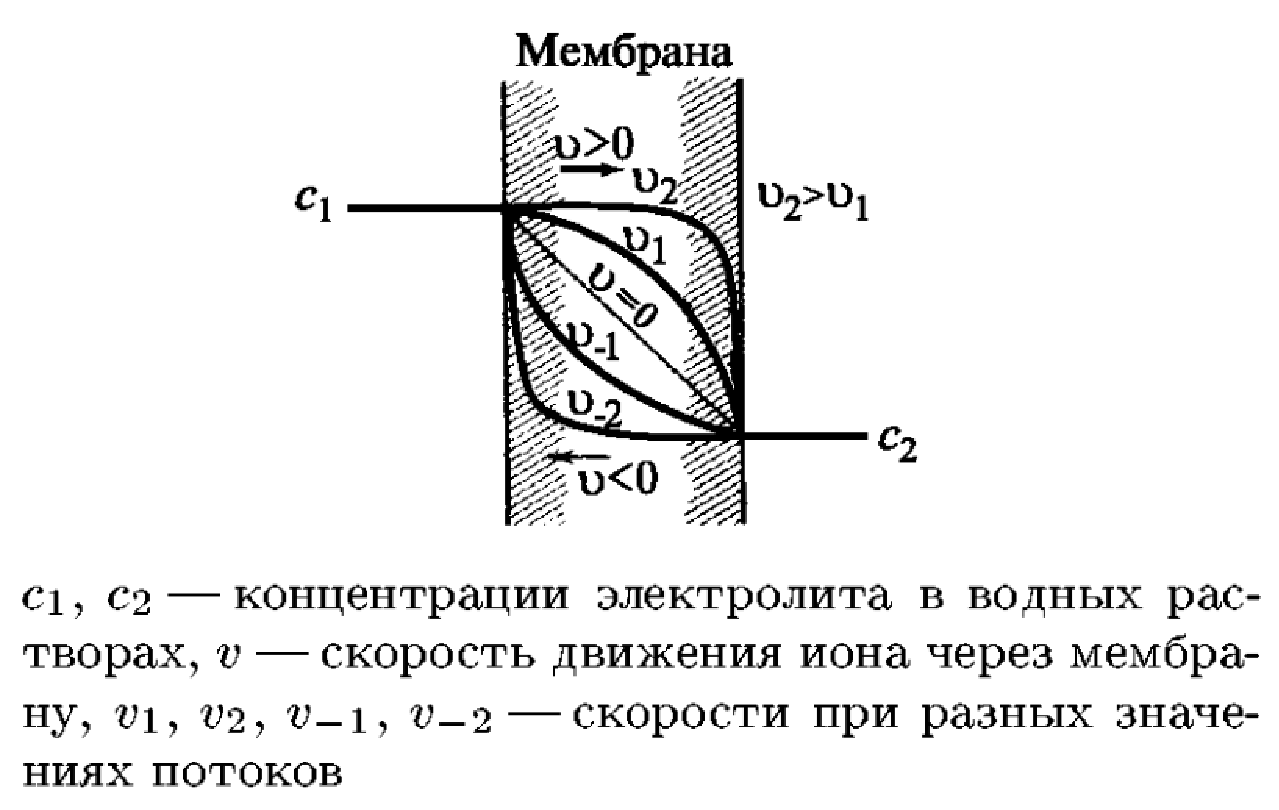
\includegraphics[width=4cm]{figures/fig_6_1_1.pdf}
 \caption{Распределение концентрации ионов внутри мембраны в зависимости от направления и скорости протекания жидкости}
 \label{fig.6.1.1}
 \hfill
 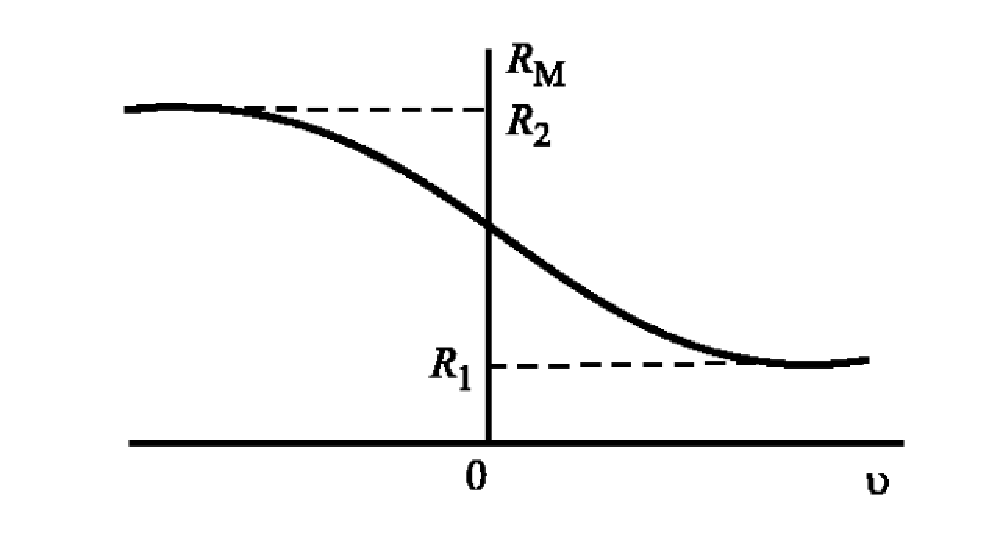
\includegraphics[width=5cm]{figures/fig_6_1_2.pdf}
 \caption{Зависимость сопротивления мембраны $Rm$ от скорости потока жидкости $v$}
 \label{fig.6.1.2}
 \hfill
  \end{multicols}
\end{figure}

\begin{figure}[ht] \center
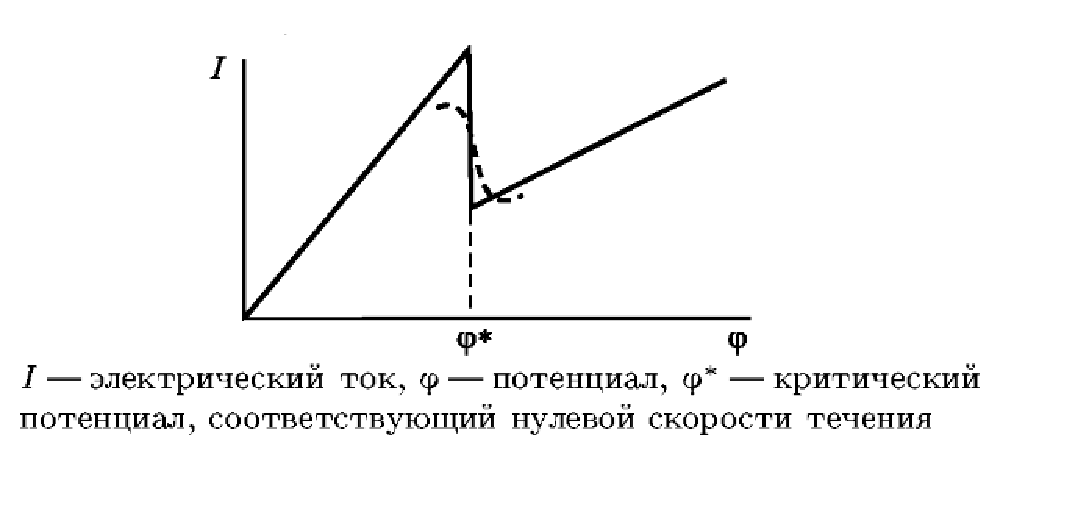
\includegraphics[width=10cm]{figures/fig_6_1_3.pdf}
 \caption{Вольтамперная характеристика мембранного осциллятора (по В. С. Маркину и др., 1981)}
 \label{fig.6.1.3}
\end{figure}

Отсюда следует, что вольтамперная характеристика мембраны состоит из двух линейных участков с резким переходом между ними (рис. \ref{fig.6.1.3}). Наклоны участков определяются сопротивлением электролита в мембране при $c_1$ и $c_2$, а переход между участками происходит при потенциале $\varphi$, соответствующем нулевой скорости течения. Реальная вольтамперная характеристика, полученная методом фиксации потенциала (штриховая на том же рисунке), отличается лишь тем, что вместо резкого перехода имеется довольно крутой участок с отрицательным наклоном. 
 
Существование этого участка создает предпосылки для возникновения колебаний в системе. В некоторых пределах каждому значению тока соответствуют три значения потенциала. Промежуточное значение относится к неустойчивому состоянию, крайние --- к устойчивому, т. е. такая система является триггерной. 

\begin{figure}[ht] \center
\label{fig.6.1.4}
 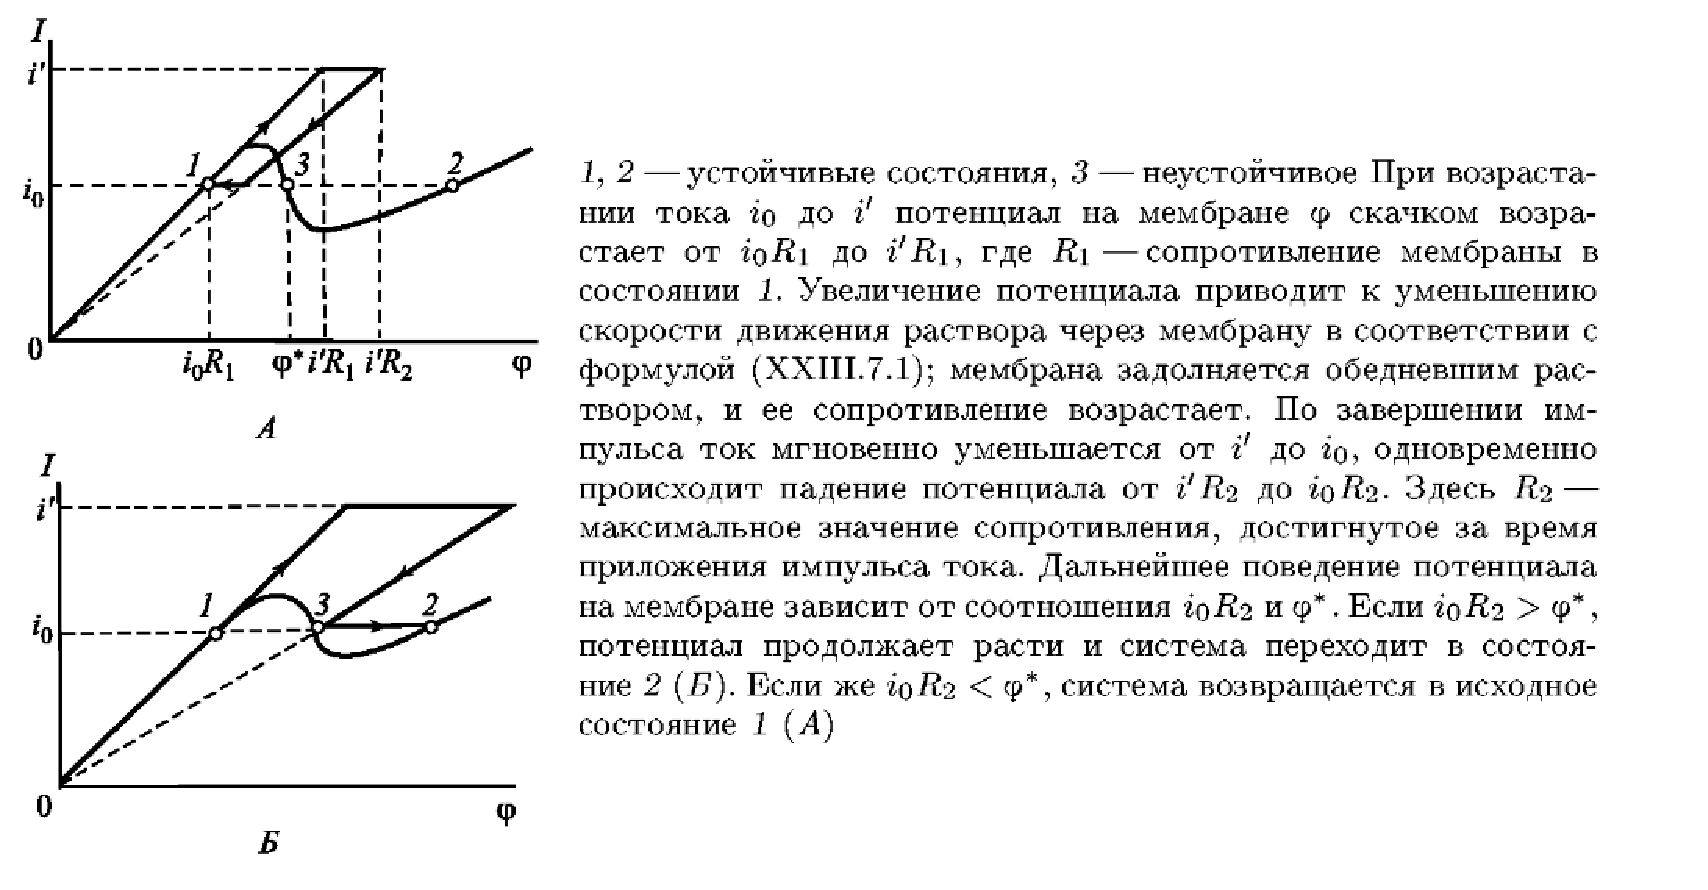
\includegraphics[width=10cm]{figures/fig_6_1_4.pdf}
 \caption{Переход между двумя устойчивыми состояниями в модели Теорелла}
\end{figure}

В том случае, когда в рассматриваемой модели перепад давлений поддерживается на постоянном уровне, с помощью импульсов тока можно переводить систему из одного устойчивого состояния в другое (рис. \ref{fig.6.1.4}). 

В условиях, когда разность давлений не зафиксирована, изменения потенциала на мембране, вызываемые импульсами тока, имеют выраженное сходство с потенциалом действия в аксоне. Амплитуда потенциала в модельной системе составляет около 2 В, а продолжительность достигает нескольких минут. Как следует из уравнения (\ref{pcm}), изменение перепада на мембране не оказывает влияния на крутизну устойчивых участков вольтамперной кривой, а влияет только на значение потенциала $\varphi$, при котором происходит изменение направления движения жидкости, т. е. на положение вертикального участка вольтамперной характеристики. 

Электрохимическая модель, предложенная Теореллом, способна воспроизводить многие свойства нервного волокна, включая проведение возбуждения. 

\subsection{Распространение нервного импульса}

Распространение нервного импульса вдоль волокна происходит без затухания с постоянной скоростью. Внутренняя часть волокна на участке возникновения спайка заряжена положительно, а в соседних участках --- отрицательно. Причем, в направлении, откуда спайк распространяется, отрицательный заряд меньше в силу того, что на восстановление прежней разности потенциалов требуется время (рефрактерный период). Вследствие этого возникает локальный ток между возбужденным и покоящимися участком по направлению движения спайка. Направление тока такого, что он деполяризует часть мембраны перед активным участком, что приводит к возбуждению и возникновению нового спайка. Таким образом, возбуждение передается дальше по волокну.

Скорость распространения устойчивого импульса обратно пропорциональна квадратному корню из диаметра волокна.

В организме нервные волокна объединены в нервные стволы, где каждое волокно может самостоятельно производить возбуждение. Электрическое поле, возникающее при этом в возбужденном волокне, влияет на мембранный потенциал соседних волокон, которые тем самым при некоторых условиях могут также возбуждаться. 




\newpage
%%%%%%%%%%%%%%%%%%%%%%%%%%%%%%%%%%%%%%%%%%%%%%%%%%%%%%%%%%%%%%%%%%%%%%%%%%%%%%%%%%%%%%%%
\section{Пассивный транспорт веществ через мембрану}
{\it Диффузия. Облегченная диффузия. Транспорт ионов. Ионное равновесие на границе раздела фаз. Уравнения электродиффузии Нернста-Планка и их решение.}

\subsection{Диффузия}

{\bf Транспорт неэлектролитов. Диффузия (простая и облегченная)}

Прохождение многих незаряженных веществ через мембраны подчиняется законам диффузии. Процесс диффузии был впервые количественно описан Фиком. Первый закон Фика отражает тот простой факт, что поток вещества $J$ в направлении оси $x$ пропорционален движущей силе, т. е. градиенту концентрации $dC/dx$:
\begin{equation}
	J = -D\frac{dC}{dx},
\end{equation}
где $D$ --- коэффициент диффузии [$cm^2c^{-1}$], зависящий от температуры и подвижности $u$ вещества в среде:
\begin{equation}
	D = RTu.
\end{equation}

В случае тонкой мембраны градиент концентрации постоянен, а движущая сила равна разности концентраций $C_1$ и $C_2$ в омывающих мембрану растворах:

\begin{equation}
	J=P(C_1-C_2),
\end{equation} 
где $P$ --- коэффициент проницаемости мембраны для данного вещества.

Проницаемость зависит от коэффициента диффузии $D$ и распределения вещества $\gamma$ между водной и липидной фазами и уменьшается с увеличением толщины $h$ мембраны:
\begin{equation}
	P = \frac{D\gamma}{h} = \frac{RTu\gamma}{h}.
\end{equation}

Многочисленные исследования диффузии веществ через биологические мембраны выявили корреляцию между проникающей способностью веществ и их растворимостью в липидах. В связи с этим долгое время полагали, что молекулы проникают через липидную часть мембраны благодаря своей способности растворяться в липидах, но это справедливо только для больших молекул. Малые гидрофильные молекулы могут проникать через поры в мембране или с диффузией <<кинков>> через углеводородную зону. 

Для проникновения неэлектролитов из воды в гидрофобную часть мембраны или узкую мембранную пору необходима частичная или полная дегидратация молекул, т.е. затраты энергии на преодоление взаимодействий полярных групп молекулы (---$COOH$, ---$OH$, ---$NH_2$) с диполями воды. Например, значения энергии активации, полученные для проникновения этиленгликоля, глицерина и эритрита через искусственные фосфолипидные мембраны, а также через мембраны изолированных клеток, близки к значениям энергии дегидратации этих соединений. Необходимость дегидратации молекул является причиной сильной температурной зависимости коэффициента проницаемости мембран для ряда неэлектролитов. Хотя через биологические мембраны диффундируют самые разные соединения, в то же время даже сравнительно небольшие молекулы аминокислот и моносахаридов практически не проникают через мембраны большинства клеток за счет простой диффузии. 

Пассивный транспорт веществ при участии переносчиков характеризуется некоторыми чертами, отличающими его от простой диффузии. 

\begin{enumerate}
	\item Высокая специфичность, которая связана со способностью переносчиков различать близкие по структуре соединения (например, $L$-- и $D$--изомеры сахаров и аминокислот) 
	\item С ростом концентрации субстрата скорость транспорта увеличивается только до некоторой предельной величины (насыщение)
	\item Наблюдается чувствительность к низким концентрациям ингибиторов, взаимодействующих с переносчиками
\end{enumerate}

\begin{figure}[ht] \center
	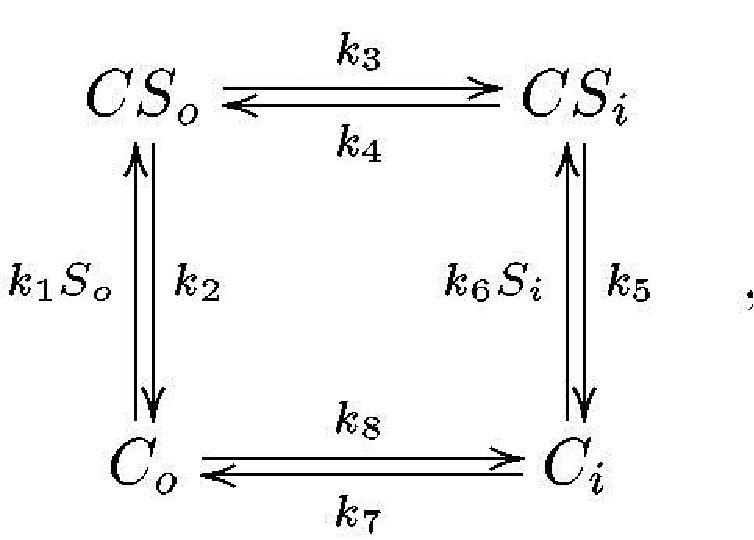
\includegraphics[width=7cm]{figures/fig_621.pdf}
	\caption{Схема переноса. $C$ --- переносчик, $S$ --- субстрат.}
	\label{fig.621}
\end{figure}

Начальная скорость переноса вещества (субстрата) определяется уравнением, аналогичным уравнению Михаэлис-Ментен:
\begin{equation}
	J = \frac{J_{max}S_0}{K_m+S_0},
\end{equation}
где $S_0$ --- концентрация субстрата по внешнюю сторону мембраны,\\
$K_m$ --- концентрация субстрата, при которой $J=\frac{J_{max}}{2}$.

Движущей силой транспорта с участием переносчика является градиент химического или электрохимического потенциала вещества. Функционирование систем с облегченной диффузией, так же как и простой диффузии, направлено на выравнивание градиентов и установление равновесия в системе. Однако градиенты вещества могут поддерживаться длительное время за счет того, что проникающие молекулы потребляются или образуются в ходе биохимических реакций по одну из сторон мембраны. 

Ткани животных обладают системами облегченной диффузии для ряда метаболитов, которые они получает из плазмы крови, например для сахаров, аминокислот, пуринов и глицерина.

\subsection{Транспорт ионов}

Существует несколько возможных механизмов прохождения ионов через мембрану: 
\begin{enumerate}
\item растворение иона в липидной фазе мембраны, диффузия и последующий переход из мембраны в раствор; 
\item движение по ионным каналам, являющимся структурными компонентами мембран; 
\item транспорт с участием переносчиков. 
\end{enumerate}

Эти механизмы переноса установлены как для биологических мембран, так и для бислойных липидных мембран. Отдельную категорию составляет транспорт через мембранные барьеры клетки по механизму пиноцитоза. Скорость проникновения ионов через мембрану определяется такими ее свойствами, как толщина, значение диэлектрической проницаемости, наличие фиксированных электрических зарядов на ее поверхности, знак и плотность расположения этих фиксированных зарядов на мембране, размеры и число пор в мембране, наличие фиксированных зарядов в порах, и некоторыми другими. 

Пассивное движение ионов происходит из области с высоким электрохимическим потенциалом в область с более низким электрохимическим потенциалом. Движущей силой переноса ионов является градиент электрохимического потенциала, обуславливающий в свою очередь разность химических потенциалов данного вещества в двух областях, между которыми происходит диффузия.

Взаимодействие иона с молекулами растворителя определяет значение стандартного химического потенциала $\mu_0$. В воде гидратация ионов приводит к изменению их эффективного радиуса. Радиус гидратированных ионов обычно оценивают с помощью соотношения Стокса-Эйнштейна:
\begin{equation}
	r = \frac{kT}{6\pi D\eta},
\end{equation}
где $D$ --- коэффициент диффузии,\\
$\eta$ --- вязкость среды.

Дегидратация любого иона щелочных металлов является энергетически невыгодной. Энергия гидратации равна энергии поляризации диэлектрика сильным локальным полем иона. Чем выше значение диэлектрической проницаемости среды, тем сильнее поляризация и более стабилен ион.

Согласно электростатической теории Борна, энергия иона радиусом $r$ в среде с диэлектрической проницаемостью определяется формулой:
\begin{equation}
	W = \frac{Z^2e^2}{8\pi r \varepsilon \varepsilon_0},
\end{equation}
а приращение свободной энергии при прохождении границы раздела сред в расчете на моль ионов 
\begin{equation}
	\Delta W = \frac{Z^2e^2N}{8\pi \varepsilon_0 r} \left( \frac{1}{\varepsilon_2} -
		\frac{1}{\varepsilon_1} \right).
\end{equation}

\subsection{Ионное равновесие на границе раздела фаз}

Ионное равновесие между двумя водными растворами, разделенными мембраной, описывается наиболее просто. В случае равновесия по ионам одного типа электрохимические потенциалы иона в обоих растворах одинаковы:
\begin{equation}
	RT \ln C_1 + zF \varphi_1 = RT \ln C_2+zF \varphi_2,
\end{equation}

откуда 
\begin{equation}
	\Delta \varphi = \varphi_2 - \varphi_1 = \frac{RT}{zF} \ln\frac{C_1}{C_2}.
\end{equation}
 
Уравнение Нернста показывает, что в условиях электрохимического равновесия разность потенциалов на мембране определяется соотношением концентраций данного иона в двух соприкасающихся растворах. После перехода к десятичным логарифмам и подстановке $2,3RT/F$ и 58 мВ (при температуре $20^o C$) уравнение Нернста для одновалентных ионов принимает вид: 
\begin{equation}
	\Delta \varphi=58 \lg\frac{C_1}{C_2}
\end{equation}

В биологических системах распределение $K^+$ между цитоплазмой животных клеток и средой достаточно хорошо соответствует уравнению Нернста. Однако распределение $Na^+$ в большинстве клеток резко отличается от равновесного. Рассмотрим ионное равновесие на границе вода-неполярный растворитель. Такая система может рассматриваться как модель границы раздела вода-липидная мембрана с диэлектрической проницаемостью 2---3. Представим систему из двух несмешивающихся жидкостей, например масло-вода, в которой растворен электролит $A^+B^-$. Вследствие неодинаковой липофильности ионов $A^+$ и $B^-$ между объемами фаз возникает так называемая межфазная разность потенциалов. 

На границе раздела потенциал и концентрации ионов испытывают скачки:

\begin{figure}[ht] \center
\label{fig.622}
	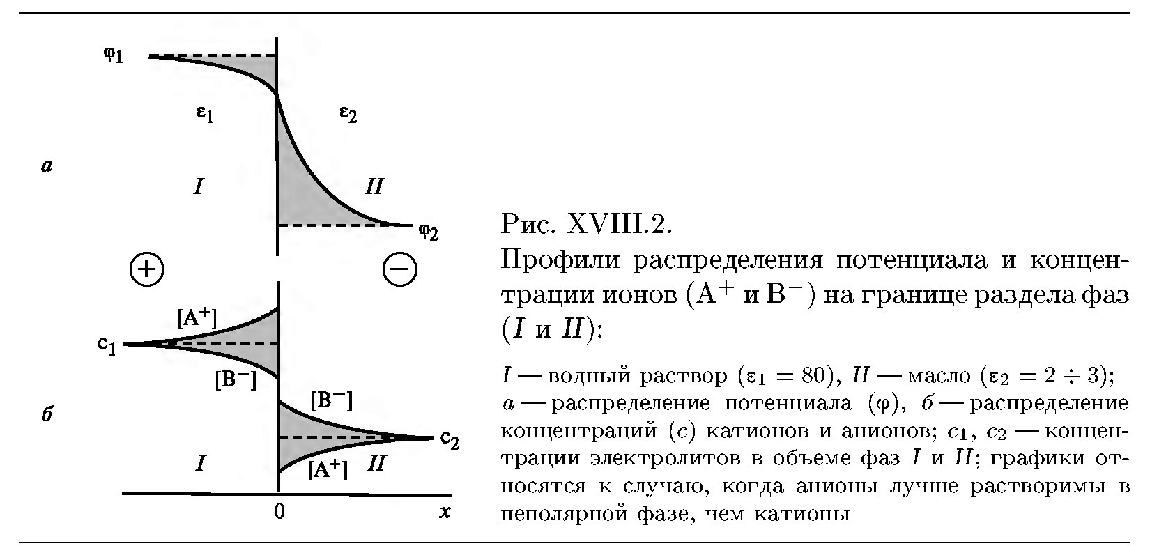
\includegraphics[width=10cm]{figures/fig_622.pdf}
	\caption{Профили распределения иотенциала и концентрации ионов ($A^+$ и $B^-$) на границе раздела фаз ($I$ и $II$)}
\end{figure}

\par\bigskip {\bf Электрохимическое уравнение Нернста-Планка}

В электродиффузионной модели мембрану рассматривают как непрерывную гомогенную среду, в которой происходит диффузия точечных невзаимодействующих частиц. Суммарный поток произвольного вида ионов $j$, движущихся пассивно и независимо в такой гомогенной среде в направлении оси $x$, пропорционален концентрации ионов, их подвижности и действующей на ион силе. Общее транспортное уравнение имеет вид: 
\begin{equation}
	\text{поток} = \text{концентрация} \times \text{действующая сила} \times \text{подвижность}.
\end{equation}

Таким образом, поток $J$ ионов $j$, концентрация которых в плоскости $x$ равна $C$, а подвижность $u$, равен
\begin{equation}
	J = Cu \left( - \frac{d\overset{-}{\mu}}{dx} \right).
\end{equation}
 
Учитывая определение электрохимического потенциала
\begin{equation}
	\overset{-}{\mu}=\mu_0+RT \ln C+zF\varphi,
\end{equation}

и с учетом
\begin{equation}
	\frac{d\ln C}{dx}=\frac{1}{C} \frac{dC}{dx},
\end{equation}
 
получим 
\begin{equation}
	\label{621}
	J = -uRT \frac{dC}{dx} - uCzF \frac{d \varphi}{dx}.
\end{equation}
 
Уравнение (\ref{621}) называется уравнением электродиффузии или {\bf уравнением Нернста-Планка} и описывает диффузию ионов в растворе или в гомогенной незаряженной мембране. Первый член в правой части уравнения описывает свободную диффузию (диффузионная компонента общего потока), второй выражает миграцию ионов в электрическом поле (миграционная компонента).
 
Задача описания диффузии заряженных частиц предполагает решение системы двух уравнений, одно из которых --- уравнение Нернста-Планка, второе --- уравнение Пуассона. Для упрощения электро-диффузионной задачи вводят дополнительные условия, например допущение о постоянстве одного из градиентов в мембране $dC/dx=const$ или $d \varphi/dx$, или допущение об электронейтральности мембраны. 

В подходе Планка-Гендерсона к решению электродиффузионного уравнения предполагают, что условие электронейтральности выполняется не только для объема фаз, разделенных мембраной, но и для самой мембраны. Иначе говоря, предполагают, что концентрации катионов и анионов в любой плоскости по оси $x$ одинаковы $(C^+ = C^-)$. В стационарном состоянии при условии разомкнутой цепи суммарный электрический ток через мембрану не течет, т. е. сумма переносимых катионов равна сумме переносимых анионов. Для бинарного электролита, содержащего одновалентный катион и одновалентный анион, условие равенства потоков имеет вид:
\begin{equation}
	u_+RT \frac{dC}{dx}-u_+CzF \frac{d \varphi}{dx} = 
		u_-RT \frac{dC}{dx}-u_-CzF \frac{d \varphi}{dx}
\end{equation}
где $u$ с соответствующим знаком обозначает подвижность катиона или аниона в мембране
\begin{equation}
	\frac{d \varphi}{dx} = \varphi_2-\varphi_1 = 
		-\frac{u_+-u_-}{u_++u_-} \frac{RT}{F} \frac{1}{C}\frac{dC}{dx}
\end{equation}

\begin{equation}
	\label{622}
	\Delta \varphi = -\frac{u_+-u_-}{u_++u_-} \frac{RT}{F} \ln \frac{dC}{dx}
\end{equation}

Уравнение (\ref{622}) называется {\bf уравнениемем Гендерсона} и иллюстрирует принцип Ле-Шателье, т.к. при смешении растворов разной концентрации и их взаимопроникновении через перегородку потенциал определенного знака, создаваемый ионом того же знака, имеющим большую подвижность, будет <<привлекать>> ионы противоположного знака и скорости диффузии ионов обоих знаков, т.о., выровняются. Уравнение Гендерсона несправедливо в случае липидных и клеточных мембран, для которых условие локальной электронейтральности не выполняется (липофильность катионов и анионов разная, поэтому разные концентрации их в мембране). 

В случае тонких биологических (клеточных) мембран применяется другой, несколько более сложный, дискретный подход к решению уравнения Нернста-Планка. Основан он на том факте, что при прохождении по каналу ионы перескакивают из одной пот.ямы в другую.

\par\bigskip {\bf Индуцированный транспорт ионов}

Основные закономерности транспорта ионов через мембраны изучены в опытах с различными моделями, из которых самой близкой к биомембранам оказалась {\it бислойная липидная мембрана (БЛМ)}. 

Затраты энергии, необходимые для проникновения иона в неполярную фазу, можно оценить по формуле Борна, согласно которой энергия, затрачиваемая на перемещение иона из воды в мембрану, зависит от его радиуса $r$ и диэлектрических проницаемостей воды $\varepsilon_w$ и мембраны $\varepsilon_m$. 

В системе СГС: 
\begin{equation}
	W = \frac{Z^2e^2}{2r} \left( \frac{1}{\varepsilon_m} -
		\frac{1}{\varepsilon_{w}} \right).
\end{equation}

Рассчитанные по данному уравнению значения свободной энергии для перехода $Na^+$ и $K^+$ из воды в неполярный растворитель $\varepsilon_m = 2$ составляют большую величину 250-350 кДж/моль. Именно это создает барьер, препятствующий прохождению ионов щелочных металлов через гидрофобную часть липидного бислоя в негидратированной форме. 

Как видно из формулы выше, энергия перехода иона в мембрану снижается с увеличением радиуса иона. Поэтому крупные органические ионы проникают через БЛМ легче, чем катионы щелочных металлов. Для таких крупных липофильных ионов, как дипикриламин и тетрафенилбор, возможно прямое прохождение через мембрану. При изменении градиента концентрации в случае одного проникающего иона разность электрических потенциалов на БЛМ изменяется в соответствии с уравнением Нернста. Этим методом было продемонстрировано пассивное движение проникающих ионов через мембраны митохондий, субмитохондриальных частиц, бактериальных хроматофоров при энергозависимой генерации мембранного потенциала. 
Как видно из величина энергетического барьера в мембране уменьшается, а следовательно, проницаемость мембраны для иона возрастает не только при увеличении его радиуса, но и при приближении значений $\varepsilon_m$ к $\varepsilon_w$. На этих физических принципах и основан перенос ионов ионофорами. Ионофоры могут образовывать с ионом комплекс большого размера --- переносчики --- либо формировать пору в мембране, заполненную водой, --- каналы. Это механизмы переноса --- с участием переносчиков и через ионные каналы --- изучены наиболее подробно в опытах с БЛМ.

\begin{figure}[ht] \center
	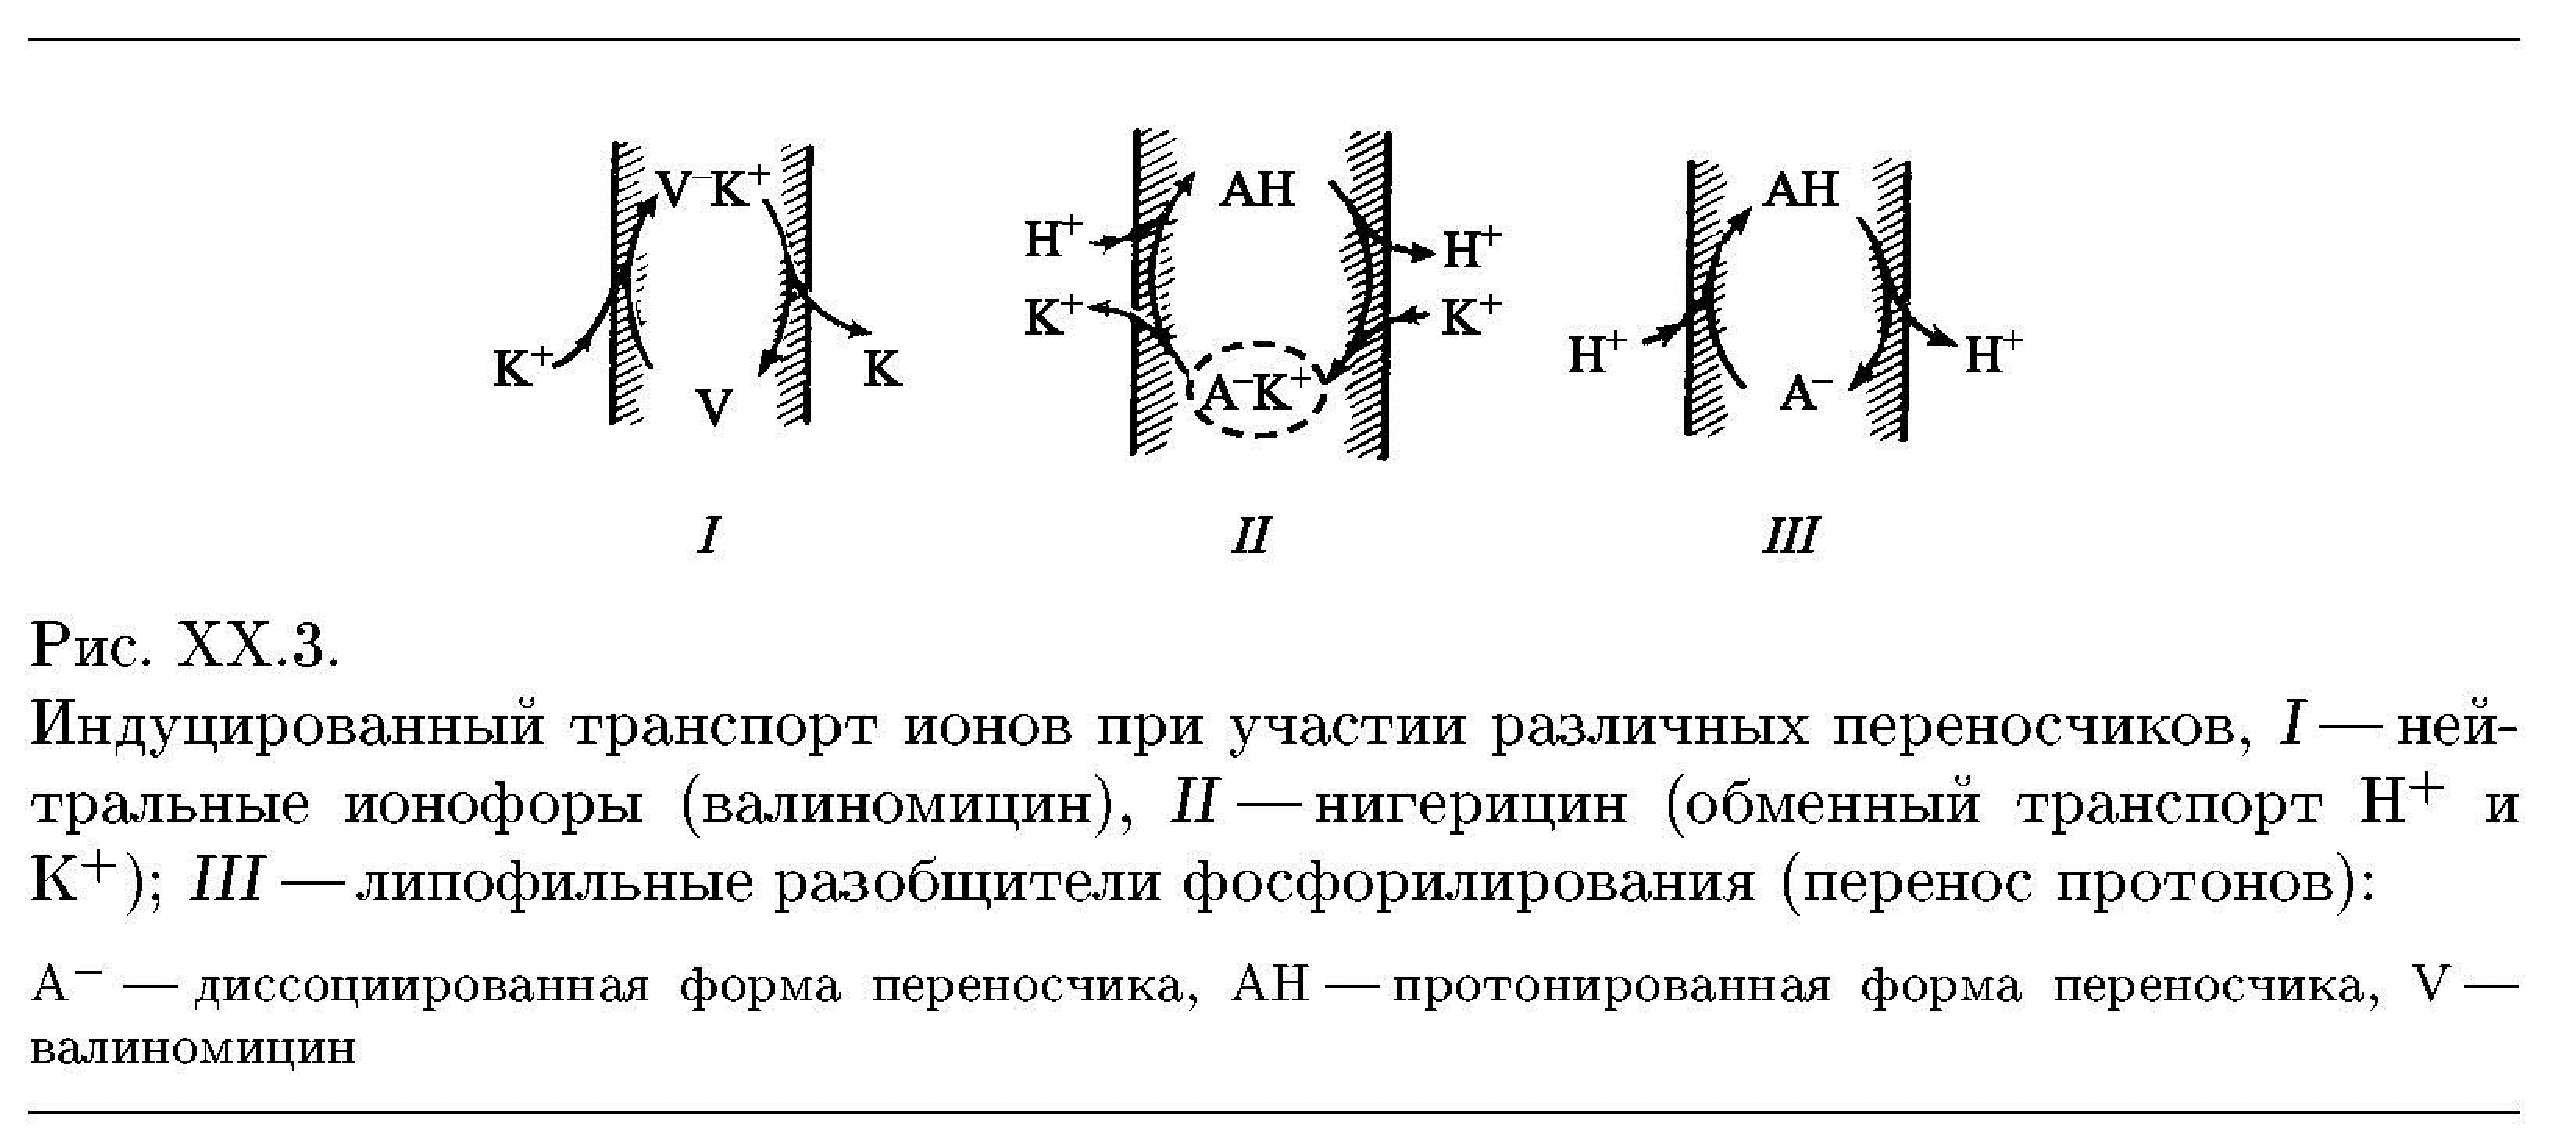
\includegraphics[width=10cm]{figures/fig_623.pdf}
	\caption{Индуцированный транспорт ионов при участии различных переносчиков}
	\label{fig.623}
\end{figure}

На рисунке I --- нейтральные ионофоры (валномицин), II --- нигерицин (обменный транспорт $H^+$ и $K^+$); III --- липофильные разобщители фосфорилирования (перенос протонов): {\small $A^-$ --- диссоциированная форма переносчика, $AH$ --- протонированная форма переносчика, $V$ --- валиномицин}

Перенос иона через мембрану с участием переносчика включает стадии образования комплекса иона с ионофором на одной стороне мембраны, перемещения комплекса через мембрану, освобождения иона на другой стороне и возвращения ионофора. Возможны две схемы работы переносчика: малая <<карусель>>, когда ионофор не выходит из мембраны, и большая <<карусель>>, когда ионофор проходит мембрану насквозь, а образование и распад комплексов протекает в неперемешиваемых слоях около мембраны. По механизму малой карусели около мембраны. По механизму малой карусели осуществляется, например, перенос $K^+$ в присутствии валиномицина. 
Энергия комплекса ион-переносчик оказывается значительно меньше энергии дегидратированного иона. Так, для заряженного комплекса радиусом 1 нм свободная энергия перехода из воды в мембрану составляет около 15 кДж/моль в отличие от значений 250-350 кДж/моль, соответствующих энергии дегидратации свободных ионов с радиусом 0,1---0,15 нм. 
Среди соединений, относящихся к ионным переносчикам, центральное место занимают макроциклические антибиотики, выделенные из микроорганизмов, и ряд синтетических макроциклических комплексонов.
Некоторые соединения из этой группы --- нейтральные ионофоры --- не содержат ионизируемых групп. Это циклические полипептиды, циклические молекулы, состоящие из чередующихся аминокислот и $\alpha$-оксикислот (так называемые депсипептиды, примером которых являются валиномицин и его аналоги), макроциклические структуры, включающие четыре лактоновых кольца, --- макротетролиды (нонактин) --- и некоторые синтетические циклические полиэфиры. Комплексы, образуемые нейтральными макроциклическими соединениями с ионами щелочных металлов, несут положительный заряд. Перенос иона через мембрану происходит в виде заряженного комплекса.

Движение иона значительно облегчается, если молекулы ионофора образуют комплекс, имеющий водную пору --- канал. Наиболее известными каналообразующими соединениями являются грамицидин $A$, аламетицин, амфотерицин, мицин и полиеновые антибиотики.
Все эти молекулы обладают сродством к водной и органической фазам, что, с одной стороны, позволяет им образовывать водную пору, а с другой --- приводит к сильной сорбции антибиотика на мембрану. Внешняя часть молекул в поре гидрофобна, а внутрь канала обращены хорошо поляризуемые группы. Заряженные или сильно полярные группы могут находиться на одном конце молекулы. Такие группы служат <<якорем>>, удерживая полярный конец на одной из сторон мембраны, позволяя молекуле пронизать гидрофобную часть мембраны.


\newpage
%%%%%%%%%%%%%%%%%%%%%%%%%%%%%%%%%%%%%%%%%%%%%%%%%%%%%%%%%%%%%%%%%%%%%%%%%%%%%%%%%%%%%%%%
\section{Активный транспорт}
{\it Молекулярное строение каналов. Каналы и транспорт ионов через них. Электронейтральный и электрогенный транспорт ионов. Калий-натриевый насос. Активный транспорт кальция. Транспорт протонов. Активный транспорт нейтральных молекул.}

{\bf Активный транспорт} --- это перенос вещества через клеточную или внутриклеточную мембрану (трансмембранный активный транспорт) или через слой клеток (трансцеллюлярный активный транспорт), протекающий против электрохимического градиента, т. е. с затратой свободной энергии организма. 

В большинстве случаев источником энергии служит энергия макроэргических связей АТФ. Различные транспортные АТФазы, локализованные в клеточных мембранах и участвующие в механизмах переноса веществ, являются основным элементом молекулярных устройств --- насосов, обеспечивающих избирательное поглощение и откачивание определенных веществ клеткой, например электролитов. Активный специфический транспорт неэлектролитов (молекулярный транспорт) реализуется с помощью нескольких типов молекулярных машин --- насосов, переносчиков, каналов и пр. Транспорт неэлектролитов (моносахаридов, аминокислот и других мономеров) может сопрягаться с механизмом транспорта другого вещества, движение которого по градиенту концентраций является источником энергии для первого процесса. Вторичная энергизация может обеспечиваться ионными градиентами (например, натрия) без непосредственного участия АТФ, а также некоторыми другими механизмами, природа которых не ясна (например, натрийзависимый транспорт мономеров, освобождающихся при мембранном гидролизе ди- и олигомеров).

\subsection{Молекулярное строение каналов}

Известно, что для выявления механизмов активации и инактивации каналов, их селективности, блокировки, прохождения ионов через пору и других функциональных свойств необходимо знание структуры макромолекул, входящих в состав канала.

В середине 70-х гг. было установлено, что $K^+$--канал ($4,5 \times 4,5 \text{\AA}$) представляет собой трансмембранный белок, погруженный в липидный бислой. Аналогичный вывод был получен и в отношении другого типа каналов, изменение проводимости которых достигается не за счет изменения электрического потенциала на мембране, а в результате действия химических нейромедиаторов.

Методы генной инженерии позволили детально раскрыть структуру белков $Na^+$-- ($3.1 \times 5.1 \text{\AA}$), $K^+$--, $Ca^{2+}$--каналов. Установлено, что основным носителем функциональных свойств в натриевых и кальциевых каналах являются большие $\alpha$-- (в натриевом канале) и $\alpha_2$-- (в кальциевом канале) субъединицы, состоящие из четырех повторов по 300--400 аминокислот в каждом. В свою очередь, каждый из этих повторов включает в себя 6 трансмембранных $\alpha$--спиральных сегментов ($S_1$, $S_2$, $S_3$, $S_4$, $S_5$, $S_6$).

Особая роль среди них в обеспечении функциональных свойств канала принадлежит сегменту $S_4$, который несет положительные заряды от 4 до 8 на каждом третьем остатке аргинина или лизина. 

Этот сегмент $S_4$, возможно, играет роль сенсора в воротном механизме канала. В натриевых и кальциевых каналах одна большая субъединица достаточна для обеспечения работы канала.

 
\subsection{Каналы и транспорт ионов через них}

При продвижении иона по узкому однорядному каналу возможно взаимодействие ионов друг с другом и с молекулярными группами канала. При поступлении иона в канал происходит замещение гидратной оболочки иона полярными группами канала. Увеличение свободной энергии иона при дегидратации с лихвой компенсируется энергией его взаимодействия с полярными группами канала, в результате чего его свободная энергия понижается и прохождение по каналу облегчается. Наличие полярных групп и фиксированных анионных центров в канале приводит за счет их кулоновского взаимодействия с ионом к снижению энергетического барьера перехода иона из раствора в канал. Лучше всего проходят через канал ионы, прочно связывающиеся кулоновским взаимодействием с анионным центром. После потери гидратной оболочки меньший по размеру ион натрия лучше связывается с анионным центром, чем ион калия. В качестве анионного центра натриевого канала могут выступать атомы кислорода группы $COO^-$. Через натриевые каналы могут проходить также органические ионы размером не более 3 $\times$ 5 $\overset{\circ}{A}$. Калиевые каналы имеют широкое (более 8 $\overset{\circ}{A}$) устье со стороны цитоплазмы. 

Однорядный транспорт характеризуется тем, что каждый следующий ион не может попасть в занятую другим ионом потенциальную яму из-за кулоновского отталкивания между ионами. Перескоки между ямами совершаются под действием тепловых флуктуаций. Проводимость канала зависит от того, насколько заполнены участки <<входа>> и <<выхода>> канала, связывающие ионы (чем больше заполнение, тем ниже проводимость). Выход из канала иона, связанного анионным центром, облегчается при появлении на входе канала другого иона вследствие их ион-ионного кулоновского отталкивания.

\begin{figure}[ht] \center
\label{fig.631}
	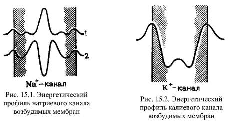
\includegraphics[width=10cm]{figures/fig_631.pdf}
	\caption{Индуцированный транспорт ионов при участии различных переносчиков}
\end{figure}

\subsection{Электронейтральный и электрогенный транспорт ионов}

{\bf Электронейтральный транспорт ионов} --- такой транспорт, при котором функционирование транспортной системы сопровождается обменом внутриклеточных ионов в соотношении <<заряд на заряд>>. Система активного транспорта является лишь средством поддержания концентрационных градиентов и не участвует непосредственно в создании разности потенциалов на клеточной мембране. Потенциал на мембране создается только за счет диффузии ионов по градиентам концентрации. 

Если число зарядов, переносимых в одном направлении в единицу времени, не компенсируется суммой зарядов, переносимых в другом направлении, транспортный механизм непосредственно участвует в создании дополнительной разности потенциалов на мембране --- {\it электрогенный режим} (3 натрия на 2 калия --- $Na$--$K$ насос).


\subsection{Калий-натриевый насос}

Калий-натриевый насос --- мембранный механизм, поддерживающий определённое соотношение ионов $Na^+$ и $K^+$ в клетке путём их активного транспорта против электрохимического и концентрационного градиентов.

Клетки большинства тканей содержат больше ионов $K^+$, чем $Na^+$, в то время как в омывающей их жидкости (кровь, лимфа, межклеточная жидкость) значительно выше концентрация $Na^+$. Определённое количество ионов постоянно входит в клетки и покидает их. 

Пассивный транспорт катионов (движение ионов через мембрану по системе специальных каналов вдоль электрохимического и концентрационного градиентов) в норме компенсируется активным транспортом ионов. Функционирование насоса связано с переносом метаболитов в клетки, а для нервных и мышечных волокон также с механизмом возбуждения. Работа насоса в целом зависит от интенсивности метаболизма клетки и сопровождается накоплением на мембране разности электрических потенциалов.

Этот процесс сопровождается расщеплением АТФ, т.е.является эндоэргическим. Насос представляет собой не что иное, как фермент, расщепляющий АТФ,--- натрий--калий--зависимую АТФ--азу. Этот фермент обычно расположен в мембранах и активируется при повышении концентрации ионов натрия внутри клетки или ионов калия в наружной среде. Большинство исследователей склоняется к мысли, что насос действует по принципу открывающихся и закрывающихся каналов. Предполагается, что натриевые и калиевые каналы соседствуют друг с другом. Связывание молекул <<канального>> белка с ионом натрия приводит к нарушению вторичной структуры белка, в результате чего меняется его конформация. Обычная $\alpha$--спираль, в которой на каждый виток приходится 3,6 аминокислотного остатка, переходит в более рыхлую $\beta$--спираль (4,4 аминокислотного остатка). В результате образуется внутренняя полость, достаточная для прохождения иона $Na^+$, но слишком узкая для иона калия. После прохождения $Na^+$ $\beta$--спираль переходит в туго свернутую так называемую спираль 310 (это означает, что 3 аминокислотных остатка приходится на виток и водородная связь у каждого десятого атома). При этом натриевый канал закрывается, а стенки соседнего калиевого канала раздвигаются, образуя полость, достаточно широкую для прохождения иона калия. Натрий--калиевый насос работает по принципу перистальтического насоса (наподобие передвижения пищевого комка по кишечнику).


\subsection{Активный транспорт кальция}

Кальций-зависимая АТФаза, сопряженная с мощным кальций-насосом, локализована в мембранах саркоплазматической сети и имеет некоторые сходные черты с натрий калиевой АТФазой. $Ca$ --АТФаза состоит из одной полипептидной цепи с молекулярной массой около 100 кДа и относительно высоким содержанием гидрофобных аминокислот. Для работы кальций-зависимой АТФазы также необходимо присутствие фосфолипидов.

Работу $Ca$--АТФазы изучают на фрагментах саркоплазматическото ретикулума, выделяемых из мышечной ткани, а также на мембранных пузырьках, которые образуются в определенных условиях в смеси очищенного препарата $Ca$--АТФазы с фосфолипидами. Схема работы $Ca$--АТФазы может быть представлена следующим образом. На первом этапе происходит связывание $Ca$ и АТФ. Эти соединения связываются с разными центрами на внешней поверхности мембранного пузырька. Константа связывания $Ca$ составляет порядка 107 $M^{-1}$. На втором этапе АТФ гидролизуется с образованием фосфорилированного фермента. Образование фермент-фосфатного комплекса можно обнаружить по включению в белок радиоактивного изотопа $32P$ из АТФ, меченной по фосфату. Образующаяся фосфорилированная форма фермента $E \sim P$ конформационно неустойчива и претерпевает изменение пространственной структуры так, что ион-связывающие участки оказываются отделенными от внешней среды. 

На следующем этапе цикла происходит изменение сродства $Ca$--связывающих центров к ионам $Ca$ одновременно с изменением характера связи фосфатной груп- группы с ферментом. Энергия, ранее сосредоточенная в макроэргической фосфатной связи комплекса $E \sim P$ , расходуется на изменение константы связывания ионов $Ca$ с ферментом. Как и в случае $Na^+$, $K^+$--АТФазы, изменение сродства обусловлено, по-видимому, изменением расположения полярных групп, образующих координационные связи с $Ca^{2+}$. Вследствие происшедшего изменения пространственной структуры фермента ионы $Ca$ получают доступ во внутреннее пространство мембранных пузырьков и выбрасываются во внутренний объем. Константа связывания $Ca$ при образовании стабильной фосфорилированной формы фермента уменьшается.

На основании соотношения, связывающего константу химического равновесия с изменением свободной энергии в ходе реакции $\Delta G_0$, т. е. $\Delta G_0 = -RT \ln K$, можно найти, что изменение свободной энергии при уменьшении константы связывания составляет 17,8 кДж/моль. Таким образом, суммарные затраты энергии на перенос $Ca$ через мембрану примерно вдвое меньше энергии гидролиза АТФ (около 40 кДж/моль при $pH$=9), которой хватает на перенос двух ионов $Ca^{2+}$. Вследствие десорбции $Ca^{2+}$ с фермента суммарный положительный заряд в ион-связывающей полости уменьшается, что значительно облегчает десорбцию фосфата. В результате этих превращений фермент вновь приходит в исходное состояние.

\subsection{Транспорт протонов}

Перенос электронов в энергосопрягающих мембранах митохондрий, хлоропластов и бактерий сопровождается трансмембранным переносом $H^+$ и образованием градиента электрохимического потенциала этого иона $\Delta \mu_{H^+}$, который включает электрический (мембранный потенциал) и концентрационный (градиент $pH$) компоненты: 

\begin{equation}
\label{631}
\Delta \overset{-}{\mu}_H=RT \ln \left( \frac{C_1}{C_2} \right)+zF(\varphi_i- \varphi_0 )=zF \Delta \varphi-2,3RT \Delta pH
\end{equation}
 
В выражении (\ref{631}) индексы $i$ и $0$ относятся к растворам, находящимся внутри и снаружи замкнутой мембранной системы. В сопрягающих мембранах локализованы также АТФ--синтетазные системы, через каналы которых осуществляется пассивное движение $H^+$ по градиенту электрохимического потенциала.

Перенос $H^+$ через мембраны может осуществляться механизмами трех типов: 

\begin{enumerate}
\item В некоторых мембранах существуют подвижные переносчики протонов (пластохинон в фотосинтетической мембране хлоропластов). 
\item Возможны также конформационные переходы мембранного белка при связывании протона на одной стороне мембраны и депротонировании белка с другой стороны мембраны. 
\item Протоны могут транспортироваться через мембрану по специализированным структурам --- $H^+$--каналам. 
\end{enumerate}

Протонный канал представляет собой узкую полость, образованную полярными группами белка. Протонный канал --- важный компонент всех $H^+$--АТФаз. Он образован гидро-- гидрофобной частью субъединицы сопрягающего фактора --- комплексом $CF_0$. По $H^+$-- каналу протоны поступают к каталитическому участку транспортной системы, в котором осуществляется сопряжение переноса $H^+$ с реакциями синтеза-гидролиза АТФ. Таким образом, основными узлами $H^+$--насосов являются протонный канал и активный центр.

Транспорт протонов по $H^+$--каналам обычно сравнивают с переносом $H^+$ по регулярной решетке, образованной системой водородных связей, аналогичной таковой во льду. В структуре льда возможны переходы протона от одной молекулы воды к соседней. В результате возникает ионная пара, состоящая из положительно заряженного иона гидроксония $H_3O^+$ и гидроксила $OH^-$. В отсутствие электрического поля обмен протонами происходит хаотично, однако при создании разности потенциалов возникает направленная миграция дефектов. В итоге достигается быстрое смещение протонов вдоль упорядоченной цепи водородных связей.

В биологических мембранах системы водородных связей, по которым транспортируются протоны, образованы полярными группами, не участвующими в формировании $H$--связей $\alpha$--спирали полипептидной цепи. Для формирования сквозной трансмембранной структуры, транспортирующей $H^+$, необходимо около 20 аминокислотных остатков.

В общем виде систему активного транспорта рассматривают как трансмембранный канал с большим числом участков связывания $H^+$, в котором транслокация протонов происходит за счет последовательных перескоков Н+ между участками связывания. Такой ионный канал может работать как ионный насос, если структура энергетических барьеров претерпевает динамические изменения за счет энергообеспечивающей реакции, например изменяются константа диссоциации протон связывающих участков канала и высота соседних барьеров. В этом случае протон будет освобождаться преимущественно с одной стороны мембраны, а поглощаться --- с другой. 

Изменение высоты активационных барьеров, обусловленное небольшими изменениями конформации $H^+$ канала, может быть связано с изменением $pKa$ сродства к протону аминокислотных остатков переносчиков $H^+$. Рассмотренная схема может быть распространена на $H^+$--насосы, использующие в качестве источника энергии разность окислительно--восстановительных потенциалов. В этом случае разные конформационные состояния канала соответствуют окисленной и восстановленной форме ферментов --- переносчиков электрона. Аналогичным образом можно описать АТФ--зависимый транспорт протонов.

\subsection{Активный транспорт нейтральных молекул}

...


\newpage
%%%%%%%%%%%%%%%%%%%%%%%%%%%%%%%%%%%%%%%%%%%%%%%%%%%%%%%%%%%%%%%%%%%%%%%%%%%%%%%%%%%%%%%%
\section{Способность к молекулярной рецепции --- необходимое условие функционирования биологических систем}
{\it Понятие молекулярной рецепции. <<Сквозное>> присутствие молекулярной рецепции практически во всех биологических реакциях. Молекулярная рецепция в функционировании ферментов. Каскады ферментативных реакций. }

\subsection{Понятие молекулярной рецепции}

Специфичность --- и есть свойство ферментов. Рецепция лежит в основе живого.

Узнавание (распознавание) сигнала рецептором есть основное свойство регулируемой и регулирующей системы, осуществляющей классификацию объектов, воздействующих на рецепторы.

Распознающие системы могут быть 1) необучающимися и 2) обучающимися.

Клеточное распознавание имеет принципиальное значение для процессов развития, в частности, для возникновения иммунитета. Молекулярное распознавание (рецепция) определяет все важнейшие молекулярно-биологические процессы --- ферментативную активность, редупликацию ДНК, все этапы биосинтеза белка, взаимодействие антиген-антитело, и т.д.

Молекула белка-фермента узнает молекулу субстрата или некоторую ее часть, как, например, в случае протеолитических ферментов, катализирующих гидролиз пептидных связей. Рецепция выражается в образовании реакционного комплекса со специфическим субстратом. Комплексы с ингибиторами и активаторами, с аллостерическими эффекторами также возникают в результате специфического узнавания.

Еще пример: узнавание гидрофобных остатков гидрофобными же остатками, вследствие чего формируется ядро глобулы.

Более простой случай рецепции: комплементарное связывании нуклеотидов в двойной спирали ДНК, в гибридной двойной спирали ДНК-РНК, при взаимодействии кодон-антикодон.

Приходим к термину <<молекулярная рецепция>>. Это понятие имеет смысл применительно к системам, в которых узнающее устройство сохраняет свою целостность в акте узнавания и в ряде случаев возвращается в исходное состояние, совершая преобразование молекулярного сигнала. Одна молекула фермента перерабатывает множество молекул субстрата, одна рибосома <<читает>> весь текст, записанный в цепи мРНК. В биосинтезе белка ферментативная рецепция происходит в акте транскрипции, в котором участвуют РНК-полимераза, и в акте трансляции, где узнающими системами, наряду с мРНК, служат аминоацил-тРНК синтетаза, вся рибосома и пр.

Таким образом, определение молекулярной рецепции указывает на специфичность слабых, главным образом нехимических взаимодействий молекул. {\bf Для узнавания существенно стерическое соответствие структуры рецептора и сигнатуры сигнальной молекулы, соответствие, фиксированное или индуцируемое. Специфическое понижение свободной энергии происходит вследствие многоточечного взаимодействия, которое и описывается как континуальное соответствие молекулярных поверхностей и находит свое наглядное выражение в атомных моделях.}

{\bf Молекулярное кодирование в биологии основывается в конечном счете на молекулярной рецепции.} Генетический код связан с функционированием ряда узнающих систем, перечисленных выше. Естественно возникает вопрос о ферментном коде, т.е. о классификации соответствий между активными центрами ферментов и субстратов. Громадное число комбинаций из 20 сортов аминокислотных остатков на поверхности реактивной полости фермента, в его активном центре, обеспечивает неограниченное многообразие функциональности ферментов. Можно думать о наличии фиксированных комбинаций, кодирующих узнавание характерных атомных групп субстратов. Точнее следует говорить о кодовых сорбирующих комбинациях и кодовых каталитических комбинациях, действующих согласованно, но пространственно разделенных.

Взаимодействие, определяющее узнавание субстрата или ингибитора белком, есть процесс передачи информации молекулярным сигналом рецептору. По Кастлеру, {\bf в большинстве реальных случаев передается не вся информация, содержащаяся в данном объекте, но лишь некоторая ее часть, именуемая сигнатурой. Сигнатурой молекулы служат все те ее особенности, благодаря которым она становится участником данной реакции.} В случае образования фермент-субстратного комплекса сигнатурой субстрата являются его функциональные группы, взаимодействующие с активным центром. В свою очередь, сигнатура фермента есть его активный центр, т.е. ограниченная совокупность аминокислотных остатков, непосредственно взаимодействующих с субстратом. Узнавание сводится здесь к структурному соответствию молекулярных сигнатур, реализуемому в результате многоточечных слабых взаимодействий.

Специфичность ферментов не абсолютна. Данный фермент зачастую катализирует не определенную реакцию одного строго заданного субстрата, а однотипные реакции группы сходных субстратов. Одна из причин наличия конечного интервала специфичности имеет молекулярно-кинетический характер. Реальная молекулярная распознающая система, фермент, предназначена не только для узнавания молекулярного сигнала, но и для его достаточно быстрого преобразования. Степень специфичности узнавания, вообще говоря, зависти от степени связывания субстрата, т.е. выражается свободной энергией взаимодействия. Если выигрыш свободной энергии слишком велик, то прочность фермент-субстратного комплекса может быть настолько большой, что число оборотов фермента окажется чрезмерно низким. {\bf Необходимо оптимальное соотношение между точностью узнавания и скоростью преобразования.}

Доведение событий молекулярной рецепции, то есть события на уровне отдельных молекул, до уровня целого организма осуществляется ферментативными каскадами. Все каскады имеют характерную для них общую структуру Рис. \ref{fig.341}.

\begin{figure}[ht] \center
\label{fig.341}
	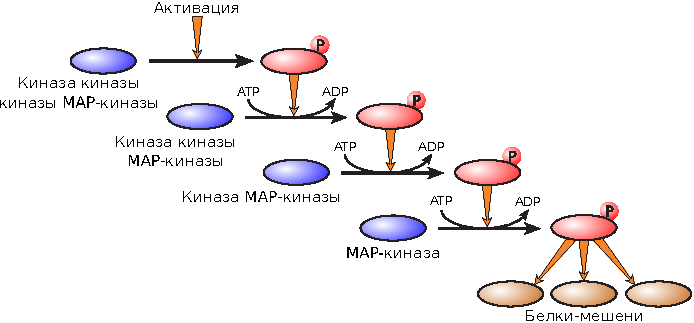
\includegraphics[width=10cm]{figures/fig_34_1.pdf}
	\caption{Общая схема каскадной сигнальной реакции \cite{Attuallahanov2000}}
\end{figure}

Пример --- действие адреналина. Роль <<тормоза>> выполняет фосфатаза, которая переводит активную форму киназы фосфорилазы в неактивную. При превышении пороговой концентрации адреналина фосфатаза ингибируется, каскад начинает развиваться и при этом ингибируется гликоген-синтаза, активность который мешает мобилизации энергетических ресурсов мышечной клетки.

Зачем нужны такие процессы в организме? Они могут выступать в качестве элементов конструктора из которых можно создавать устройства со сложной кинетикой. Например с помощью каскада легко сделать выключатель --- триггер, генератор импульсов определенной формы, или генератор колебаний. Боле того, недавно стало понятно, как с помощью каскадов природа может формировать сложные пространственные конструкции --- задача крайне важная в процессах пространственной дифференцировки многоклеточных организмов.

Общим свойством всех систем, использующих ферментативные каскады, является существование порога и ответ по типу все или ничего. Благодаря кинетическим свойствам каскада система, перевалив через порог, неудержимо и быстро устремляется к новому состоянию, характеристики которого практически не зависят от силы и кинетики воздействия, вызвавшего переход (рис. \ref{fig.342}).

\begin{figure}[ht] \center
\label{fig.342}
	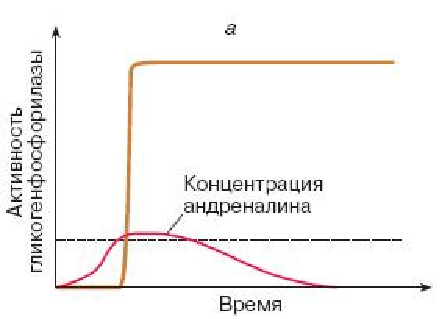
\includegraphics[width=6cm]{figures/fig_34_2.pdf}
	\caption{Кинетика адреналина}
\end{figure}

Другая особенность ферментативных каскадов состоит в том, что они не являются самостоятельными метаболическими или регуляторными системами. Они всегда являются частью системы, поведение которой зависит от устройства всей системы в целом. Это обеспечивает разнообразие возможных ответов.





( Почему бактерии --- сардельки, а не макароны? Потому-что они гетеротрофы и потребляют поверхностью. )


{\bf Механизмы координации внутриорганизменных химических и физиологических процессов.}

Нервная, гуморальная регуляция, генетическая, химические обратные связи.




\chapter{Физиология клетки}
%%%%%%%%%%%%%%%%%%%%%%%%%%%%%%%%%%%%%%%%%%%%%%%%%%%%%%%%%%%%%%%%%%%%%%%%%%%%%%%%%%%%%%%%
\section{Гомеостаз \\(клетки, ткани и организма)}

{\it Отрицательные и положительные обратные связи в организме. Элементы теории управления. Примеры проявления отрицательных обратных связей в организме. Принципы соорганизации процессов в клетке. Механизмы координации внутриорганизменных химических и физиологических процессов.}\\


Гомеостаз (греч. homoios --- подобный, тот же самый; stasis-состояние, неподвижность) --- относительное динамическое постоянство внутренней среды (крови, лимфы, тканевой жидкости) и устойчивость основных физиологических функций (кровообращения, дыхания, терморегуляции, обмена веществ и т.д.) организма человека и животных. Регуляторные механизмы, поддерживающие физиологическое состояние или свойства клеток, органов и систем целостного организма на оптимальном уровне, называются гомеостатическими. <<Сохранение структурно-функциональной стабильности>> --- суть любого гомеостаза, управляемого гомеостатом или саморегулируемого.

Как известно, живая клетка представляет подвижную, саморегулирующую систему. Ее внутренняя организация поддерживается активными процессами, направленными на ограничение, предупреждение или устранение сдвигов, вызываемых различными воздействиями из окружающей и внутренней среды. Способность возвращаться к исходному состоянию после отклонения от некоторого среднего уровня, вызванного тем или иным <<возмущающим>> фактором, является основным свойством клетки.

Как показывают исследования, существующие у живых организмов способы регуляции имеют много общих черт с регулирующими устройствами в неживых системах, таких как машины. И в том и в другом случае стабильность достигается благодаря определенной форме управления.

Особое значение для жизнедеятельности организма имеет постоянство состава крови. Хорошо известна устойчивость ее активной реакции (pH), осмотического давления, соотношения электролитов (натрия, кальция, хлора, магния, фосфора), содержания глюкозы, числа форменных элементов и т. д. Так, например, pH крови, как правило, не выходит за пределы 7,35-7,47. Наличие большого количества осморецепторов в тканях и органах и координированной системы регуляторов водного обмена и ионного состава позволяет организму быстро устранить сдвиги в осмотическом давлении крови, происходящие, например, при введении воды в организм.

Особо важное значение имеет постоянство внутренней среды для деятельности центральной нервной системы: даже незначительные химические и физико-химические сдвиги, возникающие в цереброспинальной жидкости, глии и околоклеточных пространствах, могут вызвать резкое нарушение течения жизненных процессов в отдельных нейронах или в их ансамблях. 

Особо важное значение имеет постоянство внутренней среды для деятельности центральной нервной системы: даже незначительные химические и физико-химические сдвиги, возникающие в цереброспинальной жидкости, глии и околоклеточных пространствах, могут вызвать резкое нарушение течения жизненных процессов в отдельных нейронах или в их ансамблях. 

К наиболее совершенным гомеостатическим механизмам в организме высших животных и человека относятся процессы терморегуляции; у гомойотермных животных колебания температуры во внутренних отделах тела при самых резких изменениях температуры в окружающей среде не превышают десятых долей градуса.

Организующая роль нервного аппарата лежит в основе широко известных представлений о сущности принципов гомеостаза. Примером решения проблемы гомеостаза с позиций кибернетики является попытка Эшби сконструировать саморегулирующее устройство, моделирующее способность живых организмов поддерживать уровень некоторых величин в физиологически допустимых границах.

Французский исследователь К. Бернар писал, что условием свободного поведения живого организма является постоянство внутренней среды. По его мнению, все жизненные процессы имеют одну цель --- поддержание постоянства условий жизни во внутренней среде организма. Позднее эта мысль нашла воплощение в трудах американского физиолога У. Кеннона в форме учения о гомеостазе.

Гомеостаз --- относительное динамическое постоянство внутренней среды и устойчивость физиологических функций организма. Основным механизмом поддержания гомеостаза является саморегуляция.

Саморегуляция --- вариант управления, при котором отклонение какой-либо физиологической функции или характеристики внутренней среды от уровня, обеспечивающего нормальную жизнедеятельность, является причиной возвращения этой функции к исходному уровню. У человека и высших животных гомеостатические механизмы достигли совершенства.

Процессы саморегуляции основаны на использовании прямых и обратных связей. Прямая связь предусматривает выработку управляющих воздействий на основании информации об отклонении константы или действии возмущающих факторов. Например, раздражение холодным воздухом терморецепторов кожи приводит к увеличению процессов теплопродукции.

Обратные связи заключаются в том, что выходной, регулируемый сигнал о состоянии объекта управления (константы или функции) передается на вход системы. Различают положительные и отрицательные обратные связи. Положительная обратная связь усиливает управляющее воздействие, позволяет управлять значительными потоками энергии, потребляя незначительные энергетические ресурсы. Примером может служить увеличение скорости образования тромбина при появлении некоторого его количества на начальных этапах коагуляционного гемостаза.

Отрицательная обратная связь ослабляет управляющее воздействие, уменьшает влияние возмущающих факторов на работу управляющих объектов, способствует возвращению измененного показателя к стационарному уровню. Отрицательные обратные связи повышают устойчивость биологической системы --- способность возвращаться к первоначальному состоянию после прекращения возмущающего воздействия.

В организме обратные связи построены по принципу иерархии (подчиненности) и дублирования. Например, саморегуляция работы сердечной мышцы предусматривает наличие обратных связей от рецепторов самой сердечной мышцы, рецепторных полей магистральных сосудов, рецепторов, контролирующих уровень тканевого дыхания, и др.

Гомеостаз организма в целом обеспечивается согласованной содружественной работой различных органов и систем, функции которых поддерживаются на относительно постоянном уровне процессами саморегуляции.

\begin{center}
{\bf Элементы теории управления. Обратные связи и гомеостаз.}
\end{center}

Как уже отмечалось понятие <<управление>> неотделимо от понятия <<цель управления>>. Цели управления в организме могут быть разными, но одна из важнейших --- это поддержание внутренней среды организма в допустимых пределах, несмотря на внешние возмущения. Такая способность называется гомеостаз. Обеспечение гомеостаза невозможно без типичного для систем управления воздействия выходного сигнала системы не ее вход, которое носит название обратная связь. 

Проиллюстрируем роль обратной связи в управлении на примере линейных систем управления, поскольку математический аппарат для их описания наиболее развит. Рассмотрим общее описание систем управления, не погружаясь в детали операторных методов.

Пусть зависимость выходного сигнала системы $y(t)$ от внешнего воздействия $F(t)$ описывается линейным дифференциальным уравнением: 
\begin{equation}
\label{35.1}
	a_n y^{(n)}+a_{n-1}y^{(n-1)}+...+a_0=F(t).
\end{equation}

Переведем это уравнение в алгебраическое используя преобразование Лапласа: 
\begin{equation}
\label{35.2}
	\psi(s)=\int \limits_0^\infty f(t) e^{-st} dt,
\end{equation}
где $f(t)$ произвольная непрерывная функция, удовлетворяющая необходимым требованиям; $s$ --- новая независимая переменная, в общем случае комплексная. 

Соотношения (\ref{35.2}) часто записывают в операторном виде: 

\begin{equation}
\label{35.3}
	\psi(s)=L[f(t)].
\end{equation}

Оператор $L$ обладает свойством линейности и существует обратный ему оператор, определяющий обратное преобразование Лапласа.

Вернемся к уравнению (\ref{35.1}). Обозначим связь между выходным сигналом системы и новой переменной в виде:
\begin{equation}
\label{35.4}
	L[y(t)]=\eta(s).
\end{equation}

Используя интегрирование по частям можно показать, что 
\begin{equation}
\label{35.5}
	L[y'(t)]=s\eta(s)-y(0).
\end{equation}

Используя (\ref{35.5}), можно по индукции доказать, что в общем случае получается формула:
\begin{equation}
\label{35.6}
	L[y^{(k)}(t)]=s^k \eta(s)-y^{(k-1)}(0)\sum\limits_{j=1}^k s^{k-j}; k=1,2,...,n.
\end{equation}

С помощью формулы (\ref{35.6}) уравнение (\ref{35.1}) можно переписать в следующем виде:
\begin{equation}
\label{35.7}
	\left( \sum\limits_{k=0}^n a_k s^k\right)\eta(s)=L[F(t)],
\end{equation}
где начальные условия выбраны так, что $y^{(k-1)}(0) = 0$.

Тогда выходной сигнал системы можно выразить в следующем виде:
\begin{equation}
	\label{35.8}
	\eta(s)=\frac 1 {\sum\limits_{k=0}^n a_k s^k} L[F(t)] or \eta(s)=G(s)L[F(t)].
\end{equation}

Пусть имеется некоторая система, обладающая передаточной функцией $G(s)$, на вход которой подается сигнал $y_1(t)$, и при этом получается выходной сигнал $y_2(t)$. Тогда по определению:
\begin{equation}
	\eta _2 (s)= G(s)\eta _1 (s),
\end{equation}
где $\eta _1(s)$, $\eta _2(s)$ --- преобразования Лапласа сигналов $y_1(t)$ и $y_2(t)$ соответственно.

Обычно такую схему изображают в виде структурной схемы, показанной на рис. \ref{fig.351} а.

\begin{figure}[ht] \center
\label{fig.351}
	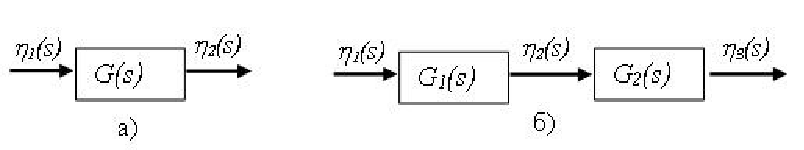
\includegraphics[width=10cm]{figures/fig_35_1.pdf}
	\caption{Структурные схемы систем со входом и выходом.}
\end{figure}

Пусть теперь выходной сигнал такой системы служит входным сигналом для второй системы, то есть, образована система из двух звеньев, соединенных последовательно (рис.\ref{fig.351} б).

Передаточная функция полученной системы по определению равна отношению преобразования Лапласа выходной функции к преобразованию Лапласа входного сигнала рассматриваемой системы. Выполняя вычисления находим, что 

\begin{equation}
\label{35.9}
	\frac {\eta_3 (s)} {\eta_1(s)}=\frac {\eta_2 (s)} {\eta_1(s)} \frac {\eta_3 (s)} {\eta_2(s)}=G_1(s) G_2(s).
\end{equation}

Итак, передаточная функция системы, состоящей из двух последовательно соединенных звеньев, равна произведению передаточных функций этих звеньев. Аналогичный результат справедлив и для систем, состоящих из любого числа последовательно соединенных звеньев. 

Теперь мы можем приступить к рассмотрению систем с обратной связью. Понятно, что системы управления, в которых используется обратная связь, должны состоять по крайней мере из двух звеньев; одно из них --- это объект управления, а другое --- управляющее устройство, или регулятор.

Объект управления --- это система, которую нужно поддерживать в определенном режиме работы; в одних случаях требуется, чтобы, несмотря на флуктуации условий сред, у нее сохранился определенный рабочий режим (система регулирования), в других --- система должна следовать изменениям того или иного параметра, характеризующего внешнюю среду (следящая система). Эти цели достигаются за счет того, что сигнал на входе объекта управления изменяется на определенную величину, зависящую от того, насколько состояние объекта управления в данный момент времени $t$ отклоняется от требуемого состояния.

Следовательно, входной сигнал объекта управления должен вырабатываться некоторой другой системой --- регулятором, который определяет, насколько состояние объекта управления отклоняется от требуемого, и затем формирует для него нужный входной сигнал, под влиянием которого это отклонение минимизируется. Для работы регулятора необходимо, чтобы он получал входные сигналы как от внешней среды, так и от самого объекта управления (это и есть то, что принято называть обратной связью). Типичная структурная схема системы с обратной связью изображена на Рис.\ref{fig.352}, где приведены общепринятые названия различных звеньев и блоков.

\begin{figure}[ht] \center
\label{fig.352}
 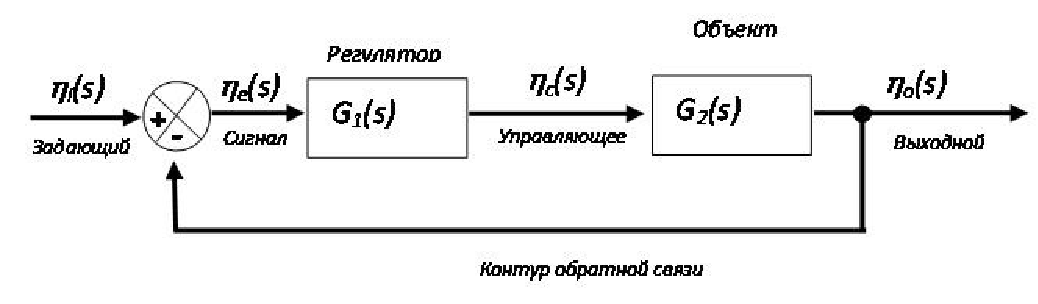
\includegraphics[width=10cm]{figures/fig_35_2.pdf}
 \caption{Типичная структурная схема системы с обратной связью.}
\end{figure}

Из передаточных функций $G_1(s)$ и $G_2(s)$, относящихся соответственно к управляющему устройству и к объекту управления, можно получить ряд других передаточных функций, характеризующих поведение всей системы с обратной связью в целом и ее отдельных частей. Во-первых, используя формулу (\ref{35.9}) находим, что

\begin{equation}
\label{35.10}
	\frac {\eta_0 (s)} {\eta_e(s)}=G_1(s) G_2(s).
\end{equation}

Выражение (\ref{35.10}) называется передаточной функцией разомкнутой системы, так как здесь не учитывается контур обратной связи. Из него можно получить две другие передаточные функции.

Вычисляя отношение $\eta_0 (s)/\eta_i(s)$, то есть передаточную функцию замкнутой системы, из (\ref{35.10}) находим
\begin{equation}
	\frac {\eta_0 (s)} {\eta_i(s)}=G_1(s) G_2(s)\frac {\eta_e (s)} {\eta_i (s)}.
\end{equation}

Но по определению $\eta_e (s)=\eta_i (s)-\eta_0 (s)$ , и поэтому 
\begin{equation}
\frac {\eta_0 (s)} {\eta_i(s)}=G_1(s) G_2(s) \left[ 1- \frac {\eta_0 (s)} {\eta_i (s)} \right].
\end{equation}

Еще раз используя (\ref{35.10}), получаем 

\begin{equation}
\label{35.11}
	\frac {\eta_0 (s)} {\eta_i(s)}=\frac {G_1(s) G_2(s)} {1+G_1(s) G_2(s)}.
\end{equation}

Наконец, принимая во внимание (\ref{35.11}), вычисляем передаточную функцию для сигнала ошибки:

\begin{equation}
\label{35.12}
	\frac {\eta_e (s)} {\eta_i(s)}=\frac {\eta_i(s)-\eta_0 (s)} {\eta_i(s)}=1-\frac{\eta_0 (s)}{\eta_i(s)}=\frac 1 {1+G_1(s) G_2(s)}.
\end{equation}

Система, изображенная на рис.\ref{fig.352}. представляет собой классическую следящую систему. Вполне очевидно, что выходной сигнал такой системы воспроизводит задающий сигнал, а свойства передаточных функций (\ref{35.10}-\ref{35.12}) позволяют оценить насколько хорошо система выполняет свое назначение.

На Рис. \ref{fig.353} показана структурная схема классической системы регулирования.

\begin{figure}[ht] \center
\label{fig.353}
	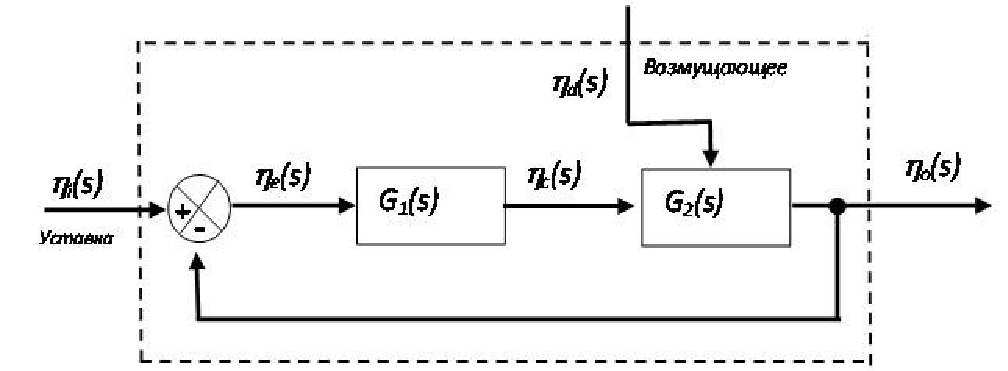
\includegraphics[width=10cm]{figures/fig_35_3.pdf}
	\caption{Структурная схема классической системы регулирования.}
\end{figure}

При работе этой системы задающий сигнал является постоянным и соответствует заданному значению регулируемой величины (это так называемая установка, например, заданное значение температуры в термостате); в этом случае приходится рассматривать еще один дополнительный входной сигнал, преобразование Лапласа которого обозначено на схеме через $\eta_d(s)$. Этот сигнал характеризует влияние флуктуаций параметров внешней среды. Как и предыдущем случае, передаточные функции, характеризующие работу системы регулирования, могут быть выписаны без труда, причем для удобства можно положить $\eta_i(s)=0$ (так что при этом $\eta_e(s)=-\eta_o(s)$):

\begin{equation}
\label{35.13}
	\frac {\eta_0 (s)} {\eta_d(s)}=G_2(s).
\end{equation}

\begin{equation}
\label{35.14}
	\frac {\eta_0 (s)} {\eta_d(s)}=\frac {G_2(s)} {1+G_1(s)G_2(s)}.
\end{equation}

\begin{equation}
\label{35.15}
	\frac {\eta_e (s)} {\eta_d(s)}=-\frac {G_2(s)} {1+G_1(s)G_2(s)}.
\end{equation}

Из формулы (\ref {35.14}) видно, что если $G1(s)G2(s)>>1$ (а это для большинства систем управления так и есть), то влияние возмущающего воздействия на величину выходного параметра уже не зависит от свойств объекта управления, а полностью определяется параметрами регулятора: 

$$ \frac {\eta_0 (s)} {\eta_d(s)} = \frac 1 {G_1(s)}$$

Причем степень влияния возмущающего воздействия на выход системы, который требуется удерживать постоянным тем меньше, чем больше передаточная функция регулятора. 

Здесь были изложены элементарные принципы классического инженерного подхода к анализу общих систем управления. Такого же рода методы исследования можно использовать при изучении механизмов управления в живых организмах. В определенных границах, присущих этому методу (его применимость ограничена тем, что он может быть использован лишь для линейных систем), такой подход к изучению физиологических систем оказался весьма плодотворным. Для биолога основной интерес представляют те специфические механизмы, которые лежат в основе изучаемой им физиологической функции, а не весь класс эквивалентных механизмов в целом. И если биолог собирается применить какую-то общую теорию, скажем, как теория систем управления, для общего исследования биологических систем, в его распоряжении должны быть определенные методы для выбора соответствующих специфических механизмов из того класса механизмов, к которому относится применяемая теория. А для этого необходим некоторый общий принцип, или критерий, лежащий вне этой теории.

Одним из таких принципов может стать принцип оптимальной конструкции, позволяющий выработать такой критерий при решении задач управления и регулирования. Главная роль принципа оптимальности в теоретической биологии заключается именно в том, что он позволяет переходить от самого общего и абстрактного рассмотрения биологических функций к одному или нескольким механизмам частного характера, которые реализуют эти функции оптимальным образом в реальных биологических системах.


\subsection{Принципы соорганизации процессов в клетке}


\begin{enumerate}
\item Специфичность катализаторов, что дает независимость процессов. (Метаболоны! --- локализации, комплексы. P-гранулы)
\item Иерархическая организация управления процессами (блоки).

Один фермент управляет большим блоком процесса. Пример из армии. Сложная система может управляться только иерархически, не могут солдаты оравой проводить военные операции. Есть у ферментов начальники.

\item Принцип относительной независимости структурных блоков в иерархии. Пояснение: необходимо, чтобы управление было завязано на содержательные сигналы. Если блок начинает реагировать еще на чужой сигнал --- это плохо, должна быть развязка. Избыток АТФ, чтобы его потребление не влияло на другие потребляющие системы. Пример: плато нагрузочной характристики, т.е. АТФаза потребляет АТФ, но концентрация АТФ к клетке не падает.

\item Режим идеального перемешивания (однородность управляемой структуры) --- особенно важно при описании реакторов. 15\% энергии клетки уходит на перемещение везикул по-кругу по цитоскелету.

\item Согласование работы ферментов, работающих в необратимых процессах (аллостерические ферменты) --- пример с фосфофруктокиназой. В процессе гликолиза она работает только в сторону расщепления глюкозы. При глюконеогенезе работает другой фермент --- бифосфатаза. В противном случае синтез глюкозы {\it de novo} был бы невозможен.
\end{enumerate}


3) Принцип независимости работы блоков. 
4) Перетаскивание вакуолей и другого для перемешивания (большой вопрос?). Водоросль может быть длинной. Однородность управляемой структуры.




\subsection{Механизмы координации внутриорганизменных химических и физиологических процессов}

Пример регуляции зрачка. Эти методы применили для системы регуляции зрачка.

Выяснилось, что обратная связь по величине не очень большая.

Когда пучок сконцентрирован в узко месте на краю, то зрачок начинает дрожать. И частота зависит от состояния мозга. Возможно это использовать для диагностики.







\newpage
%%%%%%%%%%%%%%%%%%%%%%%%%%%%%%%%%%%%%%%%%%%%%%%%%%%%%%%%%%%%%%%%%%%%%%%%%%%%%%%%%%%%%%%%
\section{Моделирование полиферментных клеточных систем}
{\it Модель энергетического метаболизма клетки. Понятие о первичной, вторичной и третичной структурах метаболизма. Режимы работы системы энергетического метаболизма.}\\
% Глава третья из Иваницкий Г.Р., Кринский В.И., Сельков Е.Е. Математическая биофизика клетки. Москва: Наука, 1978. P. 308.

% Приходится с кровью выдирать блоки модели из системы.

\subsection{Модель энергетического метаболизма клетки}



Полиферментная система --- термин для обозначения совокупности взаимосвязанных реакций, выполняющих некоторую биохимическую функцию \cite{Ivanickij1978}. Важным для экспериментального и теоретического анализа свойством полиферментных систем является их относительная автономность. Это прежде всего относится к энергетическому метаболизму. Существенная автономность позволяет проводить моделирование полиферментных систем по отдельности, без связей с остальным клеточным метаболизмом. Конечно, такое изолированное рассмотрение полиферментных систем имеет смысл только до тех пор, пока не возникает необходимость исследования их взаимодействий друг с другом. 

\subsection{Понятие о первичной, вторичной и третичной структурах метаболизма}

Тезисно (на вводной лекции):

\textbf{Первичная структура.} Если компоненты налить вокруг гейзера, то будут идти метаболические реакции.

\textbf{Вторичная.} При обособлении, появляется возможность взаимодействия через кофакторы. Появляется обратная связь, конечная стадия реакция знает что в начале. Появляется принцип 4. Клетке лучше, чтобы <<плато нагрузочной характеристики>> было пошире и поположе.

\textbf{Третичная.} Дополненная аллостерическими обратными связями в ходе эволюции.

Циркадные ритмы. Изменение характеристик и изменению суток. 23 часа для человека.


{\bf Уровни функциональной организации полиферментных систем}

Превращение исходных субстратов клеточного метаболизма, поступающих из окружающей клетку среды, в конечные продукты, выбрасываемые в среду, и в резервные вещества осуществляется через сеть взаимосвязанных ферментативных реакций, имеющих очень сложную функциональную организацию. Это функциональная организация представляет собой определенный порядок взаимодействия веществ в клетки друг с другом на основе стерического (структурного) соответствия микро- и макромолекул. Такое стерическое соответствие лежит в основе специфичности изо- и аллостерических регуляторных взаимодействий и, наконец, специфичности взаимодействий белков и нуклеиновых кислот между собой и друг с другом. Эта организация, названная организацией на основе специфичности, может существовать даже в условиях идеального перемешивания внутриклеточной среды. 

{\bf Первичная структура} клеточного метаболизма представляет собой скелет метаболизма, образованный взаимодействиями между смежными реакциями через общие промежуточные вещества. Изображение первичной структуры гликолиза показано на \ref{fig.361}. Есть основания считать, что метаболические пути (т.е. первичная структура) возникли в эволюции раньше, чем ферменты, катализирующие эти пути.

\begin{figure}[h!] \center
	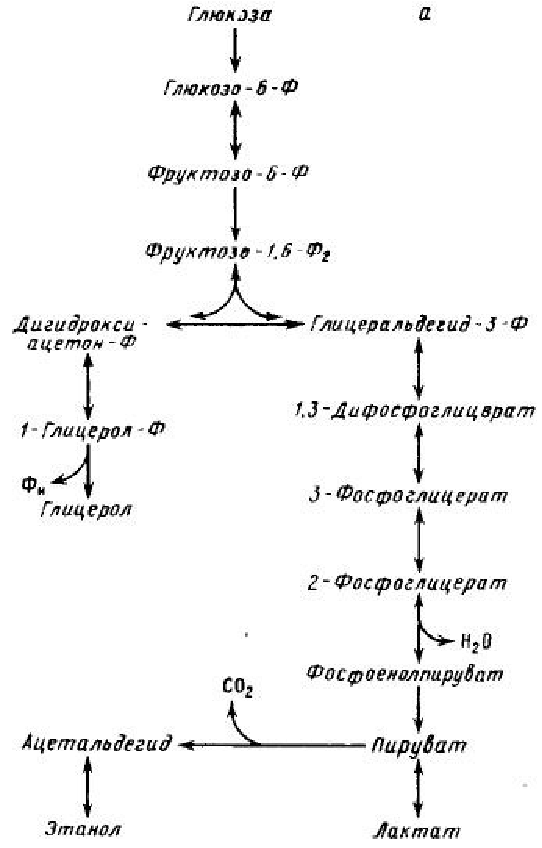
\includegraphics[width=7cm]{figures/fig_36_1.pdf}
	\caption{Схема первичной структуры гликолиза \cite{Ivanickij1978}}
 	\label{fig.361}
\end{figure}

{\bf Вторичная структура}, или стехиометрическая, клеточного метаболизма образуется из первичной структуры и взаимодействий между реакциями через общие кофакторы. Вторичная структура --- это совокупность всех стехиометрических взаимодействий между реакциями. На \ref{fig.362} показана вторичная структура гликолитической системы. Как видно из рисунка, взаимодействия четырех фосфотрансферазных реакций вызывают спирализацию первичной структуры (выделена толстой линией). 

Множество ферментативных реакций, связанных общим кофактором, образуют ядро реакции. На \ref{fig.362} показаны два ядра, образованных четырьмя фосфотрансферазными и тремя дегидрогеназными реакциями. Благодаря таким ядрам осуществляется очень тесная связь между отдельными частями первичной структуры.

\begin{figure}[h!] \center
	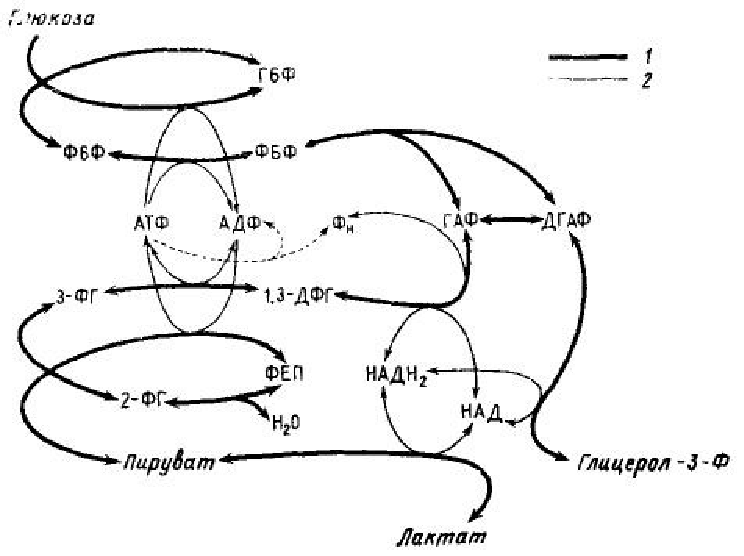
\includegraphics[width=8cm]{figures/fig_36_2.pdf}
	\caption{Схема вторичной структуры гликолиза \cite{Ivanickij1978}}
	\label{fig.362}
\end{figure}

{\bf Третичная структура} клеточного метаболизма представляет собой совокупность всех стехиометрических и нестехиометрических взаимодействий, контролирующих активности ферментов. К нестехиометрическим взаимодействиям относятся любые изо- и аллостерические взаимодействия между ферментами и модификаторами их каталитической активности. На \ref{fig.363} в качестве примера показана третичная структура гликолитической системы. Регуляторные связи третичной структуры, по-видимому, возникли в ходе эволюции и улучшили свойства вторичной структуры. Если это так, то в наших руках оказывается очень простой метод математического анализа полиферментных систем. На основании анализа вторичной структуры можно теоретически предсказать, какие нестехиометрические регуляторные взаимодействия следует внести во вторичную структуру, чтобы улучшить ее свойства. Если предсказанные регуляторные связи действительно существуют, то это указывает на то, что улучшаемое ими свойство полиферментной системы, обнаруженное на уровне вторичной структуры, играет важную роль в функциональной организации клетки. 

\begin{figure}[ht!] \center
 	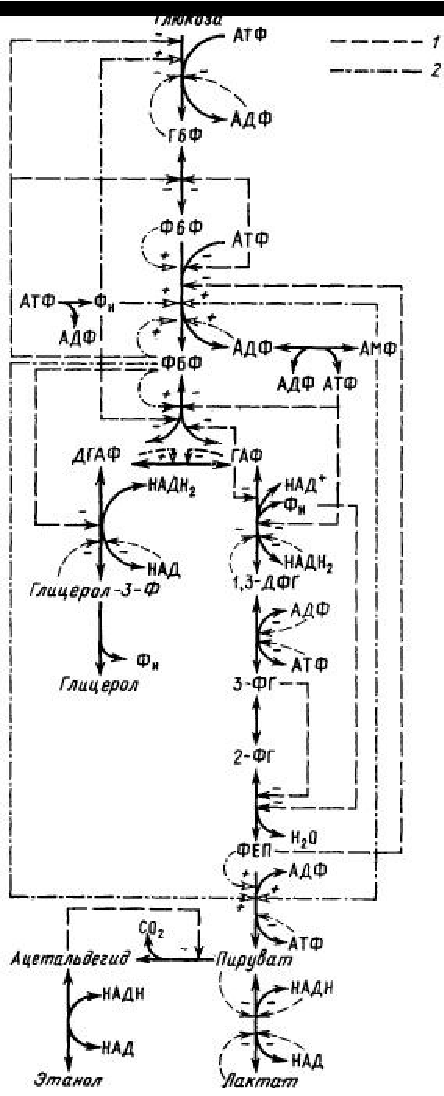
\includegraphics[width=5.7cm]{figures/fig_36_3.pdf}
	\caption{Схема третичной структуры гликолиза \cite{Ivanickij1978}}
	\label{fig.363}
\end{figure}


{\bf Простая модель стехиометрической структуры энергетического метаболизма}

Гликолиз и окислительное фосфорилирование имеют автокаталитическую, точнее рефлексивно-каталитическую, стехиометрическую структуру: их продукт АТФ участвует в <<активации>> субстратов окисления, используемых для фосфорилирования АДФ. В гликолизе активация заключается в фосфорилировании гексоз, в окислительном фосфорилировании --- в ацилировании кофермента А или карбоксилировании пирувата. Энергозависимый транспорт субстратов окисления через клеточную или митохондриальную мембраны также можно рассматривать как один из этапов активации. 

Совокупность реакции, участвующих в энергетическом метаболизме, можно упрощенно представить кинетической моделью, показанной на \ref{fig.364}.

\begin{figure}[ht] \center
	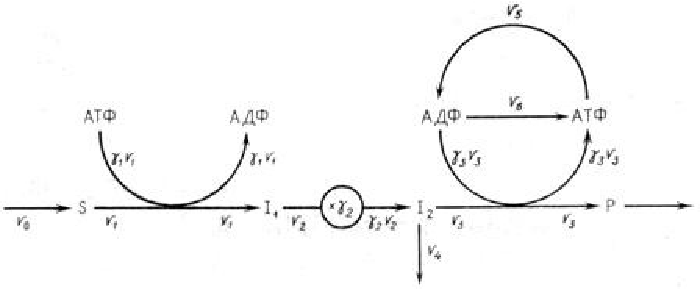
\includegraphics[width=6cm]{figures/fig_36_4.pdf}
	\caption{Упрощенная кинетическая модель энергетического метаболизма.}
	\label{fig.364}
\end{figure}

В этой модели $S$ --- субстрат, $I_1$ и $I_2$ --- интермедиаты, $P$ --- продукт окисления. При анализе схемы принято, что неорганический фосфат и окисляющий $I_2$ кофакторы имеются в избытке. Принимается также, что скорости реакций Рис.\ref{fig.364} могут быть описаны простыми выражениями (\ref{rSpeeds}).

\begin{equation}
\label{rSpeeds}
\begin{aligned}
v_0 &= v_{0m} - k_0[S],\\
v_1 &= k_1[ATP][S]/(K_1+[S]),\\
v_2 &= k_2[I_1],\\
v_3 &= k_3[I_2][ADP],\\
v_4 &= k_4[I_2],\\
v_5 &= V_5[ATP]/(K_5+[ATP]),\\
v_6 &= k_6[ADP]
\end{aligned}
\end{equation}
и что существует линейный интеграл $[ATP]+[ADP]=A_0=const$.

После перехода к безразмерным переменным, выделения малых параметров и стандартных упрощений с использованием теоремы Тихонова исходная система сводится к системе двух дифференциальных уравнений, соответствующих схеме реакции, изображенной на Рис. \ref{fig.365}.

\begin{figure}[ht] \center
	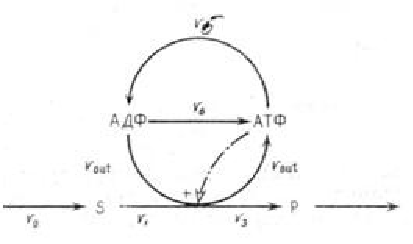
\includegraphics[width=6cm]{figures/fig_36_5.pdf}
	\caption{Редуцированная кинетическая модель энергетического метаболизма.}
	\label{fig.365}
\end{figure}

На схеме штрих-пунктирной стрелкой обозначено автокаталитическое участие АТФ в собственном синтезе. Подобное свертывание сложной полиферментной системы к одной эквивалентной реакции открывает большие возможности для упрощения анализа клеточного метаболизма.

Важнейшей количественной характеристикой любого энергетического метаболизма является его нагрузочная характеристика. Под нагрузочной характеристикой подразумевается зависимость стационарной концентрации АТФ от активности обобщенной АТФазы (нагрузки), представляющей суммарную активность всех биохимических процессов, потребляющих АТФ. Семейство нагрузочных характеристик, построенных с помощью полученной модели энергетического метаболизма приведено на Рис. \ref{fig.366}. Как видно из Рис. \ref{fig.365} при малой активности утечки нагрузочная характеристика обладает важной особенностью: с изменением нагрузки в широком диапазоне стационарная концентрация АТФ меняется очень слабо. Таким образом стехиометрическая структура энергетического метаболизма (\ref{fig.364}) способна без участия каких-либо аллостерических регуляторных связей с высокой точностью поддерживать стабильную концентрацию АТФ в широком диапазоне изменений нагрузки. 

{\it Плато очень нужно, чтобы обособить подсистемы. Чтобы потребление АТФ одной системой не влияло на другие системы.}

\begin{figure}[ht] \center
	\label{fig.366}
	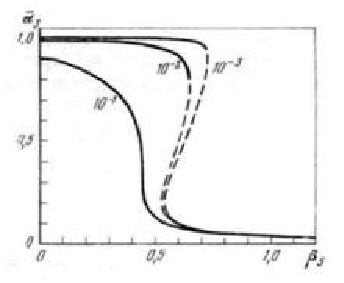
\includegraphics[width=4cm]{figures/fig_36_6.pdf}
	\caption{Семейство стационарных нагрузочных характеристик энергетического метаболизма при различных активностях утечки $(k_4)$.}
\end{figure}

Таким образом, из анализа стехиометрической структуры энергетического метаболизма и с помощью различных обобщений этой модели следует, что плато и гистерезис нагрузочной характеристики являются фундаментальными свойствами любого энергетического метаболизма, имеющего автокаталитическую природу.

На основании анализа стехиометрической структуры энергетического метаболизма можно высказать предположение, что плато и гистерезис нагрузочной характеристики должны быть объектами тонкой регуляции, осуществляемой на уровне третичной структуры. Это предположение основано на том, что оба свойства имеют очевидную ценность для клеточного обмена. Действительно, наличие четко выраженного плато означает точную стабилизацию уровня АТФ, необходимую {\bf для независимой и поэтому стабильной работы систем}, потребляющих АТФ. Что касается гистерезиса нагрузочной характеристики, то он может быть основой для временной организации не только энергетического метаболизма, но и всего клеточного обмена.


\newpage
\renewcommand{\bibname}{Список литературы}
\addcontentsline{toc}{chapter}{Список литературы}
\bibliographystyle{ugost2008}
\bibliography{library}  % собирать командой bibtexu

% эти книги пока не добавлены в bib файл
%\begin{thebibliography}{00}

%\bibitem{Meshalkin2000} Мешалкин Ю.П. Основы биофизики: Учеб. пособие.--- Новосибирск: Изд-во Новосибирск. гос. техн. ун-та, 2000.--- С. 3.
%
%\bibitem{Beresin1979}
%Березин И.В., Варфоломеев С.Д. Биокинетика.--- М.: <<Наука>>, 1979.--- 312 c.
%
%\bibitem{Varfolomeev2005}
%Варфоломеев С.Д. Химическая энзимология.--- М.: Издательский центр <<Академия>>, 2005.--- 480 с.

%\bibitem{USSRdict} См.: Советский энциклопедический словарь / Глав. ред. А.М. Прохоров.--- М.: Сов. энциклопедия, 1987.--- С. 142.
%
%\bibitem{Popova2000} 
%С.С. Попова, Некоторые аспекты междисциплинарного взаимодействия физики и биологии в научных исследованиях // Филосифия науки, т. 17, №2, --- 2003.
%
%\end{thebibliography}

\end{document}